\documentclass[hidelinks, french]{article} %MAJ 1
\usepackage[a4paper, total={6.25in, 9.5in}]{geometry}
% get fontsized kido
\usepackage{fontsize}
  \changefontsize[15]{12}
\usepackage{amsmath}\usepackage{amssymb}\usepackage{mathcomp}

\usepackage{xcolor}\usepackage{mathrsfs}\usepackage{euscript}\usepackage{wasysym}[mathcal]\usepackage{stmaryrd}\usepackage{rsfso}
% pour les belles fonts
\usepackage{amsfonts}\usepackage{bbm} \DeclareMathAlphabet{\mathpzc}{OT1}{pzc}{m}{it}
% pour pouvoir utiliser les caractères accentués
\usepackage[utf8]{inputenc}
\usepackage[T1]{fontenc}
% pour des enumerate + fancy
\usepackage{enumitem}
% pour les refs
\usepackage{cite}
% pour les beaux tableaux
\usepackage{multirow}
% pour gérer les figures
\usepackage{graphicx}
\usepackage{wrapfig}
% pour des matrices infernales
\usepackage{easybmat}
% pour rendre lien cliquable
\usepackage[colorlinks=false, %true,
            linkcolor=blue,
            citecolor=black,
            urlcolor=red]{hyperref}
% pour dessins et les diagrams
\usepackage{tikz}\usepackage{tikz-cd}
% pour les maxis plots
\usepackage{pgfplots}\pgfplotsset{compat=newest}
\usepgfplotslibrary{statistics}\usepgfplotslibrary{fillbetween}
%\usetikzlibrary{external}\tikzexternalize % speed up compilation
\usepackage{nicefrac}
% pour les maxis graphs
\usepackage{scalerel}\usepackage{pict2e}\usepackage{tkz-euclide}
\usetikzlibrary{calc}\usetikzlibrary{patterns,arrows.meta} \usetikzlibrary{shadows}\usetikzlibrary{external}
% pour la prog
\usepackage{algpseudocode}
\usepackage{fancyvrb}\usepackage{listings}
% pour la prog -test-
\usepackage{pythontex}



%%%%    RACCOURCIS    %%%%
 
\newcommand{\N}{\mathbb{N}}
\newcommand{\Z}{\mathbb{Z}}   
\newcommand{\Q}{\mathbb{Q}}
\newcommand{\R}{\mathbb{R}}
\newcommand{\C}{\mathbb{C}}
\newcommand{\K}{\mathbb{K}}
\renewcommand{\k}{\Bbbk}
\newcommand{\U}{\mathbb{U}}
\renewcommand{\u}{\text{U}}
\newcommand{\A}{\mathbb{A}}
\newcommand{\T}{\mathscr{T}}
\newcommand{\I}{\mathbb{I}}
\newcommand{\F}{\mathcal{F}}
\renewcommand{\S}{\mathfrak{S}}
\newcommand{\matk}{\mathpzc{M}_n(\mathbb{K})}
\newcommand{\matr}{\mathpzc{M}_n(\mathbb{R})}
\newcommand{\lr}{\longrightarrow}
\newcommand{\Lr}{\Longrightarrow}
\renewcommand{\ll}{\longleftarrow}
\newcommand{\Ll}{\Longleftarrow}
\newcommand{\llr}{\longleftrightarrow}
\newcommand{\Llr}{\Longleftrightarrow}
\newcommand{\para}{\sslash}
\newcommand{\Arccos}{\text{Arccos}} 
\newcommand{\Arcsin}{\text{Arcsin}} 
\newcommand{\Arctan}{\text{Arctan}} 
\newcommand{\Argch}{\text{Argch}}       
\newcommand{\Argsh}{\text{Argsh}}
\newcommand{\pgcd}{\text{pgcd}}
\newcommand{\PGCD}{\text{PGCD}}
\newcommand{\ppmc}{\text{ppcm}}
\newcommand{\sign}{\text{sign}}
\renewcommand{\Vec}{\text{Vec}}
\newcommand{\Aff}{\text{Aff}}
\newcommand{\sgn}{\text{sgn}}
\newcommand{\Deg}{\text{Deg}}
\newcommand{\ord}{\text{ord}}
\renewcommand{\det}{\text{det}}
\newcommand{\Ker}{\text{Ker}}
\newcommand{\Ann}{\text{Ann}}
\newcommand{\codim}{\text{codim}}
\newcommand{\tr}{\text{tr}}
\newcommand{\rg}{\text{rg}}
\newcommand{\Co}{\text{com}}
\newcommand{\Sp}{\text{Sp}} 
\newcommand{\GL}{\text{GL}}
\newcommand{\GA}{\text{GA}}
\newcommand{\SL}{\text{SL}}
\newcommand{\SO}{\text{SO}}
\newcommand{\HT}{\text{HT}}
\newcommand{\im}{\text{Im}}
\renewcommand{\div}{\text{div}}
\newcommand{\rot}{\text{rot}}
\renewcommand{\O}{\varnothing}
\renewcommand{\epsilon}{\varepsilon}
\renewcommand{\subsetneq}{\varsubsetneq}
\renewcommand{\leq}{\leqslant}
\renewcommand{\geq}{\geqslant}
\renewcommand{\AC}{\sim}
\renewcommand{\limsup}{\varlimsup}
\renewcommand{\liminf}{\varliminf}
\renewcommand{\stop}{\text{\;{\scriptsize$\top$}\;}}
\newcommand{\sbot}{\text{\;{\scriptsize$\bot$}\;}}
% Du grec
\newcommand{\cf}{\textit{cf. }}
\newcommand{\apriori}{\textit{a priori}}
\newcommand{\afortiori}{\textit{a fortiori}}
\newcommand{\etal}{\textit{et al. }}
\newcommand{\ei}{\textit{e.i. }}
\newcommand{\eg}{\textit{e.g. }}
% Avec Paramètre
\newcommand{\argmin}[1]{\underset{#1}{\text{argmin}}}
\newcommand{\argmax}[1]{\underset{#1}{\text{argmax}}}
\newcommand{\Top}[1]{\underset{#1}{\ \text{\huge{$\top$}}}\ }
\newcommand{\Topp}[2]{\ \underset{#1}{\overset{#2}{\text{\huge{$\top$}}}}\ }
\newcommand{\Bot}[1]{\underset{#1}{\ \text{\huge{$\bot$}}}\ }
\newcommand{\Bott}[2]{\ \underset{#1}{\overset{#2}{\text{\huge{$\bot$}}}}\ }
% Spécial TOPO
\renewcommand{\bf}[1]{\boldsymbol{#1}}
\newcommand{\V}{\mathpzc{V}}
\newcommand{\BV}{\mathpzc{BV}}
\newcommand{\Fr}{\text{Fr}}
\newcommand{\Lim}{\text{Lim}}
\newcommand{\Limf}[2]{\underset{#1}{\text{Lim}}(#2)}
\newcommand{\ring}[1]{\overset{\circ}{#1}}
\newcommand{\Ring}[1]{\overset{\circ}{\widehat{#1}}}




%%%%    SET UP    %%%%




% set up bas/haut de page

\usepackage{fancyhdr}
\pagestyle{fancy}                       
\fancyhf{}
\renewcommand{\headrulewidth}{0pt}
\cfoot{\thepage}



% set up des sections (FROM SCRATCH !!!)

\usepackage[loadonly, toctitles, clearempty]{titlesec}
            
    % génère les sections
\titleclass{\part}[-2]{top}
\titleclass{\section}{straight}[\part]
\titleclass{\subsection}{straight}[\section]
\titleclass{\subsubsection}{straight}[\subsection]

    % génère les numérotations avec format
%\newcounter{part}
\renewcommand{\thepart}{\Roman{part}}
%\newcounter{section}
\renewcommand{\thesection}{\Roman{section}.}
%\newcounter{subsection}
\renewcommand{\thesubsection}{\arabic{section}.\arabic{subsection}.}
%\newcounter{subsubsection}
\renewcommand{\thesubsubsection}{\arabic{section}.\arabic{subsection}.\arabic{subsubsection}.}

    % formatage

\titleformat{\part}[display]{\bfseries\scshape\Large}{\centering \rule{3.5cm}{0.4pt}\qquad Chapitre\quad \thechapter \qquad \rule{3.5cm}{0.4pt}}{15pt}{\centering}
\titlespacing{\chapter}{0pt}{50pt}{80pt}
\newcommand{\chapterbreak}{\clearpage}


\titleformat{\section}{\bfseries\Large}{\thesection}{15pt}{}
\titlespacing{\section}{10pt}{15pt}{10pt}

\titleformat{\subsection}{\bfseries\large}{\thesubsection}{15pt}{}
\titlespacing{\subsection}{20pt}{15pt}{10pt}

\titleformat{\subsubsection}{\bfseries}{\thesubsubsection}{15pt}{}
\titlespacing{\subsubsection}{30pt}{15pt}{10pt}


% le TOC en légende

\usepackage{titletoc}
%\contentsmargin{2em}

\titlecontents{part}[]{\rule{\textwidth}{0.5}\\* \bfseries\large\scshape Partie }{\contentslabel{15em}}{}{\hfill\contentspage}[\rule{\textwidth}{0.5}\quad]

\titlecontents{section}[2em]{\addvspace{0.5em}\bfseries}{\contentslabel{1.75em}}{\hspace*{-1.75em}}{\titlerule*[0.75pc]{.}\contentspage}[\addvspace{0.25em}]

\titlecontents{subsection}[3.5em]{\normalfont}{\contentslabel{2em}}{\hspace*{-2em}}{\titlerule*[0.75pc]{.}\contentspage}

\titlecontents{subsubsection}[5.75em]{\normalfont}{\contentslabel{2.25em}}{\hspace*{-2em}}{\titlerule*[0.75pc]{.}\contentspage}

% set up annexes
\newenvironment{annexe}{%
    \newpage
    % changement title sec
    \titleformat{\section}[display]{\bfseries\scshape\Large}{\centering}{15pt}{\centering}
    \titlespacing{\section}{0pt}{30pt}{40pt}
    
    \titleformat{\subsection}{\bfseries\large}{Annexe \thesubsection\quad ---\quad}{0pt}{}
    
    \titleformat{\subsubsection}{\bfseries}{\thesubsubsection}{15pt}{}
    
    % changement title toc
    \titlecontents{section}[0.25em]{\addvspace{0.5em}\bfseries}{}{\hspace*{-1.5em}}{\titlerule*[0.75pc]{.}\contentspage}
    
    \titlecontents{subsection}[1.5em]{\normalfont Annexe\hspace*{2.5em}}{\contentslabel{2em}}{\hspace*{-2em}}{\titlerule*[0.75pc]{.}\contentspage}
    
    \titlecontents{subsubsection}[5.75em]{\normalfont}{\contentslabel{2.25em}}{\hspace*{-2em}}{\titlerule*[0.75pc]{.}\contentspage}
    
    % changment de la numéritations
    \renewcommand{\thesubsection}{\Alph{subsection}}
    \renewcommand{\thesubsubsection}{\Alph{subsection}.\arabic{subsubsection}.}
    
    % mise à zéro des compters
    %\setcounter{section}{0}
    }{}



% set up nom des tables et références
\renewcommand{\contentsname}{}%\begin{center}\textsc{Tables des Matrières}\end{center}}
\renewcommand{\listfigurename}{\begin{center}\textsc{Table des Figures}\end{center}}
\renewcommand{\lstlistlistingname}{\begin{center}\textsc{Table des Codes}\end{center}}
\renewcommand{\refname}{\begin{center}\textsc{Références}\end{center}}



% set up des captions figures (extrêmement BG) :
\usepackage{subcaption}
\usepackage{floatrow}
\captionsetup{justification=centering}
\DeclareCaptionLabelFormat{custom}{\textit{fig. #2}}
\DeclareCaptionLabelSeparator{custom}{\, ---\, }
\DeclareCaptionFormat{custom}{#1#2#3}
\DeclareCaptionFont{custom}{\itshape }
\renewcommand{\thefigure}{\arabic{figure}}
\newcommand{\figref}[1]{\textit{fig.\,\ref{#1}}}
    % espacement pour les wrapfig (casse tout pour les multirow format)
%\renewcommand{\columnsep}{1cm}

% set up ENONCES (PROP, DEF, RQ) :
\usepackage{amsthm}

\newtheoremstyle{enonce}{0pt}{25pt}{}{}{\scshape}{\quad ---\quad }{0em}{}
\newtheoremstyle{special}{0pt}{25pt}{}{}{\scshape}{\quad ---\quad }{0em}{\thmnote{#3}}
\newtheoremstyle{rq}{0pt}{25pt}{\itshape}{}{\scshape}{\quad ---\quad}{0em}{}
\newtheoremstyle{exo}{0pt}{25pt}{\color{blue}}{}{\scshape\color{blue}}{: \newline}{0em}{}
\newtheoremstyle{demo}{8pt}{0pt}{\color{mygray}}{}{\itshape\color{mygray}}{\newline\newline}{0em}{}

\theoremstyle{enonce}
\newtheorem{definition}{Définition}
\newtheorem{proposition}{Proposition}
\newtheorem{propriete}{Propriété}
\newtheorem{propricarac}[propriete]{Propriété Caractéristique}
\newtheorem{lemme}{Lemme}
\newtheorem{theoreme}{Théorème}
\newtheorem{theodef}[theoreme]{Théorème et Définition}
\newtheorem{corollaire}{\qquad Corollaire}[theoreme]
\newtheorem{assump}{Hypothèse}

\theoremstyle{special}
\newtheorem{enonce}{}

\theoremstyle{rq}
\newtheorem*{remarque}{\qquad Remarque}
\newtheorem*{rappel}{\qquad Rappel}
\newtheorem*{exemple}{\qquad Exemple}

\theoremstyle{exo}
\newtheorem{exercice}{Exercice}

\definecolor{mygray}{gray}{0.3}
\theoremstyle{demo}
\newtheorem*{demo}{\qquad\qquad\qquad\rule{3.5cm}{0.4pt}\qquad\quad Démonstration\qquad\quad \rule{3.5cm}{0.4pt}}
%\begin{center}\rule{8cm}{0.4pt}\end{center}


% set up plot
\pgfplotsset{standard/.style={width=0.4\textwidth,
    height=0.22\textwidth,
    trig format=rad,
    enlargelimits,
    enlarge x limits=0.05,
    enlarge y limits=0.05,
    every axis x label/.style={footnotesize, at={(current axis.right of origin)},anchor=north west},
    every axis y label/.style={footnotesize, at={(current axis.above origin)},anchor=south east},
    every tick label/.append style={font=\scriptsize},
    scale only axis=true}}
\pgfplotsset{compar/.style={width=0.4\textwidth,
    height=0.2\textwidth,
    trig format=rad,
    enlargelimits,
    enlarge x limits=0.05,
    enlarge y limits=0.05,
    every axis x label/.style={footnotesize, at={(current axis.right of origin)},anchor=north west},
    every axis y label/.style={footnotesize, at={(current axis.above origin)},anchor=south east},
    every tick label/.append style={font=\scriptsize},
    scale only axis=true}}
\pgfplotsset{small/.style={width=0.2\textwidth,
    height=0.08\textwidth,
    trig format=rad,
    enlargelimits,
    enlarge x limits=0.05,
    enlarge y limits=0.05,
    every axis x label/.style={footnotesize, at={(current axis.right of origin)},anchor=north west},
    every axis y label/.style={footnotesize, at={(current axis.above origin)},anchor=south east},
    every tick label/.append style={font=\scriptsize},
    scale only axis=true}}
\pgfplotsset{speAE/.style={width=0.27\textwidth,
    height=0.16\textwidth,
    trig format=rad,
    enlargelimits,
    enlarge x limits=0.05,
    enlarge y limits=0.05,
    every axis x label/.style={at={(current axis.right of origin)},anchor=north west},
    every axis y label/.style={at={(current axis.above origin)},anchor=south east},
    every tick label/.append style={font=\scriptsize},
    scale only axis=true}}
\pgfplotsset{nobox/.style={width=4.5cm,
    height=3.5cm,
    %compat=1.18,
    trig format=rad,
    enlargelimits,
    axis x line=middle,
    axis y line=middle,
    enlarge x limits=0.15,
    enlarge y limits=0.15,
    every axis x label/.style={at={(current axis.right of origin)},anchor=north west},
    every axis y label/.style={at={(current axis.above origin)},anchor=south east},
    every tick label/.append style={font=\scriptsize},
    scale only axis=true}}

    %preset prog    
\definecolor{codeblack}{rgb}{0.01,0.01,0.01}
\definecolor{codegreen}{rgb}{0,0.6,0}
\definecolor{codegray}{rgb}{0.5,0.5,0.5}
\definecolor{codepurple}{rgb}{0.58,0,0.82}
\definecolor{backcolour}{rgb}{0.98,0.98,0.95}
\definecolor{textgray}{rgb}{0.97,0.97,0.95}
\lstdefinestyle{pur}{
    backgroundcolor=\color{backcolour},   
    commentstyle=\color{codegray},
    keywordstyle=\color{orange},
    numberstyle=\tiny\color{codegray},
    stringstyle=\color{codegreen},
    basicstyle=\ttfamily\footnotesize,
    breakatwhitespace=false,         
    breaklines=true,                 
    captionpos=b,                    
    keepspaces=true,                 
    numbers=left,                    
    numbersep=5pt,                  
    showspaces=false,                
    showstringspaces=false,
    showtabs=false,                  
    tabsize=2,
    frame=single,
    rulecolor=\color{lightgray}}
\lstdefinestyle{informal}{%useless
    basicstyle=\footnotesize,
    breakatwhitespace=false,         
    breaklines=true,                 
    captionpos=b,                    
    keepspaces=true,               
    showspaces=false,                
    showstringspaces=false,
    showtabs=false,                  
    tabsize=2,
    frame=single,
    rulecolor=\color{black}}
\lstset{style=pur}
\newcommand{\pyt}[1]{{\footnotesize{\colorbox{textgray}{\color{mygray}\texttt{#1}}}}}
    



\title{\textbf{\textsc{JSP encore}\newline Rapport de Stage de M1}}
\author{}
\date{Grégoire \textsc{Doat}}
\begin{document}

\captionsetup{labelformat=custom, labelsep=custom}
\alglanguage{pseudocode}

\begin{titlepage}\centering
	{\color{white}l}

	\vspace{1cm}
	
	{\Large\textbf{\textsc{Rapport de Stage}}}
 
    \vspace{1.5cm}
    
	{\huge\scshape\textbf{Super-Résolution d'Images via}}
 
    \vspace{0.2cm}
    
    {\huge\scshape\textbf{Réseau Autoencodeur}}
    
	\vspace{1.5cm}
 
	{\large Grégoire \textsc{Doat}}\par
 
	\vspace{0.5cm}
 
	\quad{\large Sous la tutelle de M. Yann \textsc{Traonmilin}}

     %\vfill
     \vspace{0.5cm}
 
	\rule{10cm}{0.3pt}\par
 
	\vspace{0.7cm}
    {\large Mai -- Juin 2024}

    
    \vfill
    %{\Large\textbf{Résumé}}\par}
    \tableofcontents

    
    %\vspace{1cm}
	%On augmente la résolution de l'image sans apprentissage (faut voir comment) puis on utiliste un algorithme d'amélioration de la résolution. C'est pas mal parce que ça permet de réutiliser ce qui existe déjà sur l'amélioration d'image (rébruitage par exmple).

    %Clairement, ce a ses limites, l'augmentation de résolution est pas forcément la plus maligne et l'appentissage est pas possible dessus. Aussi, rien n'indique que se faisant, on ne tue pas l'information qu'un algo de néttoyage d'image utilise.


	\vspace{0.5cm}

\end{titlepage}

%\tableofcontents   \newpage

%{\color{white}l}\vfill\section*{\itshape\begin{center}Remerciements\end{center}}\emph{Lorem ipsum dolor sit amet, consectetur adipiscing elit. Sed eu tincidunt lacus. Cras scelerisque odio elementum facilisis cursus. Class aptent taciti sociosqu ad litora torquent per conubia nostra, per inceptos himenaeos. Vestibulum sollicitudin vulputate luctus. Mauris tincidunt mattis purus eu eleifend. Curabitur sodales est eu sapien fringilla volutpat. Curabitur vestibulum porta diam, ac sagittis libero commodo eu. Pellentesque elementum magna vitae eros ultrices, vel tempus orci suscipit. Praesent velit diam, bibendum eu euismod sit amet, volutpat eu erat. Suspendisse vel faucibus urna, a maximus quam. }\vfill\vfill\vfill{\color{white}l}\newpage





\phantomsection
\addcontentsline{toc}{section}{Introduction}
\section*{Introduction}
{\color{white}bllblblb}

Dans ce rapport de stage on s'intéresse au problème de super-résolution. C'est-à-dire la reconstruction d'image $\bf{x}$, disons de taille $(n,m)$, à partir d'une version sous-échantillonné $\bf{y}$ de taille $(p,q)$ et se pose ainsi\footnote{ce n'est pas nécessairement la seule façon de poser le problème cela dit} : 

Étant donnée une image $\bf{x_0}\in\R^{n\times m}$ et sa version sous-échantillonnée $\bf{y_0}\in\R^{p\times q}$ on cherche à minimiser la fonctionnelle :\begin{equation}\label{eq:F}
F :\quad \begin{aligned}\R^{n\times m}\ &\lr\qquad\quad \R \\ \bf{x}\quad\ &\longmapsto\ \frac{1}{2}{\big\|A\bf{x}-\bf{y_0}\big\|_2}^2\end{aligned}\end{equation}
\\
que l'on suppose convexe et où $A$ représente le sous-échantillonage, aussi appelée opérateur de mesure puisque l'on peut l'interpréter comme une mesure incomplètement d'une ``véritable'' image. 
\\

Par nature, l'application $A$ n'est pas injective, elle ne conserve pas toute l'information originale. Cela fait rentrer le problème de super-résolution dans la classe des problèmes inverses mal posés.
\\

Une façon de retrouver (au moins partiellement) l'injectivité de $A$ consiste à introduire une paramétrisation $\phi$ de l'espace des images $\bf{x}$ telle que $\ \phi(\theta)=\bf{x}\ $ et à chercher les bons paramètres $\theta$ plutôt que $\bf{x}$. L'intérêt étant que si le nombre de paramètre est suffisamment petit par rapport à la taille de l'espace des mesures, on peut espérer que le problème soit mieux poser en cherchant à inverser $A\phi$.
\\
Le contre coût de cette méthode est qu'elle à toute les chances  d'impacter la convexité du problème. Ce pose donc la question du comportement la fonctionnelle $\ F\circ\phi\ $ au voisinage de ses minimums. 
\\
C'est précisément ce qu'on étudier Y. Traonmilin, J.-F. Aujol et A. Leclaire  dans leur article \emph{The basins of attraction of the global minimizers of non-convex inverse problems with low-dimensional models in infinite dimension} de 2022 \cite{traonmilin_basins_2022}. Ils donnent une caractérisation d'abord générale des bassins d'attractions, c'est-à-dire l'ensemble des paramètres $\theta$ partant desquelles la descente de gradient convergerait vers un minimum globale de $\ F\circ\phi$. Puis applique leur résultat à des problèmes inverses classiques : reconstruction de matrice de bas rang, Off-the-grid sparse spike recovery, estimation de mélange de gaussiennes.
\\

Le point commun de ses trois problèmes est que l'espace des objets à reconstruire possède une paramétrisation connue et exploitable, ce qui n'est pas le cas de l'ensemble des images. En toute généralité, l'ensemble $\Sigma$ des images de taille $(n,m)$ est $\R^{n\times m}$, mais en le restreignant à un type d'images (ne serait-ce qu'en excluant les images de bruit blanc), sa structure est beaucoup moins claire et ses paramétrisations encore moins. C'est là qu'intervient le machin learning.
\\

Le but du stage est d'étudier dans quelle mesure les travaux de Traonmilin \etal s'applique au problème de super-résolution en prenant comme paramétrisation le décodeur d'un auto-encodeur entraîné sur un jeu de données (dans notre cas MNIST). 
\\
\`A côté de cela, P. Peng, S. Jalali et X. Yuan ont étudié la descente de gradient projeté pour résoudre le même problème de super-résolution en prenant comme projection un auto-encoder appris. On tentera, dans un second temps, de reproduire leur résultats pour les comparer à ceux de la descente de gradient depuis l'espace latent.
\\





\section{Cadre théorique}\label{sec:cadre theo}


\subsection{Formalisation du problème}\label{sec:forma2pb}

Soit $A$ un opérateur de mesure linéaire à valeur de $\R^{n\times m}$ dans $\R^{p\times q}$. Il se compose d'un sous-échantillonnage (projection) $S$ et d'un éventuel filtre passe-bas $C_{\bf{h}}$ pour éviter les problèmes d'aliasing. $C_{\bf{h}}$ est donc une convolution par un filtre que l'on va noter $\bf{h}$ (d'où la notation) de sorte que $A$ s'écrive :
\[\forall \bf{x}\in\R^{n\times m},\qquad A\bf{x}=S(\bf{h}*\bf{x})=SC_{\bf{h}}\bf{x}\]
Ci-dessous deux représentations de $S$ pour $(n,m)=(3, 4)$ et $(p,q)=(2, 2)$ : sur la figure \textit{\ref{fig:Simg}}, $S$ ne garde d'un pixel sur $4$ de l'image $\bf{x}$, ce qui correspond à appliquer la matrice de la figure \textit{\ref{fig:Smat}} au vecteur $\bf{x}$ aplati.

Pour affectuer la convolution avec $\bf{h}$, l'algorithme passe l'espace de fréquences, le changeant en simple produit et c'est dans cet espace que son ajuster pas les paramètres des deux filtres proposés :
\\
Le filtre gaussien à pour paramètre l'écart-type $\sigma$ de $\hat{\bf{h}}$. Pour le filtre porte, le paramètre $a$ ajuste la taille de la fenêtre $[-a,a]\times[-a,a]$ dans l'espace des fréquences. La figure \ref{fig:filtres} en donne quelque exemple, plus de détail en annexes \ref{anx:gradF}.
\\

\begin{figure}[b]
\begin{floatrow}
\ffigbox{\caption{Opérateur $S$, point de vue matriciel} \label{fig:Smat}}
{\sbox0{$\begin{array}{ c c |}
1\ 0   & 0\ 0   \\
0\ 0 &   1\ 0   \\\hline
\end{array}$}

\sbox1{$\begin{array}{| c c | c c }\hline
0\ 0  &  0\ 0  &  1\ 0   &  0\ 0   \\
0\ 0  &  0\ 0  &  0\ 0 &   1\ 0    \\%\hline
\end{array}$}



\[\left(\begin{array}{c c}
\usebox{0}  &  \makebox[\wd1]{\Large \text{$\mathbb{O}$}}  \\
\makebox[\wd0]{\huge \text{$_{\mathbb{O}}$}} &  \usebox{1}
\end{array}\right)\]
\vspace{0.4cm}


%\vphantom{\usebox{0}}}

\ffigbox{\caption{Opérateur $S$, point de vue image} \label{fig:Simg}}
{
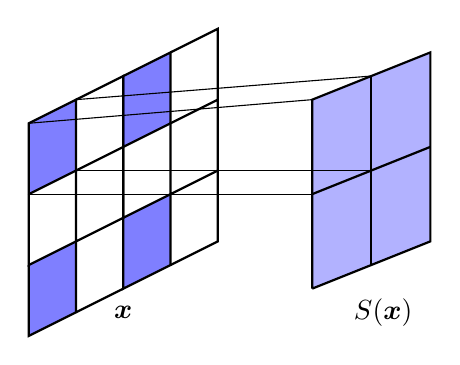
\begin{tikzpicture}[scale=0.6]
%\draw[opacity=0.5] (-4,-4) grid (4,4);

%%% grosse image

    % BLOCK (1,1)
% pixels bleu
\draw[thick, fill=blue, fill opacity=0.5] (-3,0) -- (-3,-1.5) -- (-4,-2)  -- (-4,-0.5);

% pixels blancs
\draw[thick, xshift=1cm, yshift=0.5cm] (-4,-2) -- (-3,-1.5);


    % BLOCK (2,1)
% pixels bleu
\draw[thick, fill=blue, fill opacity=0.5, xshift=2cm, yshift=1cm] (-3,0) -- (-3,-1.5) -- (-4,-2)  -- (-4,-0.5);

% pixels blancs
\draw[thick, xshift=3cm, yshift=1.5cm] (-3,0) -- (-3,-1.5) -- (-4,-2);

    % BLOCK (1,2)
% pixels bleu
\draw[thick, fill=blue, fill opacity=0.5, yshift=3cm] (-4,-2) -- (-4,-0.5) -- (-3,0) -- (-3,-1.5) -- (-4,-2);

% pixels blancs
\draw[thick, yshift=1.5cm] (-4,-0.5) -- (-4,-2) -- (-3,-1.5);
\draw[thick, xshift=1cm, yshift=3.5cm] (-4,-0.5) -- (-3,0) -- (-3,-1.5);

%pixels rouge
\draw[thick, xshift=1cm, yshift=2cm] (-4,-2) -- (-4,-0.5) -- (-3,0) -- (-3,-1.5) -- (-4,-2);

    % BLOCK (2,2)
% pixels bleu
\draw[thick, fill=blue, fill opacity=0.5, xshift=2cm, yshift=4cm] (-4,-2) -- (-4,-0.5) -- (-3,0) -- (-3,-1.5) -- (-4,-2);

% pixels blancs
\draw[thick, xshift=2cm, yshift=2.5cm] (-4,-0.5) -- (-4,-2) -- (-3,-1.5);
\draw[thick, xshift=3cm, yshift=4.5cm] (-4,-0.5) -- (-3,0) -- (-3,-1.5);

%pixels rouge
\draw[thick, xshift=3cm, yshift=3cm] (-4,-2) -- (-4,-0.5) -- (-3,0) -- (-3,-1.5) -- (-4,-2);

%%% petite image

\draw[thick, fill=blue, fill opacity=0.3, xshift=1cm] (1,-1) -- (1,3) -- (3.5,4) -- (3.5,0) -- (1,-1);
\draw[thick, xshift=2.25cm, yshift=0.5cm] (1,-1) -- (1,3);
\draw[thick, xshift=1cm, yshift=-2cm] (1,3) -- (3.5,4);

%%% lien

\draw (-4,1) -- (2,1);
\draw (-4,2.5) -- (2,3);
\draw (-3,1.5) -- (3.25,1.5);
\draw (-3,3) -- (3.25,3.5);

%%% Nom

\draw  (-2,-1.5) -- (-2,-1.5) node{$\bf{x}$};
\draw  (3.5,-1.5) -- (3.5,-1.5) node{$S(\bf{x})$};
\end{tikzpicture}}
\end{floatrow}
\end{figure}

\begin{figure}[h]\centering
    \setlength{\tabcolsep}{5pt}
\begin{tabular}{c c c c c}

\ Sans  &  $\sigma=0.5$  &  $\sigma=0.6$  &  $a=0.6$  &  $a=0.4$

\\

\rotatebox[origin=lt]{90}{{\color{white}bb}filtre}


\includegraphics[width=0.14\textwidth]{resultats/compare_filter/seed21-f-filtre=s.png}
&

\includegraphics[width=0.14\textwidth]{resultats/compare_filter/seed21-f-filtre=g_param=0.5.png}
&

\includegraphics[width=0.14\textwidth]{resultats/compare_filter/seed21-f-filtre=g_param=0.6.png}
&

\includegraphics[width=0.14\textwidth]{resultats/compare_filter/seed21-f-filtre=p_param=0.6.png}
&

\includegraphics[width=0.14\textwidth]{resultats/compare_filter/seed21-f-filtre=p_param=0.4.png}

\\

\rotatebox[origin=lb]{90}{{\color{white}b}image $\bf{x}$}


\includegraphics[width=0.14\textwidth]{resultats/compare_filter/seed21-x.png}
&

\includegraphics[width=0.14\textwidth]{resultats/compare_filter/seed21-x.png}
&

\includegraphics[width=0.14\textwidth]{resultats/compare_filter/seed21-x.png}
&

\includegraphics[width=0.14\textwidth]{resultats/compare_filter/seed21-x.png}
&

\includegraphics[width=0.14\textwidth]{resultats/compare_filter/seed21-x.png}

\\

\rotatebox[origin=lb]{90}{{\color{white}l}mesure $A\bf{x}$}


\includegraphics[width=0.14\textwidth]{resultats/compare_filter/seed21-Ax-filtre=s.png}
&

\includegraphics[width=0.14\textwidth]{resultats/compare_filter/seed21-Ax-filtre=g_param=0.5.png}
&

\includegraphics[width=0.14\textwidth]{resultats/compare_filter/seed21-Ax-filtre=g_param=0.6.png}
&

\includegraphics[width=0.14\textwidth]{resultats/compare_filter/seed21-Ax-filtre=p_param=0.6.png}
&

\includegraphics[width=0.14\textwidth]{resultats/compare_filter/seed21-Ax-filtre=p_param=0.6.png}
\end{tabular}
    \caption{Quelques exemples d'application de $A$ à un même image en fonction des filtres. }
\end{figure}

\begin{enonce}[Problématique]
On considère $\bf{x_0}\in\R^{n\times m}$ une image que l'on cherche à reconstruire et $\ \bf{y_0}:=A(\bf{x_0})\ $ sa version sous-échantillonnée. Une bonne reconstruction de $\bf{x_0}$ étant un minimiseur :
\begin{equation}\label{eq:probleme}
\bf{x^*}\in \argmin{\bf{x}\in\R^{n\times m}}\ F(\bf{x})\end{equation}\end{enonce}

Si pour le bien de l'étude $\bf{x_0}$ sera connu, il va de soit que le problème nécessite pas de le connaître \apriori.
\\
Aussi, la linéarité de $A$ assure la convexité de $F$ mais, bien évidemment, son caractère hautement non injectif (surtout pour $pq\lll nm$) fait qu'il existe tout un sous-espace affine de minimum globaux. D'où l'intérêt des deux méthodes étudiées pour ``choisir'' ce minimum.
\\

\begin{wrapfigure}{r}{0.4\textwidth}% vire le [16]
    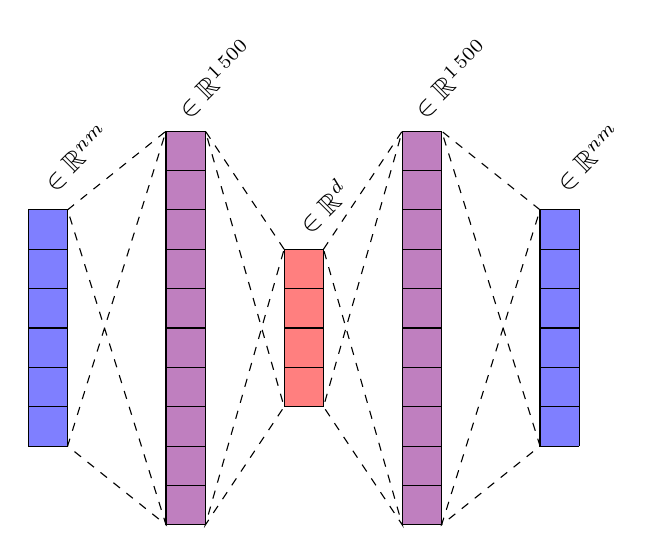
\begin{tikzpicture}[scale=0.5]
%\draw[thin, opacity=0.5] (-7.5,-6.5) grid (7.5,6.5);

%%% vecteurs

% input
\draw[fill=blue, fill opacity=0.5] (-7,-3) -- (-7,3) -- (-6,3)  -- (-6,-3) -- (-7,-3);
\draw (-7, 2) -- (-6, 2);
\draw (-7, 1) -- (-6, 1);
\draw (-7, 0) -- (-6, 0);
\draw (-7, -1) -- (-6, -1);
\draw (-7, -2) -- (-6, -2);

% hidden 1
\draw[fill=violet, fill opacity=0.5] (-3.5,-5) -- (-2.5,-5) -- (-2.5,5)  -- (-3.5,5) -- (-3.5,-5);
\draw (-3.5, 4) -- (-2.5, 4);
\draw (-3.5, 3) -- (-2.5, 3);
\draw (-3.5, 2) -- (-2.5, 2);
\draw (-3.5, 1) -- (-2.5, 1);
\draw (-3.5, 0) -- (-2.5, 0);
\draw (-3.5, -1) -- (-2.5, -1);
\draw (-3.5, -2) -- (-2.5, -2);
\draw (-3.5, -3) -- (-2.5, -3);
\draw (-3.5, -4) -- (-2.5, -4);

% latent
\draw[fill=red, fill opacity=0.5] (-0.5,-2) -- (0.5,-2) -- (0.5,2)  -- (-0.5,2) -- (-0.5,-2);
\draw (-0.5, 1) -- (0.5, 1);
\draw (-0.5, 0) -- (0.5, 0);
\draw (-0.5, -1) -- (0.5, -1);

% hidden 2
\draw[fill=violet, fill opacity=0.5] (3.5,-5) -- (2.5,-5) -- (2.5,5)  -- (3.5,5) -- (3.5,-5);
\draw (3.5, 4) -- (2.5, 4);
\draw (3.5, 3) -- (2.5, 3);
\draw (3.5, 2) -- (2.5, 2);
\draw (3.5, 1) -- (2.5, 1);
\draw (3.5, 0) -- (2.5, 0);
\draw (3.5, -1) -- (2.5, -1);
\draw (3.5, -2) -- (2.5, -2);
\draw (3.5, -3) -- (2.5, -3);
\draw (3.5, -4) -- (2.5, -4);

% output
\draw[fill=blue, fill opacity=0.5] (7,-3) -- (7,3) -- (6,3)  -- (6,-3) -- (7,-3);
\draw (7, 2) -- (6, 2);
\draw (7, 1) -- (6, 1);
\draw (7, 0) -- (6, 0);
\draw (7, -1) -- (6, -1);
\draw (7, -2) -- (6, -2);

%%% liens

\draw[dashed, thin] (-6,3) -- (-3.5,5) -- (-6,-3) -- (-3.5,-5) -- (-6,3);
\draw[dashed, thin] (-0.5,2) -- (-2.5,5) -- (-0.5,-2) -- (-2.5,-5) -- (-0.5,2);
\draw[dashed, thin] (0.5,2) -- (2.5,5) -- (0.5,-2) -- (2.5,-5) -- (0.5,2);
\draw[dashed, thin] (6,3) -- (3.5,5) -- (6,-3) -- (3.5,-5) -- (6,3);

%%% tailles

\draw (-5.75,4.25) -- (-5.75,4.25) node[]{\rotatebox[origin=lt]{45}{$\in\R^{nm}$}};
\draw (-2.25,6.25) -- (-2.25,6.25) node[]{\rotatebox[origin=lt]{45}{$\in\R^{1\,500}$}};
\draw (0.5,3) -- (0.5,3) node[]{\rotatebox[origin=lt]{45}{$\in\R^d$}};
\draw (3.75,6.25) -- (3.75,6.25) node[]{\rotatebox[origin=lt]{45}{$\in\R^{1\,500}$}};
\draw (7.25,4.25) -- (7.25,4.25) node[]{\rotatebox[origin=lt]{45}{$\in\R^{nm}$}};
\end{tikzpicture}
    \caption{Schéma des auto-encodeurs  $f$ avec $d=100,\ 200,\ 400,\ 800$}
    \label{fig:AEschem}
\end{wrapfigure}

Les auto-encodeurs utilisés pour paramétrer l'espace des images sont des réseaux MLP que l'on notera indifféremment $f$ et dont $f_E$ et $f_D$ sont les parties encodage et décodage :
\[f = f_E\circ f_D\]
Conformément à la figure \textit{\ref{fig:AEschem}}, ils se composent tous d'une couche cachées de taille $1\,500$ pour les parties encodeurs et décodeurs et la seule choses qui les différencies est la taille de leur espace latent qui variant entre $100$ et $800$. Leur entraînement s'est fait sur le jeu donnés MNIST et c'est donc uniquement sur ces images que seront présenté les résultats. Plus de détail sur les performances des auto-encodeurs en annexe \ref{anx:AE}. 
\\ 

TRANSITION ?
\\




\subsection{Cadre théorique de l'article}\label{sec:article1/2}

Comme expliqué plus tôt, tout l'objet de l'article \cite{traonmilin_basins_2022} est d'étudier dans quelle mesure il est possible de faire une descente de gradient sur une paramétrisation (non-convexe) d'un modèle plutôt que sur le modèle lui-même. 
\\
Pour cela, on note $\Sigma\subset\R^{n\times m}$ le modèle de basse-dimension et $\phi: \R^d\lr\R^{n\times m}$ une paramétrisation de ce dernier avec :
\begin{align*}\Sigma&\subset\phi\big(\R^d\big)  &  \Theta&:=\phi^{-1}(\Sigma)\end{align*}
\\
La paramétrisation $\phi$, doit vérifier certaines hypothèses de régularité pour pouvoir appliquer les résultats de l'article. Dans notre cas, $\ \phi=f_D\ $ dont les fonctions d'activations sont toutes des sigmoïdes. Elle est donc $C^{\infty}$ et pour cette raison on ne s'attardera pas outre mesure sur les questions de régularités de $\phi$.
\\

\textit{\`A noter qu'on ne suppose ni que $\ \phi(\R^d)=\Sigma\ $ ni que  $\ \Theta=\R^d$ et ce ne sera pas le cas pour nous. Aussi, le formalisme proposé par Traonmilin \etal est légèrement différent de celui donné en section précédente. Il y est considéré un espace de mesure $\mathcal{D}$ et les signaux (dans notre cas les images) sont pris dans $\mathcal{D}^*$, de sorte que la mesure par $\alpha\in\mathcal{D}$ de $x\in\mathcal{D}^*$ soit représenté par le crochet de dualité $\langle \alpha,x\rangle$. Cela à son intérêt surtout en dimension infinie, mais autrement, cette écriture est tout à fait équivalente à celle donnée en section \ref{sec:forma2pb}}
\\

\begin{wrapfigure}{r}{0.43\textwidth}
    \fbox{\begin{minipage}{15em}
\vspace{0.3cm}
\begin{algorithmic}[0]
    \State $\theta_0$ : initialisation
    \State $x$ : image à reconstruire
    \State $\tau$ : pas de descente
    \State $N$ : nombre d'itération
    \State $\hat{x}\ \longleftarrow\ f(x)$
    \State
    \For{$n\in \llbracket1,N-1\rrbracket$}
        \State $\theta_{n+1}\ \longleftarrow\ \theta_n\ - \tau \nabla g(\theta_un)$
        \State $x_{n+1}\ \longleftarrow\ f_D(\theta_{n+1})$
        \EndFor
    \State
    \Return $(x_n)_{0\leq n\leq N}$
\end{algorithmic}
\vspace{0.2cm}
\end{minipage}}
    \caption{Algorithme de descente depuis l'espace des paramètres}
    \label{fig:pcode LGD}
\end{wrapfigure}

Le problème est donc de trouver les paramètres $\theta^*$ minimisant $\ g:=A\phi\ $ sur $\Theta$, ou dans notre cas :
\[\theta^*\in\argmin{\theta\in\Theta}\ \frac{1}{2}{\big\|Af_D(\theta)-\bf{y_0}\big\|_2}^2\]
\\
Minimum que l'on cherche à les obtenir par descente de gradient. On considérera donc dans toute la suite, $(\theta_n)$ la descente de gradient à pas fixe, $\forall\theta_0\in\R^d$ :
\[\forall n\in\N^*,\qquad \theta_{n+1} = \theta_n - \tau\nabla g(\theta_n)\]
Sachant que $\phi$ est n'est pas convexe, on introduit la définition suivante :
\\ \\
\begin{definition} 
Une partie $\Lambda\subset\Theta$ de $\R^d$ sera un \emph{bassin d'attraction} de minimum globale $\theta^*\in\Lambda$ si en tout point $\theta_0\in\Lambda$, alors existe un pas de descente $\tau_0$ tel que :
\[\forall \tau\in]0,\tau_0],\qquad \lim_{n\lr+\infty}g\big(\theta_n\big)=g(\theta^*)\]
\end{definition}

Avec cette définition, $(\theta_n)$ peut tout à fait converger vers un autre minimum que $\theta^*$. Pour en tenir compte en même temps que la potentielle non-injectivité de $\phi$, ils introduisent les définitions suivantes :
\\
\begin{definition}\label{def:boule}
On note $d(\theta,\theta^*)$ la distance de $\theta$ au plus proche paramètre de même image de $\theta^*$ et $p(\theta,\theta^*)$ la projection (potentiellement multivaluée) de $\theta$ sur ce même paramètre, e.i. sur $\phi^{-1}\circ\phi(\{\theta^*\})$ :
 $\forall\theta\in\R^d$ :
\begin{align*}d(\theta,\theta^*) &:=\min_{\substack{\Tilde{\theta}\in\Theta\\ \phi(\Tilde{\theta})=\phi(\theta^*)}}\ \big\|\Tilde{\theta}-\theta\big\|_2  &  p(\theta,\theta^*)&:=\argmin{\substack{\Tilde{\theta}\in\Theta\\ \phi(\Tilde{\theta})=\phi(\theta^*)}}\ \big\|\Tilde{\theta}-\theta\big\|_2\subset\R^d\end{align*}
Avec, sont définis les bassins $\Lambda_\beta(\theta^*)$ de la forme :
\[\forall \beta\in\R^{+_*},\qquad \Lambda_\beta(\theta^*):=\big\{\theta\in\R^d\ |\ d(\theta, \theta^*)<\beta\big\}\]
\end{definition}

Contrairement aux exemples traités dans l'article, la paramétrisation par l'espace latent ne donne pas de formule vraiment exploitable pour $\phi=f_D$. En revanche, $f_D$ faisant parti d'un auto-encodeur, on peut supposer que $f_E$ est la réciproque de $f_D$ au moins sur $\Theta$ :
\begin{align*} {{f_{D}}_{\displaystyle |_{\Theta}}}^{-1}&={f_{E}}_{\displaystyle |_{\Sigma}}  & &\text{avec} & \Theta&=f_E(\Sigma)
\end{align*}
\\
En particulier, cela permet d'avoir l'injectivité de $f_D$ sur $\Theta$. Ce dont il découle que $d(\theta,\theta^*)=\|\theta-\theta^*\|_2$ est une distance (ce qui n'est pas le cas en générale), que $\Lambda_\beta(\theta^*)$ une boule ouverte et que $\ p(\theta,\theta^*)=\theta^*$.
\\

Enfin, dans toute la suite $\Sigma$ sera supposé être un cône, c'est-à-dire que pour tout $\lambda>0$, $\lambda\Sigma=\Sigma\ $ et sont introduites les deux ensembles suivants :
\\

\begin{definition} On appelle \emph{ensemble des sécantes de $\Sigma$} l'ensemble :
\[\mathcal{S}(\Sigma) := \Sigma-\Sigma = \big\{x-y\in\R^{n\times m}\ |\ x,y\in\Sigma\big\}\]
\\
En notant $\partial_u\phi(\theta)$ la dérivée directionnelle de $\phi$ en $\theta$ et dans la direction $u$, on définie l'\emph{ensemble généralisé des sécantes de $\Sigma$}, l'ensemble noté :
\[\overline{\mathcal{S}(\Sigma)}:=\mathcal{S}(\Sigma)\cup\Big\{\partial_u\phi(\theta)\ |\ \forall (\theta,u)\in\Theta\times\R^d\Big\}\]{\color{white}l}

\emph{Pour nous, $\phi=f_D\ $ est $C^\infty$, donc la dérivée directionnelle $\partial_u\phi(u)$ est équivalente à la différentiel de $\phi$ au point $\theta$ valué en $u$, $D_\theta\phi(u)$.}
\end{definition}

L'auto-encodeur $f$ n'a été entraîné que sur des images dont les pixels prennent valeur dans $[0,1]$ et il n'est capable de reconstruire que ce type d'image. Et ceux, pour la simple et bonne raison que ses fonctions d'activations sont des sigmoïdes y compris les celles sorties. Il est donc strictement impossible qu'une image $f_D(\theta)$ prenne des valeurs au delà de 1, ce qui va à l'encontre de l'hypothèse que $\Sigma$ soit un cône.
\\
Si ce choix de fonction d'activation à été fait c'était à l'origine pour reprendre les codes de l'article \cite{peng_solving_2019} sur la descente projeté (voir section \ref{sec:comparPGD}), mais en toute vraisemblance utiliser des fonctions ReLu ou autre ne devrait pas trop changer les résultats obtenus. 
La perte de régularité entraîné ne devrait pas non plus être un problème en pratique et pourrait rendre l'hypothèse un peu plus raisonnable. 
\\




\subsection{Les résultats de Traonmilin {\itshape et al.}}\label{sec:article2/2}

Le théorème de Traonmilin \etal, dans le cas sans bruit, s'énonce ainsi :
\\
\begin{theoreme}[sans bruit]\label{theo:maintheo} Soit $\theta^*\in\Theta$ un minimiseur globale de $g$. Si on a les hypothèses suivantes :
\begin{itemize}
    \item l'opérateur de mesure $A$ est continue et vérifie la \emph{propriété d'isométrie restreinte} (RIP) de constante $\gamma\in]0,1]$ :
\begin{equation}\label{eq:RIP}
\forall v\in\overline{\mathcal{S}(\Sigma)},\qquad (1-\gamma)\|v\|^2\leq \|Av\|^2\leq (1+\gamma)\|v\|^2
\end{equation}

    \item Si $\Lambda_{2\beta}(\theta^*)$, tel que définie en \ref{def:boule}, est inclus dans $\Theta$, ou autrement dit :
\begin{equation}\label{eq:LambinTheta}
\phi\big(\Lambda_{2\beta}\big)\subset\Sigma
\end{equation}

    \item Si la \emph{technical assumption} \ref{hyp:technical} (donné plus bas) est vérifier sur $\Lambda_{2\beta}$ avec la constante $C>0$ et qu'il existe $\Tilde{\theta}\in p(\theta,\theta^*)$ tel qu'on ait l'inégalité :
\begin{equation}\label{eq:majo3}
\forall z\in[\theta,\Tilde{\theta}],\qquad \frac{(1-\gamma){\big\|\partial_{\Tilde{\theta}-\theta}\phi(z)\big\|_2}^2}{\sqrt{1+\gamma}\big\|A\partial^2_{\Tilde{\theta}-\theta}\phi(z)\big\|_2}\geq C\beta
\end{equation}
\end{itemize}

Si $A$ et $\phi$ vérifie de plus la \emph{framework assumption} \ref{hyp:framework}, alors l'ensemble $\Lambda_\beta(\theta^*)$ est un bassin d'attraction.  
\end{theoreme}

\begin{corollaire}
En particulier, s'il existe une constante $\beta_1>0$ vérifiant la \emph{technical assumption} \ref{hyp:technical} et telle que $p(\,\cdot\,, \theta^*)$ soit mono-valuée sur $\Lambda_{\beta_1}(\theta^*)$ :
\[\forall \theta\in\Lambda_{\beta_1}(\theta^*),\qquad p(\theta,\theta^*)=\big\{\Tilde{\theta}\big\}\]
\\
Alors $\Lambda_{\min(\beta_1,\beta_2)}(\theta^*)$ est un bassin d'attraction, où $\beta_2$ est donné par la formule :
\[\beta_2:=\frac{1-\gamma}{C\sqrt{1+\gamma}}\inf_{\theta\in\Lambda_{\beta_1}(\theta^*)}\inf_{z\in[\theta,\Tilde{\theta}]}\frac{{\big\|\partial_{\Tilde{\theta}-\theta}\phi(z)\big\|_2}^2}{\big\|A\partial^2_{\Tilde{\theta}-\theta}\phi(z)\big\|_2}\]
\end{corollaire}

Ce théorème (et son corollaire) donne une estimation de la marge que l'on a autour de $\theta^*$ pour initialiser la descente de gradient depuis l'espace des paramètres de sorte à s'assurer sa convergence. En particulier, l'inégalité \ref{eq:majo3} donne, sachant $\gamma$ et $C$, à quel point le ``rayon'' du bassin $\beta$ peut être grand.
Estimation qui est donc valable sachant les deux hypothèses supplémentaires :
\\
\begin{assump}[Technical assumption]\label{hyp:technical}
La \emph{technical assumption} est vérifier sur $\Lambda_{2\beta}(\theta^*)$ avec la constante $C>0$ si elle donne un contrôle de $d$ sur $\|\cdot\|_2$ :
\[\forall\theta\in\Lambda_{2\beta}(\theta^*),\qquad \big\|\theta-\theta^*\big\|_2\leq C d\big(\theta, \theta^*\big)\]
et si les deux premières dérivées (directionnelles) de $A\phi$ sont uniformément bornées respectivement sur $\phi^{-1}\circ\phi(\{\theta^*\})$ et $\Lambda_{2\beta}$ :
\begin{align*}\sup_{\theta\in\phi^{-1}\circ\phi(\{\theta^*\})}\sup_{\|u\|_2=1}\big\|A\partial_u\phi(\theta)\big\|_2&<+\infty  &  \sup_{\theta\in\Lambda_{2\beta}(\theta^*)}\sup_{\|u\|_2,\|v\|_2=1}\big\|A\partial_u\partial_v\phi(\theta)\big\|_2&<+\infty 
\end{align*}
\end{assump}

Comme dit plus haut, supposer $\phi=f_D$ inversible sur $\Theta$ impose $\ d\big(\theta, \theta^*\big)=\big\|\theta-\theta^*\big\|_2$. Ainsi la première inégalité est vérifié pour tout $C\geq1$ et les majorations uniformes ne sont pas un problème non plus puisque que $f_D$ est $C^\infty$. Sachant que c'est l'inégalité \ref{eq:majo3} qui nous intéresse, on va plutôt avoir tendance à prendre $C=1$.
\\

\begin{assump}[Framework assumption]\label{hyp:framework}
La paramétrisation $\phi$ doit être deux fois (Gateaux) différentiable et il faut que pour toute suite $|h_n|\xrightarrow[n\lr+\infty]{} 0$, $\left\|\frac{\phi(\theta +|h_n|v)-\phi(\theta)}{|h_n|}\right\|_2$ converge indépendant de $(|h_n|)$ et ceux, pour tout $(\theta,v)$ tel que $\partial_v\phi(\theta)\in\overline{\mathcal{S}(\Sigma)}$.
\end{assump}

Dans l'article \cite{traonmilin_basins_2022}, la mesure de proximité des images est fait à travers une norme $\|\cdot\|_\mathcal{H}$ associé un espace hilbertien $\mathcal{H}$ contenant $\Sigma$. Cette hypothèse permet alors de s'assurer que cette norme s'étende à $\overline{\mathcal{S}(\Sigma})$. Mais encore, une fois, pour nous $\mathcal{H}=\R^{n\times m}$ et il n'y a pas de risque à ce sujet. Aussi, le fait que $\phi=f_E$ soit différentiable rend immédiat la convergence de la suite $\left\|\frac{\phi(\theta +|h_n|v)-\phi(\theta)}{|h_n|}\right\|_2$ indépendamment de $\big(|h_n|\big)_n$.
\\ \\

Revenons maintenant sur les autres hypothèses du théorèmes. 
\\
D'abord, dans la RIP (\ref{eq:RIP}), c'est surtout l'inégalité de gauche qui est important puisqu'elle garantie que $A$ soit inversible sur $\overline{\mathcal{S}(\Sigma)}$.
\\
Comme $\Sigma$ n'est pas proprement définie, le mieux qu'on puisse faire c'est de vérifier si c'est au moins le cas pour tout les $\bf{x}-\bf{y}$ avec $\bf{x}$, $\bf{y}$ du jeu de données (MNIST donc). Pour se faire, on les équivalences :
\begin{align*}(1-\gamma)\|v\|^2\leq \|Av\|^2\leq (1+\gamma)\|v\|^2\ &\Llr\ \frac{\|Av\|^2}{\|v\|^2}-1\leq \gamma\\
    &\Llr\ \left|\frac{\|Av\|^2}{\|v\|^2}-1\right|\leq \gamma\end{align*}
En calculant le rapport $\left|\frac{\|Av\|^2}{\|v\|^2}-1\right|$, on peut donc estimer une borne pour $\gamma$. Seulement, avec les moyens disponibles et notre code, passer en revue les $60\,000\times(60\,000+1)$ couples d'images du set de test demanderait quelque $11$h de calcul. On se contentera donc, faute de mieux, de faire les calculs sur $\Sigma$, ce qui nous donnes les histogrammes \textit{\ref{fig:RIP-s}} et \textit{\ref{fig:RIP-g}} :
\\

\begin{figure}[h]
\begin{floatrow}
\ffigbox{\caption{Histogramme des valeurs de $\big|{\|Av\|_2}^2/{\|v\|_2}^2-1\big|$ sans filtre passe-bas sur le set de test}\label{fig:RIP-s}}
{% This file was created with tikzplotlib v0.10.1.
\begin{tikzpicture}

\definecolor{darkgray176}{RGB}{176,176,176}
\definecolor{steelblue31119180}{RGB}{31,119,180}

\begin{axis}[
height=\figheight,
tick align=outside,
tick pos=left,
width=\figwidth,
x grid style={darkgray176},
xmin=0.567671617865562, xmax=0.894375541806221,
xtick style={color=black},
y grid style={darkgray176},
ymin=-72.35, ymax=1519.35,
ytick style={color=black}
]
\addplot [semithick, steelblue31119180]
table {%
0.582521796226501 1
0.583117008209229 0
0.596806526184082 0
0.597401738166809 1
0.597996950149536 0
0.605139255523682 0
0.605734586715698 1
0.606329679489136 0
0.614067316055298 0
0.614662408828735 1
0.615257740020752 0
0.615852832794189 0
0.616448044776917 1
0.617043256759644 1
0.617638468742371 0
0.62597119808197 0
0.626566410064697 1
0.627161622047424 1
0.627756834030151 2
0.628351926803589 0
0.63013768196106 0
0.630732774734497 1
0.631327986717224 1
0.631923198699951 0
0.639065504074097 0
0.640255928039551 2
0.640851140022278 0
0.642041563987732 0
0.642636775970459 1
0.643231868743896 0
0.643827199935913 0
0.644422292709351 1
0.645017623901367 1
0.645612716674805 0
0.650969505310059 0
0.651564717292786 1
0.652159929275513 0
0.65275502204895 0
0.653350353240967 2
0.653945446014404 1
0.654540777206421 1
0.655135869979858 0
0.655731081962585 0
0.656326293945312 1
0.65692150592804 1
0.657516717910767 0
0.658111810684204 0
0.658707141876221 3
0.659302234649658 0
0.659897565841675 3
0.661087870597839 1
0.661683082580566 2
0.662278294563293 1
0.662873506546021 2
0.663468599319458 0
0.664063930511475 1
0.664659023284912 0
0.665254235267639 2
0.665849447250366 2
0.66703987121582 0
0.667634963989258 0
0.668825387954712 2
0.669420719146729 1
0.670611023902893 1
0.67120623588562 0
0.671801447868347 0
0.672396659851074 2
0.673587083816528 0
0.674182176589966 2
0.674777388572693 2
0.67537260055542 1
0.677753448486328 1
0.678943872451782 3
0.67953896522522 1
0.680134177207947 0
0.680729389190674 2
0.681324601173401 1
0.682514905929565 1
0.683110237121582 3
0.68370532989502 1
0.684300661087036 3
0.684895753860474 1
0.685490965843201 1
0.686086177825928 3
0.686681389808655 2
0.688467025756836 5
0.689062118530273 1
0.689657330513 7
0.690252542495728 2
0.690847754478455 2
0.691442966461182 4
0.692038059234619 4
0.692633390426636 7
0.693228483200073 2
0.69382381439209 3
0.694418907165527 6
0.695014119148254 5
0.695609331130981 8
0.696204543113708 3
0.696799755096436 3
0.697394847869873 4
0.69799017906189 3
0.698585271835327 11
0.699180603027344 5
0.699775695800781 7
0.700370907783508 10
0.701561331748962 6
0.702156543731689 7
0.702751636505127 6
0.703346967697144 14
0.703942060470581 7
0.705132484436035 11
0.705727696418762 11
0.706322908401489 7
0.706918001174927 20
0.707513332366943 14
0.708108425140381 22
0.708703756332397 16
0.709298849105835 17
0.709894061088562 15
0.710489273071289 22
0.711084485054016 16
0.711679697036743 24
0.712274789810181 25
0.712870121002197 30
0.713465213775635 19
0.714060544967651 37
0.714655637741089 27
0.715250849723816 22
0.715846061706543 34
0.71644127368927 43
0.717036485671997 37
0.717631578445435 54
0.718226909637451 38
0.718822002410889 59
0.719417214393616 50
0.720012426376343 57
0.72060763835907 70
0.721202850341797 78
0.721797943115234 59
0.722393274307251 66
0.722988367080688 82
0.723583698272705 79
0.724178791046143 111
0.72477400302887 121
0.725369215011597 119
0.725964426994324 139
0.726559638977051 117
0.727154731750488 150
0.727750062942505 191
0.728345155715942 178
0.728940367698669 186
0.729535579681396 188
0.730130791664124 181
0.730726003646851 237
0.731321215629578 267
0.731916427612305 285
0.732511520385742 313
0.733106851577759 346
0.733701944351196 346
0.734297156333923 425
0.73489236831665 414
0.736082792282104 506
0.736677885055542 518
0.737273216247559 549
0.737868309020996 628
0.738463640213013 638
0.73905873298645 706
0.739653944969177 834
0.740249156951904 809
0.740844368934631 860
0.741439580917358 876
0.742034673690796 973
0.742630004882812 1026
0.74322509765625 1049
0.744415521621704 1171
0.745010733604431 1191
0.745605945587158 1260
0.746201038360596 1277
0.746796369552612 1324
0.74739146232605 1358
0.747986793518066 1408
0.748581886291504 1335
0.749177098274231 1405
0.749772310256958 1425
0.750367522239685 1371
0.750962734222412 1388
0.75155782699585 1447
0.752153158187866 1335
0.752748250961304 1311
0.75334358215332 1327
0.753938674926758 1198
0.754533886909485 1276
0.755129098892212 1223
0.755724310874939 1151
0.756319522857666 1134
0.756914615631104 1017
0.75750994682312 1047
0.758105039596558 934
0.759295463562012 850
0.759890675544739 735
0.760485887527466 751
0.761080980300903 635
0.76167631149292 631
0.762271404266357 566
0.762866735458374 542
0.763461828231812 527
0.764057040214539 466
0.764652252197266 455
0.765247464179993 467
0.76584267616272 350
0.766437768936157 312
0.767033100128174 314
0.767628192901611 252
0.768223404884338 237
0.768818616867065 258
0.769413828849792 227
0.77000904083252 206
0.770604252815247 190
0.771199464797974 184
0.772389888763428 112
0.772984981536865 142
0.773580193519592 143
0.774175405502319 133
0.774770617485046 97
0.775365829467773 118
0.775960922241211 94
0.776556253433228 84
0.777151346206665 81
0.777746677398682 86
0.778341770172119 70
0.778936982154846 61
0.779532194137573 54
0.7801274061203 60
0.780722618103027 50
0.781317710876465 51
0.781913042068481 39
0.782508134841919 30
0.783103346824646 40
0.783698558807373 48
0.7842937707901 28
0.784888982772827 28
0.785484075546265 29
0.786079406738281 31
0.786674499511719 29
0.787269830703735 16
0.7884601354599 30
0.789650559425354 22
0.790245771408081 13
0.790840864181519 27
0.791436195373535 18
0.792031288146973 18
0.792626619338989 20
0.793221712112427 13
0.793816924095154 10
0.794412136077881 14
0.795007348060608 15
0.795602560043335 8
0.796197652816772 17
0.796792984008789 6
0.797388076782227 11
0.797983288764954 11
0.798578500747681 9
0.799173712730408 8
0.799768924713135 8
0.800364017486572 3
0.800959348678589 5
0.801554441452026 3
0.802149772644043 4
0.80274486541748 3
0.803340077400208 5
0.803935289382935 9
0.804530501365662 5
0.805720806121826 7
0.806316137313843 9
0.80691123008728 3
0.807506561279297 3
0.808696866035461 1
0.809292078018188 1
0.809887290000916 3
0.810482501983643 2
0.81107759475708 5
0.812268018722534 1
0.812863230705261 3
0.813458442687988 0
0.814053654670715 6
0.814648866653442 4
0.81524395942688 1
0.815839290618896 2
0.816434383392334 1
0.817029714584351 2
0.817624807357788 2
0.818220019340515 3
0.818815231323242 3
0.819410443305969 0
0.820005655288696 2
0.820600748062134 0
0.82119607925415 3
0.821791172027588 3
0.822386384010315 2
0.822981595993042 0
0.823576807975769 0
0.824172019958496 1
0.824767231941223 0
0.82536244392395 3
0.825957536697388 2
0.826552867889404 0
0.827147960662842 2
0.828338384628296 0
0.828933596611023 1
0.82952880859375 0
0.830719232559204 0
0.831314325332642 1
0.831909656524658 0
0.833099961280823 0
0.83369517326355 1
0.834290385246277 0
0.834885597229004 1
0.835480690002441 0
0.839647054672241 0
0.840242385864258 1
0.840837478637695 1
0.841432809829712 0
0.843813538551331 0
0.844408750534058 1
0.845003843307495 0
0.845599174499512 1
0.846194267272949 0
0.863455057144165 0
0.864050269126892 1
0.864645481109619 0
0.870597362518311 0
0.871192693710327 1
0.871787786483765 0
0.87893009185791 0
0.879525423049927 2
};
\end{axis}

\end{tikzpicture}
}

\ffigbox{\caption{Histogramme des valeurs de $\big|{\|Av\|_2}^2/{\|v\|_2}^2-1\big|$ avec filtre gaussien ($\sigma=0,6$) sur le set de test}\label{fig:RIP-g}}
{% This file was created with tikzplotlib v0.10.1.
\begin{tikzpicture}

\definecolor{darkgray176}{RGB}{176,176,176}
\definecolor{steelblue31119180}{RGB}{31,119,180}

\begin{axis}[
height=\figheight,
tick align=outside,
tick pos=left,
width=\figwidth,
x grid style={darkgray176},
xmin=0.765329128503799, xmax=0.902652496099472,
xtick style={color=black},
y grid style={darkgray176},
ymin=-20.25, ymax=425.25,
ytick style={color=black}
]
\addplot [semithick, steelblue31119180]
table {%
0.771571159362793 1
0.771821260452271 1
0.772071480751038 0
0.772822022438049 0
0.773072242736816 1
0.773322343826294 0
0.773822784423828 0
0.774072885513306 1
0.774322986602783 0
0.77457332611084 2
0.774823427200317 0
0.775073528289795 3
0.775323867797852 1
0.775573968887329 0
0.775824069976807 0
0.776074409484863 2
0.776324510574341 1
0.777075052261353 1
0.777575373649597 3
0.777825593948364 1
0.778075695037842 0
0.778325915336609 3
0.778576135635376 1
0.778826236724854 4
0.779326677322388 4
0.779576778411865 1
0.779826998710632 3
0.780077219009399 3
0.780327320098877 0
0.780577540397644 2
0.781328082084656 5
0.781578302383423 5
0.7818284034729 2
0.782078623771667 9
0.782328844070435 6
0.782578945159912 8
0.782829165458679 8
0.783079385757446 7
0.783329486846924 9
0.783579707145691 4
0.783829927444458 14
0.784080028533936 10
0.784330248832703 13
0.78458046913147 7
0.784830570220947 16
0.785080790519714 10
0.785331010818481 21
0.785581111907959 12
0.785831332206726 15
0.786081552505493 13
0.786331653594971 15
0.786581873893738 7
0.786832094192505 14
0.787082195281982 14
0.78733241558075 15
0.787582635879517 17
0.787832736968994 22
0.788082838058472 18
0.788333177566528 17
0.788583278656006 21
0.788833379745483 38
0.78908371925354 26
0.789333820343018 31
0.789583921432495 24
0.789834260940552 24
0.790084362030029 40
0.790334463119507 44
0.790584802627563 44
0.790834903717041 31
0.791085004806519 36
0.791335225105286 44
0.791585445404053 44
0.79183554649353 48
0.792085766792297 46
0.792335987091064 51
0.792586088180542 47
0.793086528778076 51
0.793336629867554 73
0.793586850166321 64
0.793837070465088 68
0.794087171554565 54
0.794337391853333 52
0.7945876121521 84
0.794837713241577 76
0.795087933540344 72
0.795338153839111 72
0.795588254928589 79
0.795838475227356 71
0.796088695526123 107
0.796338796615601 88
0.796589016914368 96
0.796839237213135 89
0.797089338302612 94
0.797339558601379 100
0.797589778900146 100
0.797839879989624 84
0.798090100288391 96
0.798340320587158 100
0.798590421676636 94
0.798840641975403 107
0.79909086227417 110
0.799340963363647 126
0.799591183662415 124
0.799841403961182 107
0.800091505050659 132
0.800341725349426 121
0.800591945648193 122
0.800842046737671 138
0.801092267036438 149
0.801342487335205 129
0.801592588424683 150
0.80184280872345 159
0.802093029022217 151
0.802343130111694 156
0.802593231201172 159
0.802843570709229 176
0.803093671798706 144
0.803343772888184 140
0.80359411239624 178
0.803844213485718 174
0.804094314575195 169
0.804344654083252 183
0.804594755172729 192
0.804844856262207 182
0.805095195770264 188
0.805345296859741 162
0.805595397949219 172
0.805845618247986 174
0.806095838546753 215
0.80634593963623 197
0.806596159934998 189
0.806846380233765 220
0.807096481323242 240
0.807346701622009 199
0.807596921920776 198
0.807847023010254 226
0.808097243309021 199
0.808347463607788 234
0.808597564697266 235
0.8090980052948 213
0.809348106384277 222
0.809598326683044 244
0.809848546981812 244
0.810098648071289 264
0.810348868370056 232
0.810599088668823 266
0.810849189758301 256
0.811099410057068 284
0.811349630355835 261
0.811599731445312 286
0.81184995174408 286
0.812100172042847 255
0.812350273132324 267
0.812600493431091 300
0.812850713729858 267
0.813100814819336 301
0.813351035118103 298
0.81360125541687 265
0.813851356506348 259
0.814101576805115 278
0.814351797103882 311
0.814601898193359 317
0.814852118492126 298
0.815102338790894 291
0.815352439880371 298
0.815602660179138 344
0.815852880477905 305
0.816102981567383 304
0.81635308265686 298
0.816603422164917 300
0.816853523254395 321
0.817103624343872 282
0.817353963851929 271
0.817604064941406 341
0.817854166030884 310
0.81810450553894 323
0.818354606628418 303
0.818604707717896 333
0.818855047225952 331
0.81910514831543 343
0.819355249404907 362
0.819605588912964 330
0.819855690002441 353
0.820105791091919 342
0.820356011390686 338
0.820606231689453 331
0.820856332778931 331
0.821106553077698 319
0.821356773376465 323
0.821606874465942 345
0.821857094764709 381
0.822107315063477 328
0.822357416152954 341
0.822607636451721 331
0.822857856750488 331
0.823107957839966 405
0.823358178138733 352
0.8236083984375 337
0.823858499526978 349
0.824108719825745 357
0.824358940124512 342
0.824609041213989 284
0.824859261512756 351
0.825109481811523 333
0.825359582901001 344
0.825609803199768 324
0.825860023498535 327
0.826110124588013 344
0.82636034488678 290
0.826610565185547 334
0.826860666275024 331
0.827110886573792 331
0.827361106872559 351
0.827611207962036 350
0.827861428260803 348
0.82811164855957 336
0.828361749649048 305
0.828611969947815 341
0.828862190246582 307
0.82911229133606 334
0.829362511634827 326
0.829612731933594 302
0.829862833023071 310
0.830113053321838 303
0.830363273620605 298
0.830613374710083 278
0.830863475799561 299
0.831113815307617 351
0.831363916397095 290
0.831614017486572 276
0.831864356994629 293
0.832114458084106 300
0.832364559173584 313
0.832614898681641 307
0.832864999771118 291
0.833115100860596 310
0.833365440368652 286
0.83361554145813 284
0.833865642547607 307
0.834115862846375 308
0.834366083145142 297
0.834616184234619 295
0.834866404533386 274
0.835116624832153 297
0.835366725921631 290
0.835616946220398 258
0.835867166519165 290
0.836117267608643 259
0.83636748790741 274
0.836617708206177 254
0.836867809295654 241
0.837118029594421 240
0.837368249893188 285
0.837618350982666 237
0.837868571281433 273
0.8381187915802 252
0.838368892669678 246
0.838619112968445 224
0.838869333267212 239
0.839119434356689 232
0.839369654655457 242
0.839619874954224 211
0.839869976043701 248
0.840120196342468 220
0.840370416641235 187
0.840620517730713 233
0.84087073802948 234
0.841120958328247 218
0.841371059417725 223
0.841621279716492 219
0.841871500015259 217
0.842121601104736 226
0.842371821403503 217
0.842622041702271 210
0.842872142791748 199
0.843122363090515 206
0.843372583389282 185
0.84362268447876 188
0.843872904777527 173
0.844123125076294 186
0.844373226165771 219
0.844623446464539 191
0.844873666763306 171
0.845123767852783 169
0.845373868942261 160
0.845624208450317 206
0.845874309539795 159
0.846124410629272 185
0.846374750137329 180
0.846624851226807 159
0.846874952316284 149
0.847125291824341 154
0.847375392913818 188
0.847625494003296 157
0.847875833511353 139
0.84812593460083 136
0.848376035690308 141
0.848626255989075 151
0.848876476287842 139
0.849126577377319 138
0.849376797676086 127
0.849627017974854 138
0.849877119064331 147
0.850127339363098 125
0.850377559661865 110
0.850627660751343 110
0.85087788105011 114
0.851128101348877 138
0.851378202438354 91
0.851628422737122 113
0.851878643035889 125
0.852128744125366 100
0.8526291847229 112
0.852879285812378 106
0.853129506111145 101
0.853379726409912 121
0.85362982749939 88
0.853880047798157 92
0.854130268096924 94
0.854380369186401 90
0.854630589485168 102
0.854880809783936 98
0.855130910873413 96
0.85538113117218 72
0.855631351470947 83
0.855881452560425 68
0.856131672859192 93
0.856381893157959 77
0.856631994247437 86
0.856882214546204 80
0.857132434844971 72
0.857382535934448 74
0.857632756233215 79
0.857882976531982 73
0.85813307762146 76
0.858383297920227 78
0.858633518218994 81
0.858883619308472 63
0.859133839607239 70
0.859384059906006 70
0.859634160995483 65
0.859884262084961 53
0.860134601593018 58
0.860384702682495 82
0.860634803771973 62
0.860885143280029 48
0.861135244369507 56
0.861385345458984 50
0.861635684967041 46
0.861885786056519 50
0.862135887145996 41
0.862386226654053 45
0.86263632774353 40
0.862886428833008 47
0.863136649131775 50
0.863386869430542 50
0.86363697052002 36
0.863887190818787 40
0.864137411117554 36
0.864387512207031 39
0.864637732505798 33
0.864887952804565 26
0.865138053894043 32
0.86538827419281 29
0.865638494491577 36
0.865888595581055 31
0.866138815879822 34
0.866389036178589 36
0.866639137268066 34
0.866889357566833 27
0.867139577865601 33
0.867389678955078 20
0.867639899253845 29
0.867890119552612 25
0.86814022064209 25
0.868390440940857 19
0.868640661239624 26
0.868890762329102 23
0.869140982627869 21
0.869641304016113 23
0.86989152431488 18
0.870141744613647 16
0.870391845703125 22
0.870642066001892 16
0.870892286300659 21
0.871142387390137 21
0.871392607688904 20
0.871642827987671 13
0.871892929077148 11
0.872143149375916 18
0.872393369674683 9
0.87264347076416 19
0.872893691062927 11
0.873143911361694 12
0.873394012451172 10
0.873644113540649 16
0.873894453048706 10
0.874144554138184 9
0.874394655227661 10
0.874644994735718 13
0.874895095825195 6
0.875145196914673 4
0.875395536422729 7
0.875645637512207 9
0.876396179199219 3
0.876646280288696 10
0.876896619796753 4
0.87714672088623 7
0.877396821975708 6
0.877647042274475 7
0.877897262573242 4
0.87814736366272 6
0.878397583961487 4
0.878647804260254 3
0.878897905349731 3
0.879648447036743 6
0.87989866733551 4
0.880148887634277 7
0.880398988723755 5
0.880649209022522 5
0.880899429321289 1
0.881149530410767 4
0.881399750709534 0
0.881649971008301 0
0.881900072097778 6
0.882150292396545 4
0.882400512695312 5
0.88265061378479 2
0.882900834083557 5
0.883151054382324 4
0.883401155471802 5
0.883651375770569 2
0.884151697158813 0
0.884401917457581 4
0.884902238845825 4
0.885152459144592 2
0.885652780532837 0
0.885903000831604 1
0.886153221130371 1
0.886403322219849 0
0.886653542518616 0
0.886903762817383 1
0.88715386390686 1
0.887404084205627 0
0.887654304504395 2
0.887904405593872 1
0.88815450668335 1
0.888404846191406 0
0.888654947280884 1
0.888905048370361 1
0.889155387878418 2
0.889405488967896 0
0.889655590057373 4
0.88990592956543 0
0.890406131744385 0
0.890656471252441 2
0.890906572341919 0
0.891156673431396 2
0.891406893730164 0
0.892157435417175 0
0.892407655715942 1
0.89265775680542 1
0.892907977104187 0
0.893158197402954 0
0.893408298492432 1
0.893658518791199 0
0.894158840179443 0
0.89440906047821 1
0.894659280776978 1
0.894909381866455 0
0.895159602165222 1
0.895409822463989 0
0.896160364151001 0
0.896410465240479 1
};
\end{axis}

\end{tikzpicture}
}
\end{floatrow}\end{figure}

\noindent On y voit que dans les deux cas, on peut espérer que $\gamma$ soit au mieux au alentour des $0.9$. Ce serait suffisant pour vérifier la RIP mais sachant qu'on veut le restreindre le moins possible $\beta$ dans l'inégalité (\ref{eq:majo3}), cela reste contraignant. D'autant plus qu'avoir $C=1$ n'aide pas beaucoup.
\\

Enfin, l'hypothèse d'inclusion $\ \phi\big(\Lambda_{2\beta}(\theta^*)\big)\subset\Sigma$, et plus généralement à chaque occurrence de $\Lambda_{2\beta}$, le facteur $2$ est là pour s'assurer une marge de manoeuvre dans les démonstrations. Ils peuvent sans trop de difficulté être remplacé par des bassins de la forme $\Lambda_{\beta+\epsilon}$ et pour cette raison, l’hypothèse (\ref{eq:LambinTheta}) sera supposer vraie pour $\epsilon$ suffisamment petit.
\\

Il reste une dernière grosse inconnue, à savoir l'infimum :\quad ${\displaystyle\inf_{\theta\in\Lambda_{\beta_1}(\theta^*)}\inf_{z\in[\theta,\Tilde{\theta}]}\frac{{\big\|\partial_{\Tilde{\theta}-\theta}\phi(z)\big\|_2}^2}{\big\|A\partial^2_{\Tilde{\theta}-\theta}\phi(z)\big\|_2}}$

Comme l'auto-encodeur utilisé est composé de sigmoïde, je sais pas quoi dire



\newpage



\section{Descente de gradient depuis l'espace latent}

\`A partir de maintenant, les vecteurs de l'espace latent seront noté $\bf{u}$ et en particulier $(\bf{u_n})$ sera la suite obtenue par descente gradient d'initialisation $\bf{u_0}$. On pose aussi $(n,m)=(28,28)$, $(p,q)=(14,14)$ et $d=100$. Tout les résultats présentés sont disponibles sur le  \href{https://www.youtube.com/watch?v=dQw4w9WgXcQ&pp=ygUIcmlja3JvbGw%3D}{GitHub} et reproductibles via les codes \texttt{main\_code.py} et \texttt{LGD.py}. 



\subsection{Premier résultats, différentes initialisations}\label{sec:res LDG}

Si la partie théorique n'est pas très prometteuse, en pratique la descente depuis l'espace latent (LGD) est pourtant très efficace et surtout robuste. Pour estimer les tailles des bassins d'attractions, la LGD est faites sur la même image cible avec différentes initialisations. 

La descente ce fait à pas fixe\footnote{\emph{Il y a aussi un pas adaptatif par backtracking dans le code mais il ne marche pas bien, plus détail dans le \texttt{main\_code.py}}} et après avoir ajusté les pas en fonction de $A$, on obtient les résultats des figures \textit{\ref{fig:LGDinits}} et \textit{\ref{fig:LGDinitg}} ci-dessous.
\\
Sur chaque figure, à gauche se trouve l'image que l'on veut reconstruire (Target) et à côté différentes initialisations décodé $f_D(\bf{u_0})$, avec en dessous le résultat de la LGD.
Le graphique de droite donne l'évolution du ``Loss'', \ei la fonctionnelle $g$ et à droite l'évolution du PSNR entre l'image $f_E(\bf{u_n})$ à l'itération et l'image cible.
\begin{figure}[H]\centering
	\begin{tabular}{c c c c c c}
Target  &  $(1)$  &  $(2)$  &  $(3)$  &  $(4)$  &  $(5)$

\\

\multirow{3}{0.3\textwidth}[0.05\textwidth]{
\includegraphics[width=0.3\textwidth]{resultats/LGD/sizes/size-target-s.png}}
&

\includegraphics[width=0.12\textwidth]{resultats/LGD/sizes/size_big-init-pas=0.1_filtre=s-None.png}
&
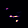
\includegraphics[width=0.12\textwidth]{resultats/LGD/sizes/size_mid2-init-pas=0.1_filtre=s-None.png}
&
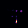
\includegraphics[width=0.12\textwidth]{resultats/LGD/sizes/size_mid1-init-pas=0.1_filtre=s-None.png}
&
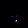
\includegraphics[width=0.12\textwidth]{resultats/LGD/sizes/size_small-init-pas=0.05_filtre=s-None.png}
&
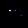
\includegraphics[width=0.12\textwidth]{resultats/LGD/sizes/size_mini-init-pas=0.01_filtre=s-None.png}

\\


&

\includegraphics[width=0.12\textwidth]{resultats/LGD/sizes/size_big-compatarget-s.png}
&

\includegraphics[width=0.12\textwidth]{resultats/LGD/sizes/size_mid2-compatarget-s.png}
&

\includegraphics[height=0.12\textwidth]{resultats/LGD/sizes/size_mid1-compatarget-s.png}
&

\includegraphics[width=0.12\textwidth]{resultats/LGD/sizes/size_small-compatarget-s.png}
&

\includegraphics[width=0.12\textwidth]{resultats/LGD/sizes/size_mini-compatarget-s.png}

\\


&

\includegraphics[width=0.12\textwidth]{resultats/LGD/sizes/size_big-guess-pas=0.1_filtre=s-None.png}
&

\includegraphics[width=0.12\textwidth]{resultats/LGD/sizes/size_mid2-guess-pas=0.1_filtre=s-None.png}
&
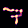
\includegraphics[width=0.12\textwidth]{resultats/LGD/sizes/size_mid1-guess-pas=0.1_filtre=s-None.png}
&
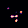
\includegraphics[width=0.12\textwidth]{resultats/LGD/sizes/size_small-guess-pas=0.05_filtre=s-None.png}
&
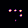
\includegraphics[width=0.12\textwidth]{resultats/LGD/sizes/size_mini-guess-pas=0.01_filtre=s-None.png}

\\ \\



\multicolumn{2}{c}{Loss}  &  \multicolumn{4}{c}{PSNR{\color{white}bbbb}}

\\

\multicolumn{2}{c}{% This file was created with tikzplotlib v0.10.1.
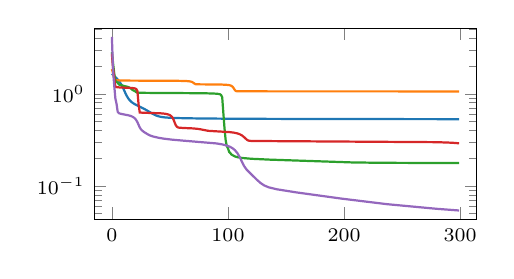
\begin{tikzpicture}

\definecolor{crimson2143940}{RGB}{214,39,40}
\definecolor{darkgray176}{RGB}{176,176,176}
\definecolor{darkorange25512714}{RGB}{255,127,14}
\definecolor{forestgreen4416044}{RGB}{44,160,44}
\definecolor{mediumpurple148103189}{RGB}{148,103,189}
\definecolor{steelblue31119180}{RGB}{31,119,180}

\begin{axis}[compar,
	ymode=log]
\addplot [thick, steelblue31119180]
table {%
0 1.65230560302734
1 1.60967218875885
3 1.51980757713318
5 1.4276807308197
6 1.37903583049774
7 1.32599353790283
8 1.26667380332947
9 1.20057117938995
11 1.05875587463379
12 0.993848085403442
13 0.939155459403992
14 0.895524501800537
15 0.861427426338196
16 0.834641695022583
17 0.813176393508911
18 0.795508742332458
19 0.780535697937012
21 0.755721092224121
24 0.724630355834961
28 0.684367299079895
32 0.640052795410156
35 0.6075519323349
37 0.589563608169556
39 0.575842380523682
41 0.56618332862854
43 0.559664726257324
46 0.553641200065613
50 0.549216270446777
57 0.545149207115173
70 0.541172504425049
93 0.53755521774292
135 0.534475564956665
221 0.531806707382202
299 0.530493259429932
};
\addplot [thick, darkorange25512714]
table {%
0 1.85211646556854
1 1.67770111560822
2 1.46272897720337
3 1.41593718528748
4 1.40484702587128
5 1.39981067180634
7 1.39501214027405
10 1.39188122749329
16 1.38930439949036
32 1.38671922683716
55 1.38247323036194
61 1.37871134281158
64 1.3742892742157
66 1.36830806732178
67 1.36319196224213
68 1.3552680015564
69 1.34236979484558
70 1.32132458686829
71 1.292635679245
72 1.27158439159393
73 1.26629757881165
76 1.26518905162811
89 1.26179456710815
95 1.25753927230835
98 1.25268864631653
100 1.24624443054199
101 1.24075663089752
102 1.23218429088593
103 1.21773552894592
104 1.191610455513
105 1.1454873085022
106 1.09121680259705
107 1.06940352916718
108 1.06570613384247
111 1.06433713436127
144 1.06147050857544
275 1.06137251853943
299 1.06136870384216
};
\addplot [thick, forestgreen4416044]
table {%
0 2.84194612503052
1 2.15506029129028
2 1.66873693466187
3 1.38294208049774
5 1.31623303890228
6 1.26444888114929
7 1.24834167957306
9 1.23046517372131
11 1.20998632907867
13 1.19424068927765
14 1.18405818939209
15 1.1702915430069
16 1.15001618862152
17 1.1210218667984
18 1.09569573402405
19 1.08197319507599
20 1.06478106975555
21 1.0405730009079
22 1.02683997154236
25 1.02437090873718
35 1.02164471149445
77 1.01418256759644
85 1.00862324237823
89 1.00375008583069
91 0.999232292175293
92 0.9952312707901
93 0.988119006156921
94 0.972235679626465
95 0.91933798789978
96 0.616937160491943
97 0.421802282333374
98 0.312908411026001
99 0.270792961120605
100 0.255544066429138
101 0.234020471572876
102 0.227557420730591
103 0.219099283218384
106 0.209146738052368
108 0.20545756816864
112 0.201385498046875
120 0.197391390800476
136 0.193149089813232
207 0.180134654045105
232 0.178421974182129
299 0.177336454391479
};
\addplot [thick, crimson2143940]
table {%
0 2.71224212646484
1 1.89663374423981
2 1.51032817363739
3 1.19073891639709
4 1.18067479133606
6 1.17347884178162
9 1.16805064678192
17 1.15556478500366
19 1.1488208770752
20 1.14171743392944
21 1.12556207180023
22 1.0690438747406
23 0.763562440872192
24 0.626803040504456
26 0.623935461044312
42 0.614003896713257
45 0.609050154685974
47 0.603470325469971
49 0.593772172927856
50 0.585844755172729
51 0.574084281921387
52 0.555935382843018
53 0.527923822402954
54 0.490156412124634
55 0.456605553627014
56 0.438905239105225
57 0.431463479995728
58 0.428577065467834
61 0.426207780838013
70 0.421022057533264
74 0.416285991668701
77 0.410333037376404
83 0.396579504013062
88 0.392909526824951
101 0.38445782661438
105 0.37907612323761
108 0.372137427330017
110 0.364766120910645
112 0.353622436523438
114 0.337481260299683
116 0.319562911987305
117 0.313272714614868
118 0.309869647026062
120 0.30800199508667
132 0.30707573890686
280 0.298706293106079
293 0.294538974761963
299 0.290218830108643
};
\addplot [thick, mediumpurple148103189]
table {%
0 4.13749027252197
1 1.78226494789124
2 1.23609900474548
3 0.890265941619873
4 0.779228687286377
5 0.638609528541565
6 0.617340087890625
7 0.609525799751282
9 0.601629018783569
14 0.585130453109741
16 0.575769901275635
17 0.569563150405884
18 0.561703205108643
19 0.551372528076172
20 0.537355184555054
21 0.517969131469727
22 0.491822361946106
23 0.46056592464447
24 0.431907415390015
25 0.412346363067627
26 0.399762630462646
28 0.382634878158569
31 0.362732648849487
33 0.35280454158783
36 0.34282374382019
40 0.333760499954224
45 0.325755834579468
52 0.317875027656555
63 0.309140682220459
90 0.289501667022705
95 0.28264594078064
99 0.274349570274353
102 0.264988541603088
104 0.256195902824402
106 0.244262218475342
108 0.227995634078979
110 0.206859588623047
113 0.172638773918152
114 0.163624286651611
116 0.150722026824951
119 0.13795006275177
125 0.116512775421143
128 0.107834815979004
131 0.10168719291687
135 0.0967668294906616
142 0.0921484231948853
159 0.0851820707321167
198 0.0729167461395264
237 0.0635035037994385
279 0.0566712617874146
299 0.0542340278625488
};
\end{axis}

\end{tikzpicture}
}
&
\multicolumn{4}{c}{% This file was created with tikzplotlib v0.10.1.
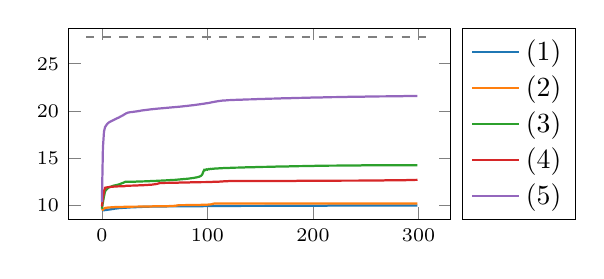
\begin{tikzpicture}

\definecolor{crimson2143940}{RGB}{214,39,40}
\definecolor{darkgray176}{RGB}{176,176,176}
\definecolor{darkorange25512714}{RGB}{255,127,14}
\definecolor{forestgreen4416044}{RGB}{44,160,44}
\definecolor{mediumpurple148103189}{RGB}{148,103,189}
\definecolor{steelblue31119180}{RGB}{31,119,180}

\begin{axis}[compar, legend pos=outer north east]
\addplot [thick, steelblue31119180]
table {%
0 9.43000030517578
1 9.44999980926514
3 9.47000026702881
4 9.48999977111816
5 9.5
6 9.52000045776367
7 9.52999973297119
9 9.56999969482422
10 9.57999992370605
13 9.64000034332275
15 9.65999984741211
16 9.68000030517578
18 9.69999980926514
19 9.69999980926514
22 9.72999954223633
23 9.72999954223633
25 9.75
26 9.75
27 9.76000022888184
28 9.76000022888184
29 9.77000045776367
30 9.77000045776367
31 9.77999973297119
32 9.77999973297119
34 9.80000019073486
35 9.80000019073486
36 9.8100004196167
38 9.8100004196167
39 9.81999969482422
40 9.81999969482422
41 9.82999992370605
44 9.82999992370605
45 9.84000015258789
48 9.84000015258789
49 9.85000038146973
54 9.85000038146973
55 9.85999965667725
61 9.85999965667725
62 9.86999988555908
71 9.86999988555908
72 9.88000011444092
82 9.88000011444092
83 9.89000034332275
96 9.89000034332275
97 9.89999961853027
112 9.89999961853027
113 9.90999984741211
131 9.90999984741211
132 9.92000007629395
154 9.92000007629395
155 9.93000030517578
181 9.93000030517578
182 9.9399995803833
213 9.9399995803833
214 9.94999980926514
251 9.94999980926514
252 9.96000003814697
295 9.96000003814697
296 9.97000026702881
299 9.97000026702881
};
\addlegendentry{$(1)$}
\addplot [thick, darkorange25512714]
table {%
0 9.4399995803833
1 9.52000045776367
2 9.64000034332275
3 9.6899995803833
4 9.72000026702881
5 9.72999954223633
6 9.75
7 9.76000022888184
8 9.76000022888184
10 9.77999973297119
11 9.77999973297119
12 9.78999996185303
14 9.78999996185303
15 9.80000019073486
16 9.80000019073486
17 9.8100004196167
20 9.8100004196167
21 9.81999969482422
24 9.81999969482422
25 9.82999992370605
29 9.82999992370605
30 9.84000015258789
34 9.84000015258789
35 9.85000038146973
40 9.85000038146973
41 9.85999965667725
47 9.85999965667725
48 9.86999988555908
53 9.86999988555908
54 9.88000011444092
59 9.88000011444092
60 9.89000034332275
63 9.89000034332275
64 9.89999961853027
66 9.89999961853027
70 9.9399995803833
72 9.97999954223633
74 10
79 10
80 10.0100002288818
87 10.0100002288818
88 10.0200004577637
93 10.0200004577637
94 10.0299997329712
97 10.0299997329712
98 10.039999961853
99 10.039999961853
103 10.0799999237061
104 10.1000003814697
106 10.1599998474121
107 10.1700000762939
170 10.1700000762939
171 10.1800003051758
299 10.1800003051758
};
\addlegendentry{$(2)$}
\addplot [thick, forestgreen4416044]
table {%
0 9.60999965667725
1 10.289999961853
2 10.9300003051758
3 11.4499998092651
4 11.6199998855591
5 11.710000038147
6 11.8199996948242
7 11.9099998474121
8 11.9399995803833
11 12.0600004196167
12 12.0900001525879
13 12.1099996566772
14 12.1400003433228
15 12.1599998474121
16 12.1899995803833
17 12.2299995422363
18 12.2799997329712
20 12.3599996566772
21 12.4099998474121
22 12.4700002670288
23 12.4799995422363
27 12.4799995422363
28 12.4899997711182
32 12.4899997711182
33 12.5
35 12.5
36 12.5100002288818
38 12.5100002288818
39 12.5200004577637
40 12.5200004577637
41 12.5299997329712
43 12.5299997329712
44 12.539999961853
45 12.539999961853
46 12.5500001907349
47 12.5500001907349
48 12.5600004196167
49 12.5600004196167
50 12.5699996948242
51 12.5699996948242
52 12.5799999237061
53 12.5799999237061
55 12.6000003814697
56 12.6000003814697
57 12.6099996566772
58 12.6099996566772
59 12.6199998855591
60 12.6199998855591
62 12.6400003433228
63 12.6400003433228
65 12.6599998474121
66 12.6599998474121
68 12.6800003051758
69 12.6800003051758
82 12.8100004196167
83 12.8299999237061
84 12.8400001525879
85 12.8599996566772
86 12.8699998855591
90 12.9499998092651
92 13.0100002288818
93 13.0500001907349
94 13.1199998855591
95 13.2299995422363
96 13.5100002288818
97 13.75
98 13.7200002670288
99 13.8000001907349
100 13.7600002288818
101 13.8299999237061
102 13.8100004196167
103 13.8500003814697
104 13.8400001525879
105 13.8699998855591
106 13.8599996566772
107 13.8800001144409
108 13.8800001144409
109 13.8900003433228
110 13.8900003433228
111 13.9099998474121
112 13.9099998474121
113 13.9200000762939
114 13.9200000762939
115 13.9300003051758
117 13.9300003051758
118 13.9399995803833
119 13.9399995803833
120 13.9499998092651
121 13.9499998092651
122 13.960000038147
124 13.960000038147
125 13.9700002670288
126 13.9700002670288
127 13.9799995422363
129 13.9799995422363
130 13.9899997711182
132 13.9899997711182
133 14
135 14
136 14.0100002288818
138 14.0100002288818
139 14.0200004577637
142 14.0200004577637
143 14.0299997329712
145 14.0299997329712
146 14.039999961853
149 14.039999961853
150 14.0500001907349
152 14.0500001907349
153 14.0600004196167
156 14.0600004196167
157 14.0699996948242
160 14.0699996948242
161 14.0799999237061
164 14.0799999237061
165 14.0900001525879
168 14.0900001525879
169 14.1000003814697
172 14.1000003814697
173 14.1099996566772
177 14.1099996566772
178 14.1199998855591
181 14.1199998855591
182 14.1300001144409
186 14.1300001144409
187 14.1400003433228
190 14.1400003433228
191 14.1499996185303
195 14.1499996185303
196 14.1599998474121
201 14.1599998474121
202 14.1700000762939
207 14.1700000762939
208 14.1800003051758
214 14.1800003051758
215 14.1899995803833
222 14.1899995803833
223 14.1999998092651
232 14.1999998092651
233 14.210000038147
245 14.210000038147
246 14.2200002670288
262 14.2200002670288
263 14.2299995422363
281 14.2299995422363
282 14.2399997711182
299 14.2399997711182
};
\addlegendentry{$(3)$}
\addplot [thick, crimson2143940]
table {%
0 9.85000038146973
1 10.7600002288818
2 11.4700002670288
3 11.8400001525879
4 11.8699998855591
5 11.8900003433228
6 11.8999996185303
7 11.9200000762939
12 11.9700002670288
13 11.9700002670288
15 11.9899997711182
16 11.9899997711182
17 12
18 12
19 12.0100002288818
21 12.0100002288818
22 12.0200004577637
23 12.0600004196167
27 12.0600004196167
28 12.0699996948242
29 12.0699996948242
30 12.0799999237061
32 12.0799999237061
33 12.0900001525879
34 12.0900001525879
35 12.1000003814697
36 12.1000003814697
37 12.1099996566772
38 12.1099996566772
39 12.1199998855591
40 12.1199998855591
42 12.1400003433228
43 12.1400003433228
45 12.1599998474121
46 12.1599998474121
48 12.1800003051758
49 12.1999998092651
50 12.210000038147
52 12.25
55 12.3400001525879
56 12.3500003814697
59 12.3500003814697
60 12.3599996566772
63 12.3599996566772
64 12.3699998855591
68 12.3699998855591
69 12.3800001144409
72 12.3800001144409
73 12.3900003433228
76 12.3900003433228
77 12.3999996185303
80 12.3999996185303
81 12.4099998474121
83 12.4099998474121
84 12.4200000762939
88 12.4200000762939
89 12.4300003051758
93 12.4300003051758
94 12.4399995803833
98 12.4399995803833
99 12.4499998092651
101 12.4499998092651
102 12.460000038147
104 12.460000038147
105 12.4700002670288
107 12.4700002670288
108 12.4799995422363
109 12.4799995422363
110 12.4899997711182
111 12.4899997711182
112 12.5
113 12.5
116 12.5299997329712
117 12.5299997329712
118 12.539999961853
119 12.539999961853
120 12.5500001907349
136 12.5500001907349
137 12.5600004196167
160 12.5600004196167
161 12.5699996948242
184 12.5699996948242
185 12.5799999237061
207 12.5799999237061
208 12.5900001525879
226 12.5900001525879
227 12.6000003814697
243 12.6000003814697
244 12.6099996566772
257 12.6099996566772
258 12.6199998855591
267 12.6199998855591
268 12.6300001144409
276 12.6300001144409
277 12.6400003433228
283 12.6400003433228
284 12.6499996185303
288 12.6499996185303
289 12.6599998474121
292 12.6599998474121
293 12.6700000762939
296 12.6700000762939
297 12.6800003051758
298 12.6800003051758
299 12.6899995803833
};
\addlegendentry{$(4)$}
\addplot [thick, mediumpurple148103189]
table {%
0 10.3500003814697
1 16.1200008392334
2 17.7999992370605
3 18.2800006866455
4 18.4400005340576
5 18.6100006103516
6 18.7099990844727
7 18.7999992370605
9 18.9200000762939
10 18.9699993133545
11 19.0300006866455
12 19.0799999237061
13 19.1399993896484
14 19.1900005340576
15 19.25
16 19.2900009155273
17 19.3600006103516
18 19.4099998474121
19 19.4799995422363
20 19.5300006866455
21 19.6100006103516
22 19.6700000762939
23 19.7399997711182
24 19.7800006866455
25 19.8299999237061
26 19.8400001525879
27 19.8700008392334
28 19.8700008392334
29 19.8899993896484
30 19.8999996185303
31 19.9200000762939
32 19.9300003051758
33 19.9500007629395
34 19.9599990844727
35 19.9899997711182
36 20
37 20.0300006866455
38 20.0400009155273
39 20.0599994659424
40 20.0699996948242
41 20.0900001525879
42 20.1000003814697
43 20.1200008392334
44 20.1299991607666
45 20.1499996185303
48 20.1800003051758
49 20.2000007629395
50 20.2000007629395
51 20.2199993133545
76 20.4699993133545
77 20.4899997711182
81 20.5300006866455
82 20.5499992370605
84 20.5699996948242
85 20.5900001525879
87 20.6100006103516
88 20.6299991607666
89 20.6399993896484
90 20.6599998474121
91 20.6700000762939
92 20.6900005340576
93 20.7000007629395
95 20.7399997711182
96 20.75
99 20.8099994659424
100 20.8199996948242
103 20.8799991607666
104 20.9099998474121
111 21.0499992370605
113 21.0699996948242
114 21.0900001525879
116 21.1100006103516
117 21.1100006103516
120 21.1399993896484
121 21.1399993896484
122 21.1499996185303
123 21.1499996185303
124 21.1599998474121
125 21.1599998474121
126 21.1700000762939
127 21.1700000762939
128 21.1800003051758
130 21.1800003051758
131 21.1900005340576
133 21.1900005340576
134 21.2000007629395
135 21.2000007629395
136 21.2099990844727
138 21.2099990844727
139 21.2199993133545
141 21.2199993133545
142 21.2299995422363
143 21.2299995422363
144 21.2399997711182
146 21.2399997711182
147 21.25
149 21.25
150 21.2600002288818
152 21.2600002288818
153 21.2700004577637
154 21.2700004577637
155 21.2800006866455
157 21.2800006866455
158 21.2900009155273
160 21.2900009155273
161 21.2999992370605
163 21.2999992370605
164 21.3099994659424
166 21.3099994659424
167 21.3199996948242
169 21.3199996948242
170 21.3299999237061
172 21.3299999237061
173 21.3400001525879
176 21.3400001525879
177 21.3500003814697
179 21.3500003814697
180 21.3600006103516
182 21.3600006103516
183 21.3700008392334
186 21.3700008392334
187 21.3799991607666
189 21.3799991607666
190 21.3899993896484
193 21.3899993896484
194 21.3999996185303
197 21.3999996185303
198 21.4099998474121
201 21.4099998474121
202 21.4200000762939
205 21.4200000762939
206 21.4300003051758
209 21.4300003051758
210 21.4400005340576
213 21.4400005340576
214 21.4500007629395
217 21.4500007629395
218 21.4599990844727
222 21.4599990844727
223 21.4699993133545
227 21.4699993133545
228 21.4799995422363
232 21.4799995422363
233 21.4899997711182
238 21.4899997711182
239 21.5
243 21.5
244 21.5100002288818
249 21.5100002288818
250 21.5200004577637
255 21.5200004577637
256 21.5300006866455
262 21.5300006866455
263 21.5400009155273
269 21.5400009155273
270 21.5499992370605
277 21.5499992370605
278 21.5599994659424
285 21.5599994659424
286 21.5699996948242
294 21.5699996948242
295 21.5799999237061
299 21.5799999237061
};
\addlegendentry{$(5)$}
\addplot [thick, gray, dashed]
table {%
-14.95 27.8502388000488
313.95 27.8502388000488
};
\end{axis}

\end{tikzpicture}
}
\end{tabular}
    %\includegraphics[width=1.\textwidth]{../resultats/LGD/differentes initialisation/inits-s_multiplot.png}
    \caption{En première lignes différentes initialisation avec en dessous le résultats de la LGD après 300 itérations -- sans filtre passe-bas}
    \label{fig:LGDinits}
\end{figure}

\begin{figure}[H]\centering
    \begin{tabular}{c c c c c c}
Target  &  $(1)$  &  $(2)$  &  $(3)$  &  $(4)$

\\

\multirow{2}{0.3\textwidth}[0.125\textwidth]{
\includegraphics[width=0.3\textwidth]{resultats/LGD/inits/inits-target-g.png}}
&

\includegraphics[width=0.15\textwidth]{resultats/LGD/inits/inits_1-init-pas=0.25_filtre=g-0.6.png}
&

\includegraphics[width=0.15\textwidth]{resultats/LGD/inits/inits_2-init-pas=0.25_filtre=g-0.6.png}
&

\includegraphics[width=0.15\textwidth]{resultats/LGD/inits/inits_3-init-pas=0.25_filtre=g-0.6.png}
&

\includegraphics[width=0.15\textwidth]{resultats/LGD/inits/inits_4-init-pas=0.25_filtre=g-0.6.png}

\\


&

\includegraphics[width=0.15\textwidth]{resultats/LGD/inits/inits_1-guess-pas=0.25_filtre=g-0.6.png}
&

\includegraphics[width=0.15\textwidth]{resultats/LGD/inits/inits_2-guess-pas=0.25_filtre=g-0.6.png}
&

\includegraphics[width=0.15\textwidth]{resultats/LGD/inits/inits_3-guess-pas=0.25_filtre=g-0.6.png}
&

\includegraphics[width=0.15\textwidth]{resultats/LGD/inits/inits_4-guess-pas=0.25_filtre=g-0.6.png}

\\ \\



\multicolumn{2}{c}{Loss}  &  \multicolumn{3}{c}{PSNR{\color{white}bbbb}}

\\

\multicolumn{2}{c}{% This file was created with tikzplotlib v0.10.1.
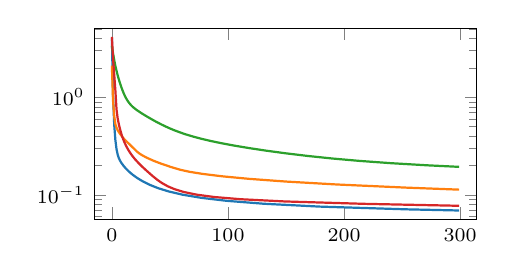
\begin{tikzpicture}

\definecolor{crimson2143940}{RGB}{214,39,40}
\definecolor{darkgray176}{RGB}{176,176,176}
\definecolor{darkorange25512714}{RGB}{255,127,14}
\definecolor{forestgreen4416044}{RGB}{44,160,44}
\definecolor{steelblue31119180}{RGB}{31,119,180}

\begin{axis}[compar,
	ymode=log]
\addplot [thick, steelblue31119180]
table {%
0 4.09705591201782
1 1.0397447347641
2 0.525999307632446
3 0.36544942855835
4 0.294240236282349
5 0.258731842041016
6 0.23837411403656
7 0.2248694896698
8 0.214669942855835
10 0.199013829231262
12 0.18678867816925
15 0.172265887260437
18 0.160792350769043
22 0.148674130439758
27 0.136995673179626
33 0.126390695571899
40 0.117159008979797
49 0.108532667160034
61 0.100532412528992
77 0.0933989286422729
99 0.0870349407196045
131 0.0812307596206665
179 0.0759825706481934
254 0.0712192058563232
299 0.0692975521087646
};
\addplot [thick, darkorange25512714]
table {%
0 2.11676383018494
1 0.9190913438797
2 0.643004417419434
3 0.532035350799561
4 0.487879872322083
5 0.460638880729675
6 0.440029859542847
7 0.422846078872681
9 0.393353462219238
11 0.368957042694092
13 0.349978923797607
22 0.275432348251343
24 0.264232397079468
27 0.25137186050415
31 0.237775444984436
36 0.22367525100708
42 0.210012912750244
51 0.193120121955872
59 0.180989027023315
67 0.172550797462463
78 0.164394378662109
95 0.155235648155212
118 0.146238088607788
150 0.137122750282288
194 0.127958059310913
254 0.118792176246643
299 0.113348960876465
};
\addplot [thick, forestgreen4416044]
table {%
0 3.37779760360718
1 2.81990122795105
2 2.4142701625824
3 2.10492038726807
4 1.86983335018158
5 1.67920529842377
6 1.52351367473602
7 1.3948290348053
8 1.2856605052948
9 1.19226157665253
10 1.11291658878326
11 1.04617238044739
12 0.990375518798828
13 0.94380521774292
14 0.904836654663086
15 0.872018575668335
16 0.844097495079041
17 0.820020079612732
18 0.798925280570984
19 0.780128955841064
21 0.747454047203064
23 0.719166994094849
25 0.693710803985596
28 0.659082055091858
31 0.627551555633545
34 0.598529100418091
38 0.563355803489685
42 0.532020330429077
46 0.504339337348938
50 0.480038523674011
54 0.458757042884827
59 0.435793519020081
64 0.416170716285706
70 0.396113634109497
77 0.376400947570801
85 0.357464551925659
94 0.339470624923706
105 0.320858478546143
118 0.30225658416748
133 0.284092664718628
150 0.266751885414124
169 0.250633358955383
190 0.236100435256958
213 0.223376154899597
240 0.211698055267334
272 0.201091408729553
299 0.194014668464661
};
\addplot [thick, crimson2143940]
table {%
0 4.15872049331665
1 2.48774647712708
2 1.71559143066406
3 1.18148231506348
4 0.74964714050293
5 0.606518745422363
6 0.529028296470642
7 0.472540497779846
8 0.428424477577209
9 0.393683195114136
10 0.365716695785522
11 0.342551231384277
12 0.322939038276672
13 0.306079387664795
14 0.291416645050049
16 0.267123222351074
18 0.247718811035156
20 0.231697797775269
23 0.211907505989075
26 0.195417284965515
30 0.176599979400635
35 0.156593918800354
39 0.143312335014343
43 0.132702112197876
48 0.12282931804657
54 0.114545702934265
62 0.10715639591217
73 0.100697159767151
88 0.0952965021133423
111 0.0903933048248291
149 0.0857839584350586
217 0.0811049938201904
299 0.0774440765380859
};

\end{axis}

\end{tikzpicture}
}
&
\multicolumn{3}{c}{% This file was created with tikzplotlib v0.10.1.
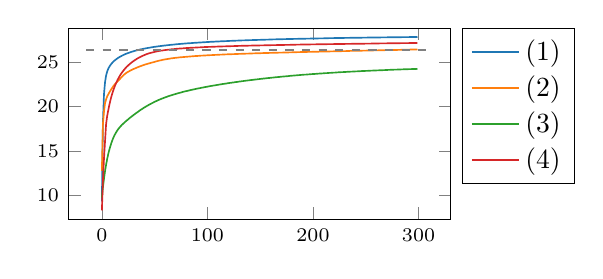
\begin{tikzpicture}

\definecolor{crimson2143940}{RGB}{214,39,40}
\definecolor{darkgray176}{RGB}{176,176,176}
\definecolor{darkorange25512714}{RGB}{255,127,14}
\definecolor{forestgreen4416044}{RGB}{44,160,44}
\definecolor{steelblue31119180}{RGB}{31,119,180}

\begin{axis}[compar, legend pos=outer north east]
\addplot [semithick, steelblue31119180]
table {%
0 9.34000015258789
1 18.2600002288818
2 21.3700008392334
3 22.7199993133545
4 23.4599990844727
5 23.8999996185303
6 24.2099990844727
7 24.4300003051758
8 24.6200008392334
9 24.7700004577637
10 24.9099998474121
11 25.0300006866455
12 25.1399993896484
15 25.4099998474121
16 25.4799995422363
17 25.5599994659424
21 25.7999992370605
24 25.9500007629395
29 26.1499996185303
30 26.1800003051758
31 26.2199993133545
37 26.3999996185303
38 26.4200000762939
39 26.4500007629395
41 26.4899997711182
42 26.5200004577637
50 26.6800003051758
51 26.6900005340576
53 26.7299995422363
54 26.7399997711182
55 26.7600002288818
56 26.7700004577637
57 26.7900009155273
58 26.7999992370605
59 26.8199996948242
61 26.8400001525879
62 26.8600006103516
64 26.8799991607666
65 26.8999996185303
69 26.9400005340576
70 26.9599990844727
82 27.0799999237061
83 27.0799999237061
88 27.1299991607666
89 27.1299991607666
93 27.1700000762939
94 27.1700000762939
96 27.1900005340576
97 27.1900005340576
100 27.2199993133545
101 27.2199993133545
103 27.2399997711182
104 27.2399997711182
105 27.25
106 27.25
108 27.2700004577637
109 27.2700004577637
110 27.2800006866455
111 27.2800006866455
113 27.2999992370605
114 27.2999992370605
115 27.3099994659424
116 27.3099994659424
117 27.3199996948242
118 27.3199996948242
119 27.3299999237061
120 27.3299999237061
121 27.3400001525879
122 27.3400001525879
123 27.3500003814697
124 27.3500003814697
125 27.3600006103516
126 27.3600006103516
127 27.3700008392334
128 27.3700008392334
129 27.3799991607666
130 27.3799991607666
131 27.3899993896484
132 27.3899993896484
133 27.3999996185303
135 27.3999996185303
136 27.4099998474121
137 27.4099998474121
138 27.4200000762939
139 27.4200000762939
140 27.4300003051758
142 27.4300003051758
143 27.4400005340576
144 27.4400005340576
145 27.4500007629395
147 27.4500007629395
148 27.4599990844727
150 27.4599990844727
151 27.4699993133545
153 27.4699993133545
154 27.4799995422363
155 27.4799995422363
156 27.4899997711182
158 27.4899997711182
159 27.5
161 27.5
162 27.5100002288818
164 27.5100002288818
165 27.5200004577637
168 27.5200004577637
169 27.5300006866455
171 27.5300006866455
172 27.5400009155273
174 27.5400009155273
175 27.5499992370605
178 27.5499992370605
179 27.5599994659424
181 27.5599994659424
182 27.5699996948242
185 27.5699996948242
186 27.5799999237061
189 27.5799999237061
190 27.5900001525879
193 27.5900001525879
194 27.6000003814697
197 27.6000003814697
198 27.6100006103516
201 27.6100006103516
202 27.6200008392334
205 27.6200008392334
206 27.6299991607666
210 27.6299991607666
211 27.6399993896484
214 27.6399993896484
215 27.6499996185303
219 27.6499996185303
220 27.6599998474121
224 27.6599998474121
225 27.6700000762939
229 27.6700000762939
230 27.6800003051758
234 27.6800003051758
235 27.6900005340576
240 27.6900005340576
241 27.7000007629395
246 27.7000007629395
247 27.7099990844727
251 27.7099990844727
252 27.7199993133545
257 27.7199993133545
258 27.7299995422363
264 27.7299995422363
265 27.7399997711182
270 27.7399997711182
271 27.75
277 27.75
278 27.7600002288818
284 27.7600002288818
285 27.7700004577637
291 27.7700004577637
292 27.7800006866455
298 27.7800006866455
299 27.7900009155273
};
\addlegendentry{$(1)$}
\addplot [semithick, darkorange25512714]
table {%
0 12.7600002288818
1 18.0300006866455
2 19.4099998474121
3 20.3700008392334
4 20.7800006866455
5 21.1100006103516
7 21.5499992370605
8 21.75
9 21.9400005340576
10 22.1200008392334
11 22.2900009155273
12 22.4400005340576
13 22.5799999237061
16 22.9400005340576
17 23.0699996948242
18 23.1900005340576
19 23.3199996948242
20 23.4400005340576
21 23.5499992370605
22 23.6499996185303
23 23.7399997711182
24 23.8199996948242
25 23.8899993896484
26 23.9500007629395
27 24.0200004577637
28 24.0799999237061
29 24.1299991607666
30 24.1900005340576
36 24.4899997711182
42 24.7299995422363
43 24.7600002288818
44 24.7999992370605
46 24.8600006103516
47 24.8999996185303
50 24.9899997711182
51 25.0300006866455
55 25.1499996185303
56 25.1700000762939
58 25.2299995422363
66 25.3899993896484
67 25.3999996185303
68 25.4200000762939
69 25.4300003051758
70 25.4500007629395
72 25.4699993133545
73 25.4899997711182
89 25.6499996185303
90 25.6499996185303
94 25.6900005340576
95 25.6900005340576
97 25.7099990844727
98 25.7099990844727
100 25.7299995422363
101 25.7299995422363
103 25.75
104 25.75
105 25.7600002288818
106 25.7600002288818
108 25.7800006866455
109 25.7800006866455
110 25.7900009155273
111 25.7900009155273
112 25.7999992370605
113 25.7999992370605
115 25.8199996948242
116 25.8199996948242
117 25.8299999237061
118 25.8299999237061
119 25.8400001525879
120 25.8400001525879
121 25.8500003814697
123 25.8500003814697
124 25.8600006103516
125 25.8600006103516
126 25.8700008392334
127 25.8700008392334
128 25.8799991607666
129 25.8799991607666
130 25.8899993896484
132 25.8899993896484
133 25.8999996185303
134 25.8999996185303
135 25.9099998474121
136 25.9099998474121
137 25.9200000762939
139 25.9200000762939
140 25.9300003051758
142 25.9300003051758
143 25.9400005340576
144 25.9400005340576
145 25.9500007629395
147 25.9500007629395
148 25.9599990844727
150 25.9599990844727
151 25.9699993133545
152 25.9699993133545
153 25.9799995422363
155 25.9799995422363
156 25.9899997711182
158 25.9899997711182
159 26
161 26
162 26.0100002288818
164 26.0100002288818
165 26.0200004577637
167 26.0200004577637
168 26.0300006866455
171 26.0300006866455
172 26.0400009155273
174 26.0400009155273
175 26.0499992370605
177 26.0499992370605
178 26.0599994659424
180 26.0599994659424
181 26.0699996948242
184 26.0699996948242
185 26.0799999237061
187 26.0799999237061
188 26.0900001525879
191 26.0900001525879
192 26.1000003814697
194 26.1000003814697
195 26.1100006103516
198 26.1100006103516
199 26.1200008392334
201 26.1200008392334
202 26.1299991607666
205 26.1299991607666
206 26.1399993896484
208 26.1399993896484
209 26.1499996185303
212 26.1499996185303
213 26.1599998474121
216 26.1599998474121
217 26.1700000762939
219 26.1700000762939
220 26.1800003051758
223 26.1800003051758
224 26.1900005340576
227 26.1900005340576
228 26.2000007629395
231 26.2000007629395
232 26.2099990844727
234 26.2099990844727
235 26.2199993133545
238 26.2199993133545
239 26.2299995422363
242 26.2299995422363
243 26.2399997711182
246 26.2399997711182
247 26.25
250 26.25
251 26.2600002288818
253 26.2600002288818
254 26.2700004577637
257 26.2700004577637
258 26.2800006866455
261 26.2800006866455
262 26.2900009155273
265 26.2900009155273
266 26.2999992370605
268 26.2999992370605
269 26.3099994659424
272 26.3099994659424
273 26.3199996948242
276 26.3199996948242
277 26.3299999237061
280 26.3299999237061
281 26.3400001525879
283 26.3400001525879
284 26.3500003814697
287 26.3500003814697
288 26.3600006103516
291 26.3600006103516
292 26.3700008392334
295 26.3700008392334
296 26.3799991607666
298 26.3799991607666
299 26.3899993896484
};
\addlegendentry{$(2)$}
\addplot [semithick, forestgreen4416044]
table {%
0 9.77999973297119
1 10.9300003051758
2 11.8999996185303
3 12.7399997711182
4 13.460000038147
5 14.0900001525879
6 14.6400003433228
7 15.1099996566772
8 15.5299997329712
9 15.8999996185303
10 16.2299995422363
11 16.5200004577637
12 16.7700004577637
13 16.9899997711182
14 17.1900005340576
15 17.3700008392334
16 17.5300006866455
17 17.6700000762939
19 17.9300003051758
22 18.2600002288818
27 18.7600002288818
32 19.2099990844727
33 19.2900009155273
34 19.3799991607666
35 19.4599990844727
36 19.5499992370605
37 19.6299991607666
38 19.7000007629395
40 19.8600006103516
45 20.2099990844727
51 20.5699996948242
52 20.6200008392334
53 20.6800003051758
57 20.8799991607666
58 20.9200000762939
59 20.9699993133545
61 21.0499992370605
62 21.1000003814697
65 21.2199993133545
66 21.25
68 21.3299999237061
69 21.3600006103516
70 21.3999996185303
71 21.4300003051758
72 21.4699993133545
75 21.5599994659424
76 21.6000003814697
79 21.6900005340576
80 21.7099990844727
84 21.8299999237061
85 21.8500003814697
87 21.9099998474121
88 21.9300003051758
89 21.9599990844727
90 21.9799995422363
91 22.0100002288818
93 22.0499992370605
94 22.0799999237061
96 22.1200008392334
97 22.1499996185303
100 22.2099990844727
101 22.2399997711182
115 22.5200004577637
116 22.5300006866455
121 22.6299991607666
122 22.6399993896484
124 22.6800003051758
125 22.6900005340576
127 22.7299995422363
128 22.7399997711182
130 22.7800006866455
131 22.7900009155273
133 22.8299999237061
134 22.8400001525879
135 22.8600006103516
136 22.8700008392334
137 22.8899993896484
138 22.8999996185303
139 22.9200000762939
140 22.9300003051758
141 22.9500007629395
142 22.9599990844727
143 22.9799995422363
144 22.9899997711182
145 23.0100002288818
147 23.0300006866455
148 23.0499992370605
149 23.0599994659424
150 23.0799999237061
152 23.1000003814697
153 23.1200008392334
155 23.1399993896484
156 23.1599998474121
159 23.1900005340576
160 23.2099990844727
163 23.2399997711182
164 23.2600002288818
168 23.2999992370605
169 23.3199996948242
177 23.3999996185303
178 23.4200000762939
192 23.5599994659424
193 23.5599994659424
201 23.6399993896484
202 23.6399993896484
207 23.6900005340576
208 23.6900005340576
212 23.7299995422363
213 23.7299995422363
216 23.7600002288818
217 23.7600002288818
220 23.7900009155273
221 23.7900009155273
224 23.8199996948242
225 23.8199996948242
227 23.8400001525879
228 23.8400001525879
230 23.8600006103516
231 23.8600006103516
233 23.8799991607666
234 23.8799991607666
236 23.8999996185303
237 23.8999996185303
238 23.9099998474121
239 23.9099998474121
241 23.9300003051758
242 23.9300003051758
243 23.9400005340576
244 23.9400005340576
246 23.9599990844727
247 23.9599990844727
248 23.9699993133545
249 23.9699993133545
250 23.9799995422363
251 23.9799995422363
253 24
254 24
255 24.0100002288818
256 24.0100002288818
257 24.0200004577637
258 24.0200004577637
259 24.0300006866455
260 24.0300006866455
261 24.0400009155273
262 24.0400009155273
263 24.0499992370605
264 24.0499992370605
265 24.0599994659424
266 24.0599994659424
267 24.0699996948242
268 24.0699996948242
269 24.0799999237061
270 24.0799999237061
271 24.0900001525879
272 24.0900001525879
273 24.1000003814697
274 24.1000003814697
275 24.1100006103516
276 24.1100006103516
277 24.1200008392334
279 24.1200008392334
280 24.1299991607666
281 24.1299991607666
282 24.1399993896484
283 24.1399993896484
284 24.1499996185303
285 24.1499996185303
286 24.1599998474121
288 24.1599998474121
289 24.1700000762939
290 24.1700000762939
291 24.1800003051758
293 24.1800003051758
294 24.1900005340576
295 24.1900005340576
296 24.2000007629395
298 24.2000007629395
299 24.2099990844727
};
\addlegendentry{$(3)$}
\addplot [semithick, crimson2143940]
table {%
0 8.32999992370605
1 11.6999998092651
2 14.1499996185303
3 16.1100006103516
4 18.0300006866455
5 18.9099998474121
6 19.5400009155273
7 20.1200008392334
8 20.6399993896484
9 21.1000003814697
10 21.5
11 21.8600006103516
12 22.1900005340576
13 22.4799995422363
14 22.75
15 23
16 23.2199993133545
17 23.4300003051758
18 23.6200008392334
19 23.7900009155273
20 23.9500007629395
21 24.1000003814697
22 24.2399997711182
23 24.3700008392334
24 24.4899997711182
26 24.7099990844727
28 24.9099998474121
29 25
30 25.0799999237061
31 25.1700000762939
32 25.2399997711182
33 25.3199996948242
35 25.4599990844727
38 25.6399993896484
42 25.8400001525879
45 25.9599990844727
51 26.1399993896484
53 26.1800003051758
54 26.2099990844727
56 26.25
57 26.2600002288818
60 26.3199996948242
61 26.3299999237061
62 26.3500003814697
64 26.3700008392334
65 26.3899993896484
69 26.4300003051758
70 26.4500007629395
74 26.4899997711182
75 26.4899997711182
80 26.5400009155273
81 26.5400009155273
84 26.5699996948242
85 26.5699996948242
87 26.5900001525879
88 26.5900001525879
90 26.6100006103516
91 26.6100006103516
92 26.6200008392334
93 26.6200008392334
94 26.6299991607666
95 26.6299991607666
97 26.6499996185303
98 26.6499996185303
99 26.6599998474121
100 26.6599998474121
101 26.6700000762939
103 26.6700000762939
104 26.6800003051758
105 26.6800003051758
106 26.6900005340576
107 26.6900005340576
108 26.7000007629395
109 26.7000007629395
110 26.7099990844727
112 26.7099990844727
113 26.7199993133545
114 26.7199993133545
115 26.7299995422363
117 26.7299995422363
118 26.7399997711182
120 26.7399997711182
121 26.75
122 26.75
123 26.7600002288818
125 26.7600002288818
126 26.7700004577637
128 26.7700004577637
129 26.7800006866455
131 26.7800006866455
132 26.7900009155273
135 26.7900009155273
136 26.7999992370605
138 26.7999992370605
139 26.8099994659424
141 26.8099994659424
142 26.8199996948242
145 26.8199996948242
146 26.8299999237061
149 26.8299999237061
150 26.8400001525879
153 26.8400001525879
154 26.8500003814697
156 26.8500003814697
157 26.8600006103516
160 26.8600006103516
161 26.8700008392334
165 26.8700008392334
166 26.8799991607666
169 26.8799991607666
170 26.8899993896484
173 26.8899993896484
174 26.8999996185303
178 26.8999996185303
179 26.9099998474121
183 26.9099998474121
184 26.9200000762939
187 26.9200000762939
188 26.9300003051758
192 26.9300003051758
193 26.9400005340576
197 26.9400005340576
198 26.9500007629395
202 26.9500007629395
203 26.9599990844727
208 26.9599990844727
209 26.9699993133545
213 26.9699993133545
214 26.9799995422363
219 26.9799995422363
220 26.9899997711182
225 26.9899997711182
226 27
230 27
231 27.0100002288818
236 27.0100002288818
237 27.0200004577637
243 27.0200004577637
244 27.0300006866455
249 27.0300006866455
250 27.0400009155273
255 27.0400009155273
256 27.0499992370605
262 27.0499992370605
263 27.0599994659424
269 27.0599994659424
270 27.0699996948242
275 27.0699996948242
276 27.0799999237061
282 27.0799999237061
283 27.0900001525879
290 27.0900001525879
291 27.1000003814697
297 27.1000003814697
298 27.1100006103516
299 27.1100006103516
};
\addlegendentry{$(4)$}
\addplot [semithick, gray,  dashed]
table {%
-14.95 26.3238544464111
313.95 26.3238544464111
};
\end{axis}

\end{tikzpicture}
}
\end{tabular}
    %\includegraphics[width=1.\textwidth]{../resultats/LGD/differentes initialisation/inits-g_multiplot.png}
    \caption{En première lignes différentes initialisation avec en dessous le résultats de la LGD après 300 itérations --  avec passe-bas gaussien ($\sigma=0.5$)}
    \label{fig:LGDinitg}
\end{figure}

Il va de soit que le calcul de PSNR est à but purement indicatif et n'intervient pas dans la LGD elle-même. Les ligne en pointillé représentent PSNR$\big(\bf{x_0},f(\bf{x_0})\big)$, le PSNR entre la cible $\bf{x_0}$ est sa version auto-encodée.
Dans la première figure \textit{\ref{fig:LGDinits}} il n'y pas de filtre passe-bas (\ei $A=S$) et dans la seconde \textit{\ref{fig:LGDinitg}}, $C_{\bf{h}}$ est un filtre gaussien de paramètre $\sigma=0.6$ (voir section \ref{sec:forma2pb} pour un rappel sur $\sigma$).
\\
Les différentes initialisations sont les suivantes :
\begin{enumerate}[label=(\arabic*)]
    \item $\bf{u_0}=f_E(^tA\bf{y_0})$, la backprojection encodée de $\bf{y_0}$
    \item $\bf{u_0}=f_E(\bf{x_0})+e$, l'image cible encodée puis bruité (bruit uniforme sur $]-0.5,0.5[$)
    \item idem, avec un bruit gaussien d'écart-type $0.5$
    \item $\bf{u_0}=\bf{u}_{\text{rand}}$,  vecteur aléatoire de l'espace latent
\end{enumerate}

\noindent La première initialisation est la plus naturelle puisqu'elle utilise $^tA$, ce qui se rapproche le plus d'un inverse pour $A$ (voir figure \textit{\ref{fig:passebas-g}} et \textit{\ref{fig:passebas-g}} en annexe \ref{anx:gradF} pour les visuels) et de même pour $f_E$ par rapport à $f_D$. 
\\
Les initialisations $(2)$ et $(3)$ sont au voisinage de de la cible  pour voir à quel point il possible de s'éloigner de $\bf{x_0}$ tout en conservant la convergence de l'algorithme.
\\

Cela étant dit, le premier constat est que la méthode fonctionne et ceux même en partant d'une vecteur aléatoire.  Aussi, même s'il sont meilleurs avec un passe-bas, les résultats restent satisfaisant sans filtre. La structure très simple du jeu de données aide probablement sur ce point et il serait intéressant de voir si les différences avec/sans filtre sont plus marqués sur un jeu de données plus complexe comme Fashion-MNIST.
\\
De plus, les courbes de loss de la figure \textit{\ref{fig:LGDinitg}} suggèrent que le résultats pourrait être améliorer avec plus d'itération. Celles de la figure \textit{\ref{fig:LGDinits}} suggère une convergence mais comme  les courbes fond des saut, il possible que $g$ puisse encore diminuer en échappant à ces plateaux. On pourrait par exemple ajouter de l'inertie à la descente.
\\

Autre chose remarquable, le résultats $(4)$ est meilleur que le $(3)$ alors que l'initialisation du premier est plus éloigné de la cible que le second. Cela est dû à la façon dont est tiré $\bf{u}_{\text{rand}}$. Pour rester cohérent avec la structure des images, et le réseau $f$ (qui est se termine par des sigmoïdes), les coefficients de $\bf{u}_{\text{rand}}$ sont tirés suivant une loi uniforme sur $[0,1]$. et l'auto encodeur gère très mal les vecteurs à valeurs trop loin de l'intervalle $[0,1]$. 
\\

Pour le voir, dans la figure \textit{\ref{fig:LGDmultarg-g}} ci-dessous, les deux premières initialisations, $(1)$ et $(2)$, sont faites avec un vecteur aléatoires tirés suivant une loi uniforme. Les deux suivantes, $(3)$ et $(4)$, le sont suivant des lois normales d'écart-type respectif 1 et 5. 
\\
Il apparaît clairement que l'auto-encodeur se comporte mal avec des initialisations trop loin de $[0,1]$. \emph{blablabla il te faut les résultats pour avancer là}

\begin{figure}[H]\centering
    %\begin{tabular}{c c c c c c}
Target  &  $(1)$  &  $(2)$  &  $(3)$  &  $(4)$

\\

\multirow{2}{0.3\textwidth}[0.125\textwidth]{\includegraphics[width=0.3\textwidth]{../../resultats/LGD/inits/inits-target-pas=0.05_filtre=g-0.5.png}}
&
\includegraphics[width=0.15\textwidth]{../../resultats/LGD/inits/inits_1-init-pas=0.05_filtre=g-0.5.png}
&
\includegraphics[width=0.15\textwidth]{../../resultats/LGD/inits/inits_2-init-pas=0.05_filtre=g-0.5.png}
&
\includegraphics[width=0.15\textwidth]{../../resultats/LGD/inits/inits_3-init-pas=0.05_filtre=g-0.5.png}
&
\includegraphics[width=0.15\textwidth]{../../resultats/LGD/inits/inits_4-init-pas=0.05_filtre=g-0.5.png}

\\


&
\includegraphics[width=0.15\textwidth]{../../resultats/LGD/inits/inits_1-guess-pas=0.05_filtre=g-0.5.png}
&
\includegraphics[width=0.15\textwidth]{../../resultats/LGD/inits/inits_2-guess-pas=0.05_filtre=g-0.5.png}
&
\includegraphics[width=0.15\textwidth]{../../resultats/LGD/inits/inits_3-guess-pas=0.05_filtre=g-0.5.png}
&
\includegraphics[width=0.15\textwidth]{../../resultats/LGD/inits/inits_4-guess-pas=0.05_filtre=g-0.5.png}

\\ \\



\multicolumn{2}{c}{Loss}  &  \multicolumn{3}{c}{PSNR}

\\

\multicolumn{2}{c}{\input{../../resultats/LGD/inits/inits-Fs-pas=0.05_filtre=g-0.5}}
&
\multicolumn{3}{c}{\input{../../resultats/LGD/inits/inits-PSNRs-pas=0.05_filtre=g-0.5}}
\end{tabular}
    %\includegraphics[width=1.\textwidth]{resultats/LGD/inits/inits-s_multiplot.png}
    \caption{En première lignes différentes initialisation avec en dessous le résultats de la LGD après 150 itérations --- sans passe-bas}
    \label{fig:LGDmultarg-s}
\end{figure}
\begin{figure}[H]\centering
    %\includegraphics[width=1.\textwidth]{resultats/LGD/inits/inits-g_multiplot.png}
    \caption{En première lignes différentes initialisation avec en dessous le résultats de la LGD après 10 itérations ---  avec passe-bas gaussien ($\sigma=0.5$)}
    \label{fig:LGDmultarg-g}
\end{figure}




%\\ \\



\subsection{Variation de la qualité de mesure (e.i. $\bf{p}\times\bf{q}$)}

\begin{figure}[H]\centering
	\begin{tabular}{c c c c c c}
Target  &  $(1)$  &  $(2)$  &  $(3)$  &  $(4)$  &  $(5)$

\\

\multirow{3}{0.3\textwidth}[0.05\textwidth]{\includegraphics[width=0.3\textwidth]{resultats/LGD/sizes/size-target-s.png}}
&
\includegraphics[width=0.12\textwidth]{resultats/LGD/sizes/size_big-init-pas=0.1_filtre=s-None.png}
&
\includegraphics[width=0.12\textwidth]{resultats/LGD/sizes/size_mid2-init-pas=0.1_filtre=s-None.png}
&
\includegraphics[width=0.12\textwidth]{resultats/LGD/sizes/size_mid1-init-pas=0.1_filtre=s-None.png}
&
\includegraphics[width=0.12\textwidth]{resultats/LGD/sizes/size_small-init-pas=0.05_filtre=s-None.png}
&
\includegraphics[width=0.12\textwidth]{resultats/LGD/sizes/size_mini-init-pas=0.01_filtre=s-None.png}

\\


&
\includegraphics[width=0.12\textwidth]{resultats/LGD/sizes/size_big-compatarget-s.png}
&
\includegraphics[width=0.12\textwidth]{resultats/LGD/sizes/size_mid2-compatarget-s.png}
&
\includegraphics[height=0.12\textwidth]{resultats/LGD/sizes/size_mid1-compatarget-s.png}
&
\includegraphics[width=0.12\textwidth]{resultats/LGD/sizes/size_small-compatarget-s.png}
&
\includegraphics[width=0.12\textwidth]{resultats/LGD/sizes/size_mini-compatarget-s.png}

\\


&
\includegraphics[width=0.12\textwidth]{resultats/LGD/sizes/size_big-guess-pas=0.1_filtre=s-None.png}
&
\includegraphics[width=0.12\textwidth]{resultats/LGD/sizes/size_mid2-guess-pas=0.1_filtre=s-None.png}
&
\includegraphics[width=0.12\textwidth]{resultats/LGD/sizes/size_mid1-guess-pas=0.1_filtre=s-None.png}
&
\includegraphics[width=0.12\textwidth]{resultats/LGD/sizes/size_small-guess-pas=0.05_filtre=s-None.png}
&
\includegraphics[width=0.12\textwidth]{resultats/LGD/sizes/size_mini-guess-pas=0.01_filtre=s-None.png}

\\ \\



\multicolumn{2}{c}{Loss}  &  \multicolumn{4}{c}{PSNR{\color{white}bbbb}}

\\

\multicolumn{2}{c}{% This file was created with tikzplotlib v0.10.1.
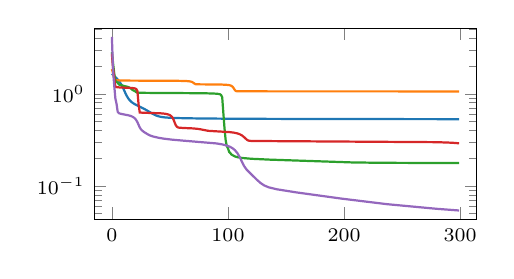
\begin{tikzpicture}

\definecolor{crimson2143940}{RGB}{214,39,40}
\definecolor{darkgray176}{RGB}{176,176,176}
\definecolor{darkorange25512714}{RGB}{255,127,14}
\definecolor{forestgreen4416044}{RGB}{44,160,44}
\definecolor{mediumpurple148103189}{RGB}{148,103,189}
\definecolor{steelblue31119180}{RGB}{31,119,180}

\begin{axis}[compar,
	ymode=log]
\addplot [thick, steelblue31119180]
table {%
0 1.65230560302734
1 1.60967218875885
3 1.51980757713318
5 1.4276807308197
6 1.37903583049774
7 1.32599353790283
8 1.26667380332947
9 1.20057117938995
11 1.05875587463379
12 0.993848085403442
13 0.939155459403992
14 0.895524501800537
15 0.861427426338196
16 0.834641695022583
17 0.813176393508911
18 0.795508742332458
19 0.780535697937012
21 0.755721092224121
24 0.724630355834961
28 0.684367299079895
32 0.640052795410156
35 0.6075519323349
37 0.589563608169556
39 0.575842380523682
41 0.56618332862854
43 0.559664726257324
46 0.553641200065613
50 0.549216270446777
57 0.545149207115173
70 0.541172504425049
93 0.53755521774292
135 0.534475564956665
221 0.531806707382202
299 0.530493259429932
};
\addplot [thick, darkorange25512714]
table {%
0 1.85211646556854
1 1.67770111560822
2 1.46272897720337
3 1.41593718528748
4 1.40484702587128
5 1.39981067180634
7 1.39501214027405
10 1.39188122749329
16 1.38930439949036
32 1.38671922683716
55 1.38247323036194
61 1.37871134281158
64 1.3742892742157
66 1.36830806732178
67 1.36319196224213
68 1.3552680015564
69 1.34236979484558
70 1.32132458686829
71 1.292635679245
72 1.27158439159393
73 1.26629757881165
76 1.26518905162811
89 1.26179456710815
95 1.25753927230835
98 1.25268864631653
100 1.24624443054199
101 1.24075663089752
102 1.23218429088593
103 1.21773552894592
104 1.191610455513
105 1.1454873085022
106 1.09121680259705
107 1.06940352916718
108 1.06570613384247
111 1.06433713436127
144 1.06147050857544
275 1.06137251853943
299 1.06136870384216
};
\addplot [thick, forestgreen4416044]
table {%
0 2.84194612503052
1 2.15506029129028
2 1.66873693466187
3 1.38294208049774
5 1.31623303890228
6 1.26444888114929
7 1.24834167957306
9 1.23046517372131
11 1.20998632907867
13 1.19424068927765
14 1.18405818939209
15 1.1702915430069
16 1.15001618862152
17 1.1210218667984
18 1.09569573402405
19 1.08197319507599
20 1.06478106975555
21 1.0405730009079
22 1.02683997154236
25 1.02437090873718
35 1.02164471149445
77 1.01418256759644
85 1.00862324237823
89 1.00375008583069
91 0.999232292175293
92 0.9952312707901
93 0.988119006156921
94 0.972235679626465
95 0.91933798789978
96 0.616937160491943
97 0.421802282333374
98 0.312908411026001
99 0.270792961120605
100 0.255544066429138
101 0.234020471572876
102 0.227557420730591
103 0.219099283218384
106 0.209146738052368
108 0.20545756816864
112 0.201385498046875
120 0.197391390800476
136 0.193149089813232
207 0.180134654045105
232 0.178421974182129
299 0.177336454391479
};
\addplot [thick, crimson2143940]
table {%
0 2.71224212646484
1 1.89663374423981
2 1.51032817363739
3 1.19073891639709
4 1.18067479133606
6 1.17347884178162
9 1.16805064678192
17 1.15556478500366
19 1.1488208770752
20 1.14171743392944
21 1.12556207180023
22 1.0690438747406
23 0.763562440872192
24 0.626803040504456
26 0.623935461044312
42 0.614003896713257
45 0.609050154685974
47 0.603470325469971
49 0.593772172927856
50 0.585844755172729
51 0.574084281921387
52 0.555935382843018
53 0.527923822402954
54 0.490156412124634
55 0.456605553627014
56 0.438905239105225
57 0.431463479995728
58 0.428577065467834
61 0.426207780838013
70 0.421022057533264
74 0.416285991668701
77 0.410333037376404
83 0.396579504013062
88 0.392909526824951
101 0.38445782661438
105 0.37907612323761
108 0.372137427330017
110 0.364766120910645
112 0.353622436523438
114 0.337481260299683
116 0.319562911987305
117 0.313272714614868
118 0.309869647026062
120 0.30800199508667
132 0.30707573890686
280 0.298706293106079
293 0.294538974761963
299 0.290218830108643
};
\addplot [thick, mediumpurple148103189]
table {%
0 4.13749027252197
1 1.78226494789124
2 1.23609900474548
3 0.890265941619873
4 0.779228687286377
5 0.638609528541565
6 0.617340087890625
7 0.609525799751282
9 0.601629018783569
14 0.585130453109741
16 0.575769901275635
17 0.569563150405884
18 0.561703205108643
19 0.551372528076172
20 0.537355184555054
21 0.517969131469727
22 0.491822361946106
23 0.46056592464447
24 0.431907415390015
25 0.412346363067627
26 0.399762630462646
28 0.382634878158569
31 0.362732648849487
33 0.35280454158783
36 0.34282374382019
40 0.333760499954224
45 0.325755834579468
52 0.317875027656555
63 0.309140682220459
90 0.289501667022705
95 0.28264594078064
99 0.274349570274353
102 0.264988541603088
104 0.256195902824402
106 0.244262218475342
108 0.227995634078979
110 0.206859588623047
113 0.172638773918152
114 0.163624286651611
116 0.150722026824951
119 0.13795006275177
125 0.116512775421143
128 0.107834815979004
131 0.10168719291687
135 0.0967668294906616
142 0.0921484231948853
159 0.0851820707321167
198 0.0729167461395264
237 0.0635035037994385
279 0.0566712617874146
299 0.0542340278625488
};
\end{axis}

\end{tikzpicture}
}
&
\multicolumn{4}{c}{% This file was created with tikzplotlib v0.10.1.
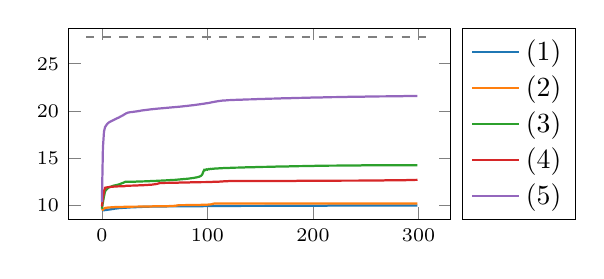
\begin{tikzpicture}

\definecolor{crimson2143940}{RGB}{214,39,40}
\definecolor{darkgray176}{RGB}{176,176,176}
\definecolor{darkorange25512714}{RGB}{255,127,14}
\definecolor{forestgreen4416044}{RGB}{44,160,44}
\definecolor{mediumpurple148103189}{RGB}{148,103,189}
\definecolor{steelblue31119180}{RGB}{31,119,180}

\begin{axis}[compar, legend pos=outer north east]
\addplot [thick, steelblue31119180]
table {%
0 9.43000030517578
1 9.44999980926514
3 9.47000026702881
4 9.48999977111816
5 9.5
6 9.52000045776367
7 9.52999973297119
9 9.56999969482422
10 9.57999992370605
13 9.64000034332275
15 9.65999984741211
16 9.68000030517578
18 9.69999980926514
19 9.69999980926514
22 9.72999954223633
23 9.72999954223633
25 9.75
26 9.75
27 9.76000022888184
28 9.76000022888184
29 9.77000045776367
30 9.77000045776367
31 9.77999973297119
32 9.77999973297119
34 9.80000019073486
35 9.80000019073486
36 9.8100004196167
38 9.8100004196167
39 9.81999969482422
40 9.81999969482422
41 9.82999992370605
44 9.82999992370605
45 9.84000015258789
48 9.84000015258789
49 9.85000038146973
54 9.85000038146973
55 9.85999965667725
61 9.85999965667725
62 9.86999988555908
71 9.86999988555908
72 9.88000011444092
82 9.88000011444092
83 9.89000034332275
96 9.89000034332275
97 9.89999961853027
112 9.89999961853027
113 9.90999984741211
131 9.90999984741211
132 9.92000007629395
154 9.92000007629395
155 9.93000030517578
181 9.93000030517578
182 9.9399995803833
213 9.9399995803833
214 9.94999980926514
251 9.94999980926514
252 9.96000003814697
295 9.96000003814697
296 9.97000026702881
299 9.97000026702881
};
\addlegendentry{$(1)$}
\addplot [thick, darkorange25512714]
table {%
0 9.4399995803833
1 9.52000045776367
2 9.64000034332275
3 9.6899995803833
4 9.72000026702881
5 9.72999954223633
6 9.75
7 9.76000022888184
8 9.76000022888184
10 9.77999973297119
11 9.77999973297119
12 9.78999996185303
14 9.78999996185303
15 9.80000019073486
16 9.80000019073486
17 9.8100004196167
20 9.8100004196167
21 9.81999969482422
24 9.81999969482422
25 9.82999992370605
29 9.82999992370605
30 9.84000015258789
34 9.84000015258789
35 9.85000038146973
40 9.85000038146973
41 9.85999965667725
47 9.85999965667725
48 9.86999988555908
53 9.86999988555908
54 9.88000011444092
59 9.88000011444092
60 9.89000034332275
63 9.89000034332275
64 9.89999961853027
66 9.89999961853027
70 9.9399995803833
72 9.97999954223633
74 10
79 10
80 10.0100002288818
87 10.0100002288818
88 10.0200004577637
93 10.0200004577637
94 10.0299997329712
97 10.0299997329712
98 10.039999961853
99 10.039999961853
103 10.0799999237061
104 10.1000003814697
106 10.1599998474121
107 10.1700000762939
170 10.1700000762939
171 10.1800003051758
299 10.1800003051758
};
\addlegendentry{$(2)$}
\addplot [thick, forestgreen4416044]
table {%
0 9.60999965667725
1 10.289999961853
2 10.9300003051758
3 11.4499998092651
4 11.6199998855591
5 11.710000038147
6 11.8199996948242
7 11.9099998474121
8 11.9399995803833
11 12.0600004196167
12 12.0900001525879
13 12.1099996566772
14 12.1400003433228
15 12.1599998474121
16 12.1899995803833
17 12.2299995422363
18 12.2799997329712
20 12.3599996566772
21 12.4099998474121
22 12.4700002670288
23 12.4799995422363
27 12.4799995422363
28 12.4899997711182
32 12.4899997711182
33 12.5
35 12.5
36 12.5100002288818
38 12.5100002288818
39 12.5200004577637
40 12.5200004577637
41 12.5299997329712
43 12.5299997329712
44 12.539999961853
45 12.539999961853
46 12.5500001907349
47 12.5500001907349
48 12.5600004196167
49 12.5600004196167
50 12.5699996948242
51 12.5699996948242
52 12.5799999237061
53 12.5799999237061
55 12.6000003814697
56 12.6000003814697
57 12.6099996566772
58 12.6099996566772
59 12.6199998855591
60 12.6199998855591
62 12.6400003433228
63 12.6400003433228
65 12.6599998474121
66 12.6599998474121
68 12.6800003051758
69 12.6800003051758
82 12.8100004196167
83 12.8299999237061
84 12.8400001525879
85 12.8599996566772
86 12.8699998855591
90 12.9499998092651
92 13.0100002288818
93 13.0500001907349
94 13.1199998855591
95 13.2299995422363
96 13.5100002288818
97 13.75
98 13.7200002670288
99 13.8000001907349
100 13.7600002288818
101 13.8299999237061
102 13.8100004196167
103 13.8500003814697
104 13.8400001525879
105 13.8699998855591
106 13.8599996566772
107 13.8800001144409
108 13.8800001144409
109 13.8900003433228
110 13.8900003433228
111 13.9099998474121
112 13.9099998474121
113 13.9200000762939
114 13.9200000762939
115 13.9300003051758
117 13.9300003051758
118 13.9399995803833
119 13.9399995803833
120 13.9499998092651
121 13.9499998092651
122 13.960000038147
124 13.960000038147
125 13.9700002670288
126 13.9700002670288
127 13.9799995422363
129 13.9799995422363
130 13.9899997711182
132 13.9899997711182
133 14
135 14
136 14.0100002288818
138 14.0100002288818
139 14.0200004577637
142 14.0200004577637
143 14.0299997329712
145 14.0299997329712
146 14.039999961853
149 14.039999961853
150 14.0500001907349
152 14.0500001907349
153 14.0600004196167
156 14.0600004196167
157 14.0699996948242
160 14.0699996948242
161 14.0799999237061
164 14.0799999237061
165 14.0900001525879
168 14.0900001525879
169 14.1000003814697
172 14.1000003814697
173 14.1099996566772
177 14.1099996566772
178 14.1199998855591
181 14.1199998855591
182 14.1300001144409
186 14.1300001144409
187 14.1400003433228
190 14.1400003433228
191 14.1499996185303
195 14.1499996185303
196 14.1599998474121
201 14.1599998474121
202 14.1700000762939
207 14.1700000762939
208 14.1800003051758
214 14.1800003051758
215 14.1899995803833
222 14.1899995803833
223 14.1999998092651
232 14.1999998092651
233 14.210000038147
245 14.210000038147
246 14.2200002670288
262 14.2200002670288
263 14.2299995422363
281 14.2299995422363
282 14.2399997711182
299 14.2399997711182
};
\addlegendentry{$(3)$}
\addplot [thick, crimson2143940]
table {%
0 9.85000038146973
1 10.7600002288818
2 11.4700002670288
3 11.8400001525879
4 11.8699998855591
5 11.8900003433228
6 11.8999996185303
7 11.9200000762939
12 11.9700002670288
13 11.9700002670288
15 11.9899997711182
16 11.9899997711182
17 12
18 12
19 12.0100002288818
21 12.0100002288818
22 12.0200004577637
23 12.0600004196167
27 12.0600004196167
28 12.0699996948242
29 12.0699996948242
30 12.0799999237061
32 12.0799999237061
33 12.0900001525879
34 12.0900001525879
35 12.1000003814697
36 12.1000003814697
37 12.1099996566772
38 12.1099996566772
39 12.1199998855591
40 12.1199998855591
42 12.1400003433228
43 12.1400003433228
45 12.1599998474121
46 12.1599998474121
48 12.1800003051758
49 12.1999998092651
50 12.210000038147
52 12.25
55 12.3400001525879
56 12.3500003814697
59 12.3500003814697
60 12.3599996566772
63 12.3599996566772
64 12.3699998855591
68 12.3699998855591
69 12.3800001144409
72 12.3800001144409
73 12.3900003433228
76 12.3900003433228
77 12.3999996185303
80 12.3999996185303
81 12.4099998474121
83 12.4099998474121
84 12.4200000762939
88 12.4200000762939
89 12.4300003051758
93 12.4300003051758
94 12.4399995803833
98 12.4399995803833
99 12.4499998092651
101 12.4499998092651
102 12.460000038147
104 12.460000038147
105 12.4700002670288
107 12.4700002670288
108 12.4799995422363
109 12.4799995422363
110 12.4899997711182
111 12.4899997711182
112 12.5
113 12.5
116 12.5299997329712
117 12.5299997329712
118 12.539999961853
119 12.539999961853
120 12.5500001907349
136 12.5500001907349
137 12.5600004196167
160 12.5600004196167
161 12.5699996948242
184 12.5699996948242
185 12.5799999237061
207 12.5799999237061
208 12.5900001525879
226 12.5900001525879
227 12.6000003814697
243 12.6000003814697
244 12.6099996566772
257 12.6099996566772
258 12.6199998855591
267 12.6199998855591
268 12.6300001144409
276 12.6300001144409
277 12.6400003433228
283 12.6400003433228
284 12.6499996185303
288 12.6499996185303
289 12.6599998474121
292 12.6599998474121
293 12.6700000762939
296 12.6700000762939
297 12.6800003051758
298 12.6800003051758
299 12.6899995803833
};
\addlegendentry{$(4)$}
\addplot [thick, mediumpurple148103189]
table {%
0 10.3500003814697
1 16.1200008392334
2 17.7999992370605
3 18.2800006866455
4 18.4400005340576
5 18.6100006103516
6 18.7099990844727
7 18.7999992370605
9 18.9200000762939
10 18.9699993133545
11 19.0300006866455
12 19.0799999237061
13 19.1399993896484
14 19.1900005340576
15 19.25
16 19.2900009155273
17 19.3600006103516
18 19.4099998474121
19 19.4799995422363
20 19.5300006866455
21 19.6100006103516
22 19.6700000762939
23 19.7399997711182
24 19.7800006866455
25 19.8299999237061
26 19.8400001525879
27 19.8700008392334
28 19.8700008392334
29 19.8899993896484
30 19.8999996185303
31 19.9200000762939
32 19.9300003051758
33 19.9500007629395
34 19.9599990844727
35 19.9899997711182
36 20
37 20.0300006866455
38 20.0400009155273
39 20.0599994659424
40 20.0699996948242
41 20.0900001525879
42 20.1000003814697
43 20.1200008392334
44 20.1299991607666
45 20.1499996185303
48 20.1800003051758
49 20.2000007629395
50 20.2000007629395
51 20.2199993133545
76 20.4699993133545
77 20.4899997711182
81 20.5300006866455
82 20.5499992370605
84 20.5699996948242
85 20.5900001525879
87 20.6100006103516
88 20.6299991607666
89 20.6399993896484
90 20.6599998474121
91 20.6700000762939
92 20.6900005340576
93 20.7000007629395
95 20.7399997711182
96 20.75
99 20.8099994659424
100 20.8199996948242
103 20.8799991607666
104 20.9099998474121
111 21.0499992370605
113 21.0699996948242
114 21.0900001525879
116 21.1100006103516
117 21.1100006103516
120 21.1399993896484
121 21.1399993896484
122 21.1499996185303
123 21.1499996185303
124 21.1599998474121
125 21.1599998474121
126 21.1700000762939
127 21.1700000762939
128 21.1800003051758
130 21.1800003051758
131 21.1900005340576
133 21.1900005340576
134 21.2000007629395
135 21.2000007629395
136 21.2099990844727
138 21.2099990844727
139 21.2199993133545
141 21.2199993133545
142 21.2299995422363
143 21.2299995422363
144 21.2399997711182
146 21.2399997711182
147 21.25
149 21.25
150 21.2600002288818
152 21.2600002288818
153 21.2700004577637
154 21.2700004577637
155 21.2800006866455
157 21.2800006866455
158 21.2900009155273
160 21.2900009155273
161 21.2999992370605
163 21.2999992370605
164 21.3099994659424
166 21.3099994659424
167 21.3199996948242
169 21.3199996948242
170 21.3299999237061
172 21.3299999237061
173 21.3400001525879
176 21.3400001525879
177 21.3500003814697
179 21.3500003814697
180 21.3600006103516
182 21.3600006103516
183 21.3700008392334
186 21.3700008392334
187 21.3799991607666
189 21.3799991607666
190 21.3899993896484
193 21.3899993896484
194 21.3999996185303
197 21.3999996185303
198 21.4099998474121
201 21.4099998474121
202 21.4200000762939
205 21.4200000762939
206 21.4300003051758
209 21.4300003051758
210 21.4400005340576
213 21.4400005340576
214 21.4500007629395
217 21.4500007629395
218 21.4599990844727
222 21.4599990844727
223 21.4699993133545
227 21.4699993133545
228 21.4799995422363
232 21.4799995422363
233 21.4899997711182
238 21.4899997711182
239 21.5
243 21.5
244 21.5100002288818
249 21.5100002288818
250 21.5200004577637
255 21.5200004577637
256 21.5300006866455
262 21.5300006866455
263 21.5400009155273
269 21.5400009155273
270 21.5499992370605
277 21.5499992370605
278 21.5599994659424
285 21.5599994659424
286 21.5699996948242
294 21.5699996948242
295 21.5799999237061
299 21.5799999237061
};
\addlegendentry{$(5)$}
\addplot [thick, gray, dashed]
table {%
-14.95 27.8502388000488
313.95 27.8502388000488
};
\end{axis}

\end{tikzpicture}
}
\end{tabular}
	\caption{En première ligne l'initialisation, ensuite la mesure $\bf{y_0}$ de la Target et en desosus le résultat de la LGD après 200 itérations --- sans passe-bas}
	\label{fig:LGD comp_inits g}
\end{figure}

\begin{figure}[H]\centering
	\begin{tabular}{c c c c c c}
Target  &  $(1)$  &  $(2)$  &  $(3)$  &  $(4)$

\\

\multirow{2}{0.3\textwidth}[0.125\textwidth]{\includegraphics[width=0.3\textwidth]{resultats/LGD/inits/inits-target-g.png}}
&
\includegraphics[width=0.15\textwidth]{resultats/LGD/inits/inits_1-init-pas=0.25_filtre=g-0.6.png}
&
\includegraphics[width=0.15\textwidth]{resultats/LGD/inits/inits_2-init-pas=0.25_filtre=g-0.6.png}
&
\includegraphics[width=0.15\textwidth]{resultats/LGD/inits/inits_3-init-pas=0.25_filtre=g-0.6.png}
&
\includegraphics[width=0.15\textwidth]{resultats/LGD/inits/inits_4-init-pas=0.25_filtre=g-0.6.png}

\\


&
\includegraphics[width=0.15\textwidth]{resultats/LGD/inits/inits_1-guess-pas=0.25_filtre=g-0.6.png}
&
\includegraphics[width=0.15\textwidth]{resultats/LGD/inits/inits_2-guess-pas=0.25_filtre=g-0.6.png}
&
\includegraphics[width=0.15\textwidth]{resultats/LGD/inits/inits_3-guess-pas=0.25_filtre=g-0.6.png}
&
\includegraphics[width=0.15\textwidth]{resultats/LGD/inits/inits_4-guess-pas=0.25_filtre=g-0.6.png}

\\ \\



\multicolumn{2}{c}{Loss}  &  \multicolumn{3}{c}{PSNR{\color{white}bbbb}}

\\

\multicolumn{2}{c}{% This file was created with tikzplotlib v0.10.1.
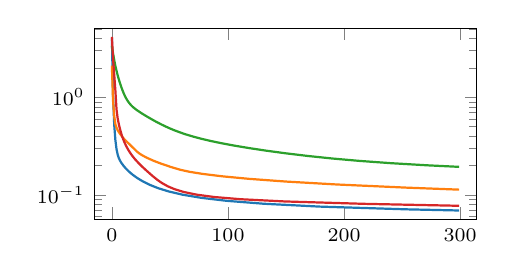
\begin{tikzpicture}

\definecolor{crimson2143940}{RGB}{214,39,40}
\definecolor{darkgray176}{RGB}{176,176,176}
\definecolor{darkorange25512714}{RGB}{255,127,14}
\definecolor{forestgreen4416044}{RGB}{44,160,44}
\definecolor{steelblue31119180}{RGB}{31,119,180}

\begin{axis}[compar,
	ymode=log]
\addplot [thick, steelblue31119180]
table {%
0 4.09705591201782
1 1.0397447347641
2 0.525999307632446
3 0.36544942855835
4 0.294240236282349
5 0.258731842041016
6 0.23837411403656
7 0.2248694896698
8 0.214669942855835
10 0.199013829231262
12 0.18678867816925
15 0.172265887260437
18 0.160792350769043
22 0.148674130439758
27 0.136995673179626
33 0.126390695571899
40 0.117159008979797
49 0.108532667160034
61 0.100532412528992
77 0.0933989286422729
99 0.0870349407196045
131 0.0812307596206665
179 0.0759825706481934
254 0.0712192058563232
299 0.0692975521087646
};
\addplot [thick, darkorange25512714]
table {%
0 2.11676383018494
1 0.9190913438797
2 0.643004417419434
3 0.532035350799561
4 0.487879872322083
5 0.460638880729675
6 0.440029859542847
7 0.422846078872681
9 0.393353462219238
11 0.368957042694092
13 0.349978923797607
22 0.275432348251343
24 0.264232397079468
27 0.25137186050415
31 0.237775444984436
36 0.22367525100708
42 0.210012912750244
51 0.193120121955872
59 0.180989027023315
67 0.172550797462463
78 0.164394378662109
95 0.155235648155212
118 0.146238088607788
150 0.137122750282288
194 0.127958059310913
254 0.118792176246643
299 0.113348960876465
};
\addplot [thick, forestgreen4416044]
table {%
0 3.37779760360718
1 2.81990122795105
2 2.4142701625824
3 2.10492038726807
4 1.86983335018158
5 1.67920529842377
6 1.52351367473602
7 1.3948290348053
8 1.2856605052948
9 1.19226157665253
10 1.11291658878326
11 1.04617238044739
12 0.990375518798828
13 0.94380521774292
14 0.904836654663086
15 0.872018575668335
16 0.844097495079041
17 0.820020079612732
18 0.798925280570984
19 0.780128955841064
21 0.747454047203064
23 0.719166994094849
25 0.693710803985596
28 0.659082055091858
31 0.627551555633545
34 0.598529100418091
38 0.563355803489685
42 0.532020330429077
46 0.504339337348938
50 0.480038523674011
54 0.458757042884827
59 0.435793519020081
64 0.416170716285706
70 0.396113634109497
77 0.376400947570801
85 0.357464551925659
94 0.339470624923706
105 0.320858478546143
118 0.30225658416748
133 0.284092664718628
150 0.266751885414124
169 0.250633358955383
190 0.236100435256958
213 0.223376154899597
240 0.211698055267334
272 0.201091408729553
299 0.194014668464661
};
\addplot [thick, crimson2143940]
table {%
0 4.15872049331665
1 2.48774647712708
2 1.71559143066406
3 1.18148231506348
4 0.74964714050293
5 0.606518745422363
6 0.529028296470642
7 0.472540497779846
8 0.428424477577209
9 0.393683195114136
10 0.365716695785522
11 0.342551231384277
12 0.322939038276672
13 0.306079387664795
14 0.291416645050049
16 0.267123222351074
18 0.247718811035156
20 0.231697797775269
23 0.211907505989075
26 0.195417284965515
30 0.176599979400635
35 0.156593918800354
39 0.143312335014343
43 0.132702112197876
48 0.12282931804657
54 0.114545702934265
62 0.10715639591217
73 0.100697159767151
88 0.0952965021133423
111 0.0903933048248291
149 0.0857839584350586
217 0.0811049938201904
299 0.0774440765380859
};

\end{axis}

\end{tikzpicture}
}
&
\multicolumn{3}{c}{% This file was created with tikzplotlib v0.10.1.
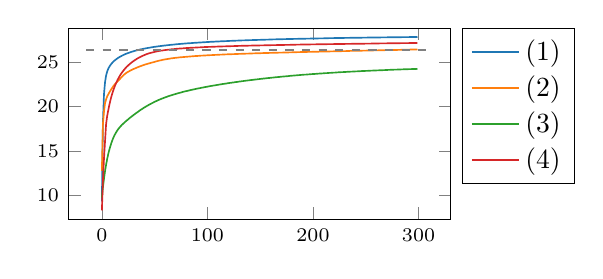
\begin{tikzpicture}

\definecolor{crimson2143940}{RGB}{214,39,40}
\definecolor{darkgray176}{RGB}{176,176,176}
\definecolor{darkorange25512714}{RGB}{255,127,14}
\definecolor{forestgreen4416044}{RGB}{44,160,44}
\definecolor{steelblue31119180}{RGB}{31,119,180}

\begin{axis}[compar, legend pos=outer north east]
\addplot [semithick, steelblue31119180]
table {%
0 9.34000015258789
1 18.2600002288818
2 21.3700008392334
3 22.7199993133545
4 23.4599990844727
5 23.8999996185303
6 24.2099990844727
7 24.4300003051758
8 24.6200008392334
9 24.7700004577637
10 24.9099998474121
11 25.0300006866455
12 25.1399993896484
15 25.4099998474121
16 25.4799995422363
17 25.5599994659424
21 25.7999992370605
24 25.9500007629395
29 26.1499996185303
30 26.1800003051758
31 26.2199993133545
37 26.3999996185303
38 26.4200000762939
39 26.4500007629395
41 26.4899997711182
42 26.5200004577637
50 26.6800003051758
51 26.6900005340576
53 26.7299995422363
54 26.7399997711182
55 26.7600002288818
56 26.7700004577637
57 26.7900009155273
58 26.7999992370605
59 26.8199996948242
61 26.8400001525879
62 26.8600006103516
64 26.8799991607666
65 26.8999996185303
69 26.9400005340576
70 26.9599990844727
82 27.0799999237061
83 27.0799999237061
88 27.1299991607666
89 27.1299991607666
93 27.1700000762939
94 27.1700000762939
96 27.1900005340576
97 27.1900005340576
100 27.2199993133545
101 27.2199993133545
103 27.2399997711182
104 27.2399997711182
105 27.25
106 27.25
108 27.2700004577637
109 27.2700004577637
110 27.2800006866455
111 27.2800006866455
113 27.2999992370605
114 27.2999992370605
115 27.3099994659424
116 27.3099994659424
117 27.3199996948242
118 27.3199996948242
119 27.3299999237061
120 27.3299999237061
121 27.3400001525879
122 27.3400001525879
123 27.3500003814697
124 27.3500003814697
125 27.3600006103516
126 27.3600006103516
127 27.3700008392334
128 27.3700008392334
129 27.3799991607666
130 27.3799991607666
131 27.3899993896484
132 27.3899993896484
133 27.3999996185303
135 27.3999996185303
136 27.4099998474121
137 27.4099998474121
138 27.4200000762939
139 27.4200000762939
140 27.4300003051758
142 27.4300003051758
143 27.4400005340576
144 27.4400005340576
145 27.4500007629395
147 27.4500007629395
148 27.4599990844727
150 27.4599990844727
151 27.4699993133545
153 27.4699993133545
154 27.4799995422363
155 27.4799995422363
156 27.4899997711182
158 27.4899997711182
159 27.5
161 27.5
162 27.5100002288818
164 27.5100002288818
165 27.5200004577637
168 27.5200004577637
169 27.5300006866455
171 27.5300006866455
172 27.5400009155273
174 27.5400009155273
175 27.5499992370605
178 27.5499992370605
179 27.5599994659424
181 27.5599994659424
182 27.5699996948242
185 27.5699996948242
186 27.5799999237061
189 27.5799999237061
190 27.5900001525879
193 27.5900001525879
194 27.6000003814697
197 27.6000003814697
198 27.6100006103516
201 27.6100006103516
202 27.6200008392334
205 27.6200008392334
206 27.6299991607666
210 27.6299991607666
211 27.6399993896484
214 27.6399993896484
215 27.6499996185303
219 27.6499996185303
220 27.6599998474121
224 27.6599998474121
225 27.6700000762939
229 27.6700000762939
230 27.6800003051758
234 27.6800003051758
235 27.6900005340576
240 27.6900005340576
241 27.7000007629395
246 27.7000007629395
247 27.7099990844727
251 27.7099990844727
252 27.7199993133545
257 27.7199993133545
258 27.7299995422363
264 27.7299995422363
265 27.7399997711182
270 27.7399997711182
271 27.75
277 27.75
278 27.7600002288818
284 27.7600002288818
285 27.7700004577637
291 27.7700004577637
292 27.7800006866455
298 27.7800006866455
299 27.7900009155273
};
\addlegendentry{$(1)$}
\addplot [semithick, darkorange25512714]
table {%
0 12.7600002288818
1 18.0300006866455
2 19.4099998474121
3 20.3700008392334
4 20.7800006866455
5 21.1100006103516
7 21.5499992370605
8 21.75
9 21.9400005340576
10 22.1200008392334
11 22.2900009155273
12 22.4400005340576
13 22.5799999237061
16 22.9400005340576
17 23.0699996948242
18 23.1900005340576
19 23.3199996948242
20 23.4400005340576
21 23.5499992370605
22 23.6499996185303
23 23.7399997711182
24 23.8199996948242
25 23.8899993896484
26 23.9500007629395
27 24.0200004577637
28 24.0799999237061
29 24.1299991607666
30 24.1900005340576
36 24.4899997711182
42 24.7299995422363
43 24.7600002288818
44 24.7999992370605
46 24.8600006103516
47 24.8999996185303
50 24.9899997711182
51 25.0300006866455
55 25.1499996185303
56 25.1700000762939
58 25.2299995422363
66 25.3899993896484
67 25.3999996185303
68 25.4200000762939
69 25.4300003051758
70 25.4500007629395
72 25.4699993133545
73 25.4899997711182
89 25.6499996185303
90 25.6499996185303
94 25.6900005340576
95 25.6900005340576
97 25.7099990844727
98 25.7099990844727
100 25.7299995422363
101 25.7299995422363
103 25.75
104 25.75
105 25.7600002288818
106 25.7600002288818
108 25.7800006866455
109 25.7800006866455
110 25.7900009155273
111 25.7900009155273
112 25.7999992370605
113 25.7999992370605
115 25.8199996948242
116 25.8199996948242
117 25.8299999237061
118 25.8299999237061
119 25.8400001525879
120 25.8400001525879
121 25.8500003814697
123 25.8500003814697
124 25.8600006103516
125 25.8600006103516
126 25.8700008392334
127 25.8700008392334
128 25.8799991607666
129 25.8799991607666
130 25.8899993896484
132 25.8899993896484
133 25.8999996185303
134 25.8999996185303
135 25.9099998474121
136 25.9099998474121
137 25.9200000762939
139 25.9200000762939
140 25.9300003051758
142 25.9300003051758
143 25.9400005340576
144 25.9400005340576
145 25.9500007629395
147 25.9500007629395
148 25.9599990844727
150 25.9599990844727
151 25.9699993133545
152 25.9699993133545
153 25.9799995422363
155 25.9799995422363
156 25.9899997711182
158 25.9899997711182
159 26
161 26
162 26.0100002288818
164 26.0100002288818
165 26.0200004577637
167 26.0200004577637
168 26.0300006866455
171 26.0300006866455
172 26.0400009155273
174 26.0400009155273
175 26.0499992370605
177 26.0499992370605
178 26.0599994659424
180 26.0599994659424
181 26.0699996948242
184 26.0699996948242
185 26.0799999237061
187 26.0799999237061
188 26.0900001525879
191 26.0900001525879
192 26.1000003814697
194 26.1000003814697
195 26.1100006103516
198 26.1100006103516
199 26.1200008392334
201 26.1200008392334
202 26.1299991607666
205 26.1299991607666
206 26.1399993896484
208 26.1399993896484
209 26.1499996185303
212 26.1499996185303
213 26.1599998474121
216 26.1599998474121
217 26.1700000762939
219 26.1700000762939
220 26.1800003051758
223 26.1800003051758
224 26.1900005340576
227 26.1900005340576
228 26.2000007629395
231 26.2000007629395
232 26.2099990844727
234 26.2099990844727
235 26.2199993133545
238 26.2199993133545
239 26.2299995422363
242 26.2299995422363
243 26.2399997711182
246 26.2399997711182
247 26.25
250 26.25
251 26.2600002288818
253 26.2600002288818
254 26.2700004577637
257 26.2700004577637
258 26.2800006866455
261 26.2800006866455
262 26.2900009155273
265 26.2900009155273
266 26.2999992370605
268 26.2999992370605
269 26.3099994659424
272 26.3099994659424
273 26.3199996948242
276 26.3199996948242
277 26.3299999237061
280 26.3299999237061
281 26.3400001525879
283 26.3400001525879
284 26.3500003814697
287 26.3500003814697
288 26.3600006103516
291 26.3600006103516
292 26.3700008392334
295 26.3700008392334
296 26.3799991607666
298 26.3799991607666
299 26.3899993896484
};
\addlegendentry{$(2)$}
\addplot [semithick, forestgreen4416044]
table {%
0 9.77999973297119
1 10.9300003051758
2 11.8999996185303
3 12.7399997711182
4 13.460000038147
5 14.0900001525879
6 14.6400003433228
7 15.1099996566772
8 15.5299997329712
9 15.8999996185303
10 16.2299995422363
11 16.5200004577637
12 16.7700004577637
13 16.9899997711182
14 17.1900005340576
15 17.3700008392334
16 17.5300006866455
17 17.6700000762939
19 17.9300003051758
22 18.2600002288818
27 18.7600002288818
32 19.2099990844727
33 19.2900009155273
34 19.3799991607666
35 19.4599990844727
36 19.5499992370605
37 19.6299991607666
38 19.7000007629395
40 19.8600006103516
45 20.2099990844727
51 20.5699996948242
52 20.6200008392334
53 20.6800003051758
57 20.8799991607666
58 20.9200000762939
59 20.9699993133545
61 21.0499992370605
62 21.1000003814697
65 21.2199993133545
66 21.25
68 21.3299999237061
69 21.3600006103516
70 21.3999996185303
71 21.4300003051758
72 21.4699993133545
75 21.5599994659424
76 21.6000003814697
79 21.6900005340576
80 21.7099990844727
84 21.8299999237061
85 21.8500003814697
87 21.9099998474121
88 21.9300003051758
89 21.9599990844727
90 21.9799995422363
91 22.0100002288818
93 22.0499992370605
94 22.0799999237061
96 22.1200008392334
97 22.1499996185303
100 22.2099990844727
101 22.2399997711182
115 22.5200004577637
116 22.5300006866455
121 22.6299991607666
122 22.6399993896484
124 22.6800003051758
125 22.6900005340576
127 22.7299995422363
128 22.7399997711182
130 22.7800006866455
131 22.7900009155273
133 22.8299999237061
134 22.8400001525879
135 22.8600006103516
136 22.8700008392334
137 22.8899993896484
138 22.8999996185303
139 22.9200000762939
140 22.9300003051758
141 22.9500007629395
142 22.9599990844727
143 22.9799995422363
144 22.9899997711182
145 23.0100002288818
147 23.0300006866455
148 23.0499992370605
149 23.0599994659424
150 23.0799999237061
152 23.1000003814697
153 23.1200008392334
155 23.1399993896484
156 23.1599998474121
159 23.1900005340576
160 23.2099990844727
163 23.2399997711182
164 23.2600002288818
168 23.2999992370605
169 23.3199996948242
177 23.3999996185303
178 23.4200000762939
192 23.5599994659424
193 23.5599994659424
201 23.6399993896484
202 23.6399993896484
207 23.6900005340576
208 23.6900005340576
212 23.7299995422363
213 23.7299995422363
216 23.7600002288818
217 23.7600002288818
220 23.7900009155273
221 23.7900009155273
224 23.8199996948242
225 23.8199996948242
227 23.8400001525879
228 23.8400001525879
230 23.8600006103516
231 23.8600006103516
233 23.8799991607666
234 23.8799991607666
236 23.8999996185303
237 23.8999996185303
238 23.9099998474121
239 23.9099998474121
241 23.9300003051758
242 23.9300003051758
243 23.9400005340576
244 23.9400005340576
246 23.9599990844727
247 23.9599990844727
248 23.9699993133545
249 23.9699993133545
250 23.9799995422363
251 23.9799995422363
253 24
254 24
255 24.0100002288818
256 24.0100002288818
257 24.0200004577637
258 24.0200004577637
259 24.0300006866455
260 24.0300006866455
261 24.0400009155273
262 24.0400009155273
263 24.0499992370605
264 24.0499992370605
265 24.0599994659424
266 24.0599994659424
267 24.0699996948242
268 24.0699996948242
269 24.0799999237061
270 24.0799999237061
271 24.0900001525879
272 24.0900001525879
273 24.1000003814697
274 24.1000003814697
275 24.1100006103516
276 24.1100006103516
277 24.1200008392334
279 24.1200008392334
280 24.1299991607666
281 24.1299991607666
282 24.1399993896484
283 24.1399993896484
284 24.1499996185303
285 24.1499996185303
286 24.1599998474121
288 24.1599998474121
289 24.1700000762939
290 24.1700000762939
291 24.1800003051758
293 24.1800003051758
294 24.1900005340576
295 24.1900005340576
296 24.2000007629395
298 24.2000007629395
299 24.2099990844727
};
\addlegendentry{$(3)$}
\addplot [semithick, crimson2143940]
table {%
0 8.32999992370605
1 11.6999998092651
2 14.1499996185303
3 16.1100006103516
4 18.0300006866455
5 18.9099998474121
6 19.5400009155273
7 20.1200008392334
8 20.6399993896484
9 21.1000003814697
10 21.5
11 21.8600006103516
12 22.1900005340576
13 22.4799995422363
14 22.75
15 23
16 23.2199993133545
17 23.4300003051758
18 23.6200008392334
19 23.7900009155273
20 23.9500007629395
21 24.1000003814697
22 24.2399997711182
23 24.3700008392334
24 24.4899997711182
26 24.7099990844727
28 24.9099998474121
29 25
30 25.0799999237061
31 25.1700000762939
32 25.2399997711182
33 25.3199996948242
35 25.4599990844727
38 25.6399993896484
42 25.8400001525879
45 25.9599990844727
51 26.1399993896484
53 26.1800003051758
54 26.2099990844727
56 26.25
57 26.2600002288818
60 26.3199996948242
61 26.3299999237061
62 26.3500003814697
64 26.3700008392334
65 26.3899993896484
69 26.4300003051758
70 26.4500007629395
74 26.4899997711182
75 26.4899997711182
80 26.5400009155273
81 26.5400009155273
84 26.5699996948242
85 26.5699996948242
87 26.5900001525879
88 26.5900001525879
90 26.6100006103516
91 26.6100006103516
92 26.6200008392334
93 26.6200008392334
94 26.6299991607666
95 26.6299991607666
97 26.6499996185303
98 26.6499996185303
99 26.6599998474121
100 26.6599998474121
101 26.6700000762939
103 26.6700000762939
104 26.6800003051758
105 26.6800003051758
106 26.6900005340576
107 26.6900005340576
108 26.7000007629395
109 26.7000007629395
110 26.7099990844727
112 26.7099990844727
113 26.7199993133545
114 26.7199993133545
115 26.7299995422363
117 26.7299995422363
118 26.7399997711182
120 26.7399997711182
121 26.75
122 26.75
123 26.7600002288818
125 26.7600002288818
126 26.7700004577637
128 26.7700004577637
129 26.7800006866455
131 26.7800006866455
132 26.7900009155273
135 26.7900009155273
136 26.7999992370605
138 26.7999992370605
139 26.8099994659424
141 26.8099994659424
142 26.8199996948242
145 26.8199996948242
146 26.8299999237061
149 26.8299999237061
150 26.8400001525879
153 26.8400001525879
154 26.8500003814697
156 26.8500003814697
157 26.8600006103516
160 26.8600006103516
161 26.8700008392334
165 26.8700008392334
166 26.8799991607666
169 26.8799991607666
170 26.8899993896484
173 26.8899993896484
174 26.8999996185303
178 26.8999996185303
179 26.9099998474121
183 26.9099998474121
184 26.9200000762939
187 26.9200000762939
188 26.9300003051758
192 26.9300003051758
193 26.9400005340576
197 26.9400005340576
198 26.9500007629395
202 26.9500007629395
203 26.9599990844727
208 26.9599990844727
209 26.9699993133545
213 26.9699993133545
214 26.9799995422363
219 26.9799995422363
220 26.9899997711182
225 26.9899997711182
226 27
230 27
231 27.0100002288818
236 27.0100002288818
237 27.0200004577637
243 27.0200004577637
244 27.0300006866455
249 27.0300006866455
250 27.0400009155273
255 27.0400009155273
256 27.0499992370605
262 27.0499992370605
263 27.0599994659424
269 27.0599994659424
270 27.0699996948242
275 27.0699996948242
276 27.0799999237061
282 27.0799999237061
283 27.0900001525879
290 27.0900001525879
291 27.1000003814697
297 27.1000003814697
298 27.1100006103516
299 27.1100006103516
};
\addlegendentry{$(4)$}
\addplot [semithick, gray,  dashed]
table {%
-14.95 26.3238544464111
313.95 26.3238544464111
};
\end{axis}

\end{tikzpicture}
}
\end{tabular}
    \caption{En première ligne l'initialisation, ensuite la mesure $\bf{y_0}$ de la Target et en desosus le résultat de la LGD après 200 itérations ---  avec passe-bas gaussien ($\sigma=0.5$)}
	\label{fig:LGD comp_inits g}
\end{figure}
%\\ \\



\subsection{Variation de la taille de l'espace latent}

\begin{figure}[H]\centering
    \includegraphics[width=1\textwidth]{../resultats/LGD/differents latents/lat-s_100_fig.png}
    \caption{$d=100$, sans passe-base}
    \label{fig:LGD comp_size g}
\end{figure}

\begin{figure}[H]\centering
	\includegraphics[width=1\textwidth]{../resultats/LGD/differents latents/lat-g_100_fig.png}
	\caption{$d=100$, avec passe-base}
	\label{fig:LGD comp_size g}
\end{figure}

\begin{figure}[H]\centering
\includegraphics[width=1\textwidth]{../resultats/LGD/differents latents/lat-s_200_fig.png}
\caption{$d=200$, sans passe-base}
\label{fig:LGD comp_size g}
\end{figure}

\begin{figure}[H]\centering
	\includegraphics[width=1\textwidth]{../resultats/LGD/differents latents/lat-g_200_fig.png}
	\caption{$d=200$, avec passe-base}
	\label{fig:LGD comp_size g}
\end{figure}

\begin{figure}[H]\centering
\includegraphics[width=1\textwidth]{../resultats/LGD/differents latents/lat-s_400_fig.png}
\caption{$d=400$, sans passe-base}
\label{fig:LGD comp_size g}
\end{figure}

\begin{figure}[H]\centering
	\includegraphics[width=1\textwidth]{../resultats/LGD/differents latents/lat-g_400_fig.png}
	\caption{$d=400$, avec passe-base}
	\label{fig:LGD comp_size g}
\end{figure}

\begin{figure}[H]\centering
	\includegraphics[width=1\textwidth]{../resultats/LGD/differents latents/lat-g_800_fig.png}
	\caption{$d=800$, avec passe-base}
	\label{fig:LGD comp_size g}
\end{figure}

\begin{figure}[H]\centering
\includegraphics[width=1\textwidth]{../resultats/LGD/differents latents/lat-s_800_fig.png}
\caption{$d=800$, sans passe-base}
\label{fig:LGD comp_size g}
\end{figure}
\`A noter que sur la loss de la figure \figref{fig:LGD comp_size g} lees algorithmes stagnent ce qui sous entend que l'on se trouve dans des vallées (ou des crêtes). Problème qui peut être évité en ajoutant de l'inertie à la descente avec des méthodes type heavy-ball ou Nesterof. 





\newpage



\section{Comparaison avec la descente de gradient projetée}\label{sec:comparPGD}

\subsection{Le principe et les résultats}\label{sec:PGD}
\quad 

La descente de gradient projeté par auto-encodeur était sensé faire office d'algorithme de contrôle. Comme son nom l'indique, la descente de gradient projeté (PGD) consiste en une descente de gradient classique à cela près qu'à itération, le vecteur obtenu est projeté par une fonction$f$ (voir \figref{fig:pcode PGD} ci-contre). 

\begin{wrapfigure}[17]{r}{0.38\textwidth}
    \fbox{\begin{minipage}{18em}
\vspace{0.3cm}
\begin{algorithmic}[0]
    \State $x_0$ : initialisation
    \State $x$ : image à reconstruire
    \State $\rho$ : pas de descente
    \State $N$ : nombre d'itération
    \State $y\ \ll\ A(x)$
    \State
    \For{$n\in \llbracket1,N-1\rrbracket$}
        \State $\nabla F(x_n)\ \ll\ ^tA\big(Ax_n-y_0\big)$
        \State $\ \ x_{n+1}\quad  \ll\ p\big(x_n\ - \rho \nabla F(x_n)\big)$
        \EndFor
    \State
    \Return $(x_n)_{0\leq n\leq N}$
\end{algorithmic}
\vspace{0.2cm}
\end{minipage}}
    \caption{Algorithme de PGD}
    \label{fig:pcode PGD}
\end{wrapfigure}
\noindent Dans notre cas, $f$ est un auto-encoder dont on notera $f_E$ et $f_D$ les parties encodage et décodage respectivement, de sorte que :
\[f = f_D\circ f_E\]{\color{white}l}
\\
Cette méthode est tirée de l'article \cite{peng_solving_2019} de P. Peng, S. Jalali and X. Yuan, et leurs résultats étaient satisfaisant. Pourtant comme on va le voir dans la section \ref{sec:res PGD} plus bas, nous n'avons pas réussi à les reproduire.
Cela étant dit, nous allons malgré tout détailler l'algorithme et essayer de comprendre les résultats obtenus.
\\
Ce rapport étant surtout porté sur la descente de gradient depuis l'espace lattent de $f$, on ne détaillera pas les arguments mathématiques qui supportent cette méthode mais on peut tout de même essayer de se convaincre de l'intérêt de la PGD.\\
Comme expliqué plus haut, le problème est convexe ce qui assure la convergence de la descente de gradient. La difficulté étant de tomber sur le bon argmin. C'est là que composer par $f$ peut aider à diriger la descente vers le ``bon'' minimum.


\begin{itemize}
	\item Converge beaucoup plus vite
	\item Sensible à l'excès d'itérations (sûrement parce que $f$ n'est pas une vrai identité, c'est un problème classique)
	\item Très sensible au pas image-wise
	\item Robuste à l'initialisation
\end{itemize}
\\ \\



\subsection{Comparaison avec la LGD}\label{sec:res PGD}
\begin{figure}[H]\centering
    %\begin{tabular}{c c c}

Image cible $\bf{x_0}$  &  Image reconstruite par PGD  &  Évolution de $F$

\\

\includegraphics[width=0.25\textwidth]{resultats (legacy)/PGD/seed21-target-pas=1e-10_filtre=g-0.6.png}
&
\includegraphics[width=0.25\textwidth]{resultats (legacy)/PGD/seed21-guess-pas=1e-10_filtre=s-None.png}&
% This file was created with tikzplotlib v0.10.1.
\begin{tikzpicture}

\definecolor{darkgray176}{RGB}{176,176,176}

\begin{axis}[
height=\figheight,
tick align=outside,
tick pos=left,
width=\figwidth,
x grid style={darkgray176},
xmin=-14.95, xmax=313.95,
xtick style={color=black},
y grid style={darkgray176},
ymin=-0.27700514793396, ymax=5.81710810661316,
ytick style={color=black}
]
\addplot [semithick, blue]
table {%
0 0
1 3.99918556213379
2 4.4326753616333
3 4.64342212677002
4 4.81190347671509
5 4.91778469085693
6 4.94641876220703
7 5.00477170944214
8 5.08310174942017
9 5.19564056396484
10 5.28801679611206
11 5.33263826370239
12 5.33070850372314
13 5.27263307571411
14 5.23092842102051
15 5.23794794082642
16 5.26272058486938
17 5.29059505462646
19 5.31402111053467
20 5.33875274658203
21 5.34798526763916
22 5.35215950012207
23 5.38403081893921
24 5.4258508682251
25 5.44844102859497
27 5.50888061523438
28 5.52512788772583
29 5.53270483016968
31 5.53947687149048
32 5.5401029586792
33 5.53452062606812
34 5.5092601776123
35 5.46018075942993
36 5.37410974502563
37 5.3332576751709
38 5.29860496520996
40 5.30271196365356
42 5.30756855010986
44 5.30643606185913
46 5.29865407943726
48 5.28588056564331
56 5.21698045730591
57 5.21158313751221
58 5.20865535736084
59 5.209068775177
60 5.21390819549561
63 5.24272871017456
64 5.24536895751953
65 5.24342823028564
70 5.22004127502441
72 5.21739292144775
74 5.21886348724365
78 5.23052501678467
79 5.22513961791992
80 5.212806224823
81 5.19291114807129
82 5.16722202301025
83 5.14391422271729
84 5.13343667984009
85 5.13356256484985
87 5.1406569480896
88 5.15007829666138
89 5.17058277130127
90 5.19438791275024
91 5.21577215194702
92 5.24896907806396
93 5.27364110946655
94 5.28173780441284
95 5.27473545074463
96 5.27097177505493
97 5.29448747634888
98 5.30808019638062
99 5.30341196060181
100 5.2866268157959
102 5.24024200439453
104 5.19818449020386
105 5.18349599838257
106 5.17607545852661
108 5.16804647445679
109 5.15885734558105
110 5.13583183288574
111 5.10354614257812
112 5.08050298690796
113 5.07250070571899
115 5.07139158248901
117 5.07495975494385
118 5.07892990112305
119 5.08528852462769
120 5.09469795227051
121 5.10748672485352
122 5.1234245300293
125 5.180419921875
126 5.18454790115356
128 5.16531324386597
129 5.15809011459351
130 5.15367698669434
131 5.15327548980713
132 5.15048885345459
133 5.12789678573608
134 5.08534717559814
135 5.06577205657959
136 5.05729579925537
137 5.04308748245239
139 4.99286603927612
141 4.95676374435425
142 4.94296407699585
143 4.93803787231445
146 4.94216871261597
149 4.93214082717896
152 4.9313497543335
159 4.93366098403931
162 4.93031597137451
163 4.92670583724976
164 4.92089653015137
165 4.91259574890137
166 4.90145063400269
167 4.88670587539673
168 4.86730337142944
169 4.84241771697998
170 4.81184577941895
171 4.77796459197998
172 4.74916410446167
173 4.73338079452515
174 4.72774791717529
176 4.72406816482544
177 4.72806692123413
178 4.73987293243408
179 4.74806642532349
180 4.75052118301392
182 4.74916124343872
185 4.7413182258606
190 4.72596502304077
192 4.72232913970947
194 4.72235822677612
197 4.7260684967041
198 4.72343730926514
199 4.71675395965576
200 4.70512437820435
201 4.68725967407227
202 4.66130685806274
203 4.62429666519165
204 4.57392072677612
205 4.51885461807251
206 4.47372627258301
207 4.4455943107605
208 4.4383864402771
209 4.44177770614624
211 4.456467628479
213 4.47890567779541
216 4.51510190963745
218 4.53515195846558
221 4.56325340270996
223 4.58339595794678
225 4.59782600402832
227 4.60461473464966
230 4.60779857635498
238 4.60866546630859
299 4.60859251022339
};
\end{axis}

\end{tikzpicture}


\\ \\

Image cible compressée $A(\bf{x_0})$  &  Initialisation de la PGD  & Évolution de PSNR

\\

\includegraphics[width=0.25\textwidth]{resultats (legacy)/PGD/seed21-comptarg-pas=1e-10_filtre=s-None.png}
&
\includegraphics[width=0.25\textwidth]{resultats (legacy)/PGD/seed21-init-pas=1e-10_filtre=s-None.png}
&
% This file was created with tikzplotlib v0.10.1.
\begin{tikzpicture}

\definecolor{darkgray176}{RGB}{176,176,176}
\definecolor{orange}{RGB}{255,165,0}

\begin{axis}[
height=\figheight,
tick align=outside,
tick pos=left,
width=\figwidth,
x grid style={darkgray176},
xmin=-14.95, xmax=313.95,
xtick style={color=black},
y grid style={darkgray176},
ymin=7.90699973106384, ymax=10.6129997730255,
ytick style={color=black}
]
\addplot [semithick, orange]
table {%
0 10.1300001144409
1 10.4899997711182
2 9.81999969482422
3 9.35999965667725
4 9.1899995803833
5 9.06999969482422
6 9.01000022888184
7 8.89999961853027
8 8.76000022888184
10 8.57999992370605
11 8.47999954223633
12 8.44999980926514
14 8.44999980926514
15 8.4399995803833
16 8.40999984741211
17 8.39000034332275
19 8.40999984741211
20 8.36999988555908
22 8.21000003814697
23 8.14000034332275
24 8.09000015258789
27 8.02999973297119
33 8.02999973297119
34 8.05000019073486
35 8.11999988555908
36 8.22999954223633
37 8.3100004196167
38 8.34000015258789
39 8.35999965667725
41 8.35999965667725
42 8.35000038146973
43 8.32999992370605
45 8.32999992370605
50 8.38000011444092
51 8.39999961853027
52 8.40999984741211
53 8.43000030517578
54 8.4399995803833
55 8.46000003814697
56 8.46000003814697
57 8.47000026702881
60 8.47000026702881
61 8.46000003814697
62 8.46000003814697
65 8.43000030517578
66 8.43000030517578
67 8.42000007629395
68 8.42000007629395
69 8.43000030517578
70 8.43000030517578
72 8.44999980926514
73 8.44999980926514
75 8.47000026702881
76 8.47000026702881
80 8.51000022888184
81 8.52999973297119
82 8.53999996185303
84 8.53999996185303
85 8.55000019073486
87 8.55000019073486
88 8.53999996185303
91 8.44999980926514
93 8.40999984741211
96 8.40999984741211
97 8.39000034332275
100 8.35999965667725
101 8.36999988555908
102 8.39000034332275
103 8.39999961853027
104 8.39999961853027
105 8.40999984741211
106 8.40999984741211
109 8.47000026702881
113 8.59000015258789
115 8.60999965667725
117 8.60999965667725
118 8.60000038146973
119 8.60000038146973
120 8.59000015258789
121 8.56999969482422
122 8.5600004196167
123 8.53999996185303
125 8.46000003814697
126 8.46000003814697
130 8.61999988555908
131 8.64999961853027
132 8.6899995803833
134 8.78999996185303
136 8.86999988555908
137 8.89999961853027
138 8.9399995803833
141 9.02999973297119
143 9.02999973297119
148 8.97999954223633
149 8.97999954223633
150 8.97000026702881
151 8.97000026702881
152 8.96000003814697
153 8.96000003814697
154 8.94999980926514
156 8.94999980926514
157 8.9399995803833
162 8.9399995803833
165 8.97000026702881
168 9.02999973297119
171 9.11999988555908
176 9.22000026702881
177 9.22999954223633
179 9.22999954223633
181 9.25
182 9.25
183 9.26000022888184
184 9.26000022888184
185 9.27000045776367
187 9.27000045776367
188 9.27999973297119
192 9.27999973297119
194 9.26000022888184
197 9.26000022888184
199 9.27999973297119
201 9.31999969482422
204 9.40999984741211
206 9.48999977111816
207 9.52000045776367
208 9.53999996185303
210 9.5600004196167
213 9.52999973297119
214 9.51000022888184
218 9.47000026702881
224 9.47000026702881
225 9.46000003814697
228 9.46000003814697
229 9.44999980926514
299 9.44999980926514
};
\end{axis}

\end{tikzpicture}


\end{tabular}
    \caption{Résultat de la PGD avec un pas de descente $\rho=10^{-10}$, sans passe-bas}
\end{figure}

\begin{figure}[H]\centering
    %\begin{tabular}{c c c}

Image cible $\bf{x_0}$  &  Image reconstruite par PGD  &  Évolution de $F$

\\

\includegraphics[width=0.25\textwidth]{resultats (legacy)/PGD/seed21-target-pas=1e-10_filtre=g-0.6.png}
&
\includegraphics[width=0.25\textwidth]{resultats (legacy)/PGD/seed21-guess-pas=1e-10_filtre=g-0.6.png}&
% This file was created with tikzplotlib v0.10.1.
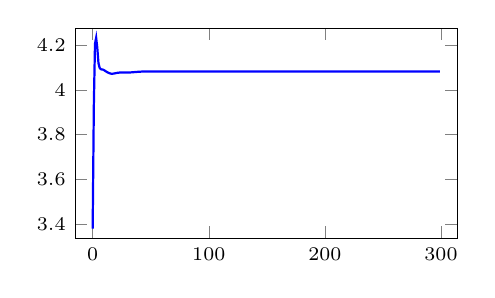
\begin{tikzpicture}

\definecolor{darkgray176}{RGB}{176,176,176}

\begin{axis}[standard]
\addplot [thick, blue]
table {%
0 3.38101553916931
1 3.92825508117676
2 4.2053689956665
3 4.2320728302002
4 4.1864185333252
5 4.11872434616089
6 4.09811353683472
7 4.09209442138672
8 4.09062051773071
9 4.08995199203491
10 4.08711194992065
12 4.08036422729492
13 4.07745313644409
14 4.07500076293945
15 4.07309627532959
16 4.07194423675537
17 4.07178068161011
18 4.07246017456055
21 4.07559776306152
23 4.07689714431763
25 4.07709217071533
29 4.07682323455811
32 4.07738208770752
36 4.07902431488037
40 4.08074569702148
43 4.08150815963745
48 4.08195686340332
61 4.08205604553223
299 4.08205652236938
};
\end{axis}

\end{tikzpicture}


\\ \\

Image cible compressée $A(\bf{x_0})$  &  Initialisation de la PGD  & Évolution de PSNR

\\

\includegraphics[width=0.25\textwidth]{resultats (legacy)/PGD/seed21-comptarg-pas=1e-10_filtre=g-0.6.png}
&
\includegraphics[width=0.25\textwidth]{resultats (legacy)/PGD/seed21-init-pas=1e-10_filtre=g-0.6.png}
&
% This file was created with tikzplotlib v0.10.1.
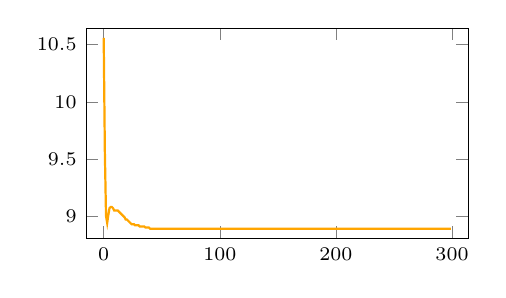
\begin{tikzpicture}

\definecolor{darkgray176}{RGB}{176,176,176}
\definecolor{orange}{RGB}{255,165,0}

\begin{axis}[standard]
\addplot [thick, orange]
table {%
0 10.5600004196167
1 9.5600004196167
2 9
3 8.9399995803833
4 9.01000022888184
5 9.06999969482422
6 9.07999992370605
7 9.07999992370605
8 9.06999969482422
9 9.05000019073486
12 9.05000019073486
18 8.98999977111816
19 8.97000026702881
20 8.97000026702881
24 8.93000030517578
26 8.93000030517578
27 8.92000007629395
30 8.92000007629395
31 8.90999984741211
35 8.90999984741211
36 8.89999961853027
39 8.89999961853027
40 8.89000034332275
299 8.89000034332275
};
\end{axis}

\end{tikzpicture}


\end{tabular}
    \caption{Résultat de la PGD avec un pas de descente $\rho=10^{-10}$, passe-bas gaussien ($\sigma=0.6$)}
\end{figure}

\begin{figure}[H]\centering
    %\begin{tabular}{c c c c c c c}
Target  &  $(1)$  &  $(2)$  &  $(3)$  &  $(4)$  &  $(5)$  &  $(6)$

\\

\includegraphics[width=0.12\textwidth]{resultats (legacy)/PGD/comp-pas-s1-target-pas=0.01_filtre=s-None.png}
&
\includegraphics[width=0.12\textwidth]{resultats (legacy)/PGD/comp-pas-s1_1-guess-pas=1.1_filtre=s-None.png}
&
\includegraphics[width=0.12\textwidth]{resultats (legacy)/PGD/comp-pas-s1_2-guess-pas=0.9_filtre=s-None.png}
&
\includegraphics[width=0.12\textwidth]{resultats (legacy)/PGD/comp-pas-s1_3-guess-pas=0.7_filtre=s-None.png}
&
\includegraphics[width=0.12\textwidth]{resultats (legacy)/PGD/comp-pas-s1_4-guess-pas=0.5_filtre=s-None.png}
&
\includegraphics[width=0.12\textwidth]{resultats (legacy)/PGD/comp-pas-s1_5-guess-pas=0.1_filtre=s-None.png}
&
\includegraphics[width=0.12\textwidth]{resultats (legacy)/PGD/comp-pas-s1_6-guess-pas=0.01_filtre=s-None.png}

\\
&  $\rho=1.1$  &  $\rho=0.9$  &  $\rho=0.7$  &  $\rho=0.5$  &  $\rho=0.1$  &  $\rho=0.01$

\\ \\


\multicolumn{3}{c}{\quad Évolution des loss}
&
\multicolumn{3}{c}{\qquad\qquad Évolution des PSNR}

\\

\multicolumn{3}{c}{% This file was created with tikzplotlib v0.10.1.
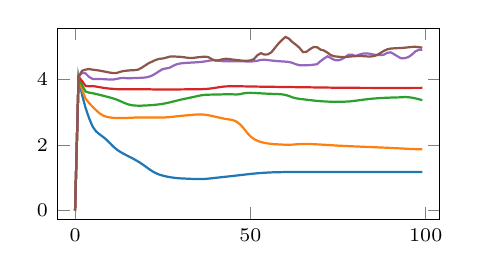
\begin{tikzpicture}

\definecolor{crimson2143940}{RGB}{214,39,40}
\definecolor{darkgray176}{RGB}{176,176,176}
\definecolor{darkorange25512714}{RGB}{255,127,14}
\definecolor{forestgreen4416044}{RGB}{44,160,44}
\definecolor{mediumpurple148103189}{RGB}{148,103,189}
\definecolor{sienna1408675}{RGB}{140,86,75}
\definecolor{steelblue31119180}{RGB}{31,119,180}

\begin{axis}[compar]
\addplot [thick, steelblue31119180]
table {%
0 0
1 4.07896375656128
2 3.52517080307007
3 3.12815141677856
4 2.81518316268921
5 2.56268668174744
6 2.41218519210815
7 2.32254910469055
8 2.24398493766785
9 2.1550874710083
10 2.04974150657654
11 1.94149577617645
12 1.85119020938873
13 1.78053987026215
14 1.72163999080658
16 1.61274838447571
17 1.55523943901062
18 1.49298596382141
19 1.4247362613678
20 1.35008704662323
21 1.27169048786163
22 1.19849848747253
23 1.14036464691162
24 1.09690809249878
25 1.06362283229828
26 1.03781700134277
27 1.01737356185913
28 1.00106072425842
29 0.98879337310791
30 0.980517625808716
33 0.965440154075623
35 0.957900524139404
36 0.957945704460144
37 0.962774991989136
38 0.972147226333618
46 1.06584620475769
50 1.11546194553375
52 1.1362316608429
54 1.15210509300232
56 1.16279006004333
58 1.16916263103485
61 1.1736353635788
66 1.17550802230835
90 1.17538797855377
99 1.17537343502045
};
\addplot [thick, darkorange25512714]
table {%
0 0
1 4.07896375656128
2 3.68217897415161
3 3.41303467750549
4 3.27746367454529
5 3.16378164291382
6 3.05855870246887
7 2.96412682533264
8 2.89624261856079
9 2.85797500610352
10 2.83769059181213
11 2.82628059387207
12 2.82035517692566
13 2.81888937950134
14 2.82101798057556
18 2.83915281295776
20 2.839919090271
24 2.83509492874146
25 2.8367612361908
26 2.84170770645142
27 2.85064959526062
31 2.89562010765076
34 2.92370295524597
35 2.93018984794617
36 2.93084073066711
37 2.92324113845825
38 2.90725541114807
39 2.88498115539551
42 2.81203198432922
43 2.79147887229919
44 2.77665281295776
45 2.7579562664032
46 2.71232795715332
47 2.63271260261536
48 2.51651525497437
49 2.37964010238647
50 2.26284599304199
51 2.18112254142761
52 2.12654852867126
53 2.08971452713013
54 2.06392884254456
55 2.04536175727844
56 2.03200602531433
57 2.02255630493164
59 2.01067805290222
60 2.00684094429016
61 2.00561332702637
62 2.00979232788086
64 2.02727031707764
65 2.03128576278687
66 2.0311872959137
68 2.02385687828064
71 2.00536942481995
75 1.9788613319397
78 1.96282684803009
83 1.94115149974823
89 1.91430306434631
93 1.89214110374451
96 1.87565422058105
99 1.86520540714264
};
\addplot [thick, forestgreen4416044]
table {%
0 0
1 4.07896375656128
2 3.8205451965332
3 3.62880373001099
4 3.59577369689941
5 3.57894825935364
7 3.52864384651184
9 3.47441124916077
10 3.44589066505432
11 3.41447138786316
12 3.37740063667297
13 3.3326997756958
14 3.28390336036682
15 3.2418737411499
16 3.21481728553772
17 3.20173120498657
18 3.19775176048279
19 3.19886231422424
21 3.2087984085083
22 3.2165834903717
23 3.22645115852356
24 3.23891043663025
25 3.25468277931213
26 3.27456378936768
27 3.29879713058472
30 3.37813758850098
36 3.51523613929749
37 3.52785992622375
38 3.53350329399109
42 3.542884349823
43 3.54671359062195
44 3.54803013801575
46 3.53936624526978
47 3.54797315597534
48 3.57345414161682
49 3.5877788066864
50 3.58951210975647
51 3.58553290367126
55 3.56243348121643
58 3.55092120170593
59 3.54289412498474
60 3.5255331993103
61 3.49262976646423
62 3.45118856430054
63 3.42291903495789
64 3.40627121925354
68 3.35461449623108
70 3.33442378044128
72 3.32210063934326
74 3.31670355796814
76 3.31729507446289
77 3.32043409347534
78 3.32643532752991
79 3.3359112739563
81 3.36291480064392
83 3.39171957969666
85 3.41468930244446
87 3.43023324012756
89 3.44056844711304
91 3.44824767112732
93 3.45331287384033
94 3.46086668968201
95 3.45691871643066
96 3.44251346588135
97 3.42187762260437
98 3.39602041244507
99 3.36537027359009
};
\addplot [thick, crimson2143940]
table {%
0 0
1 4.07896375656128
2 3.94823622703552
3 3.80108308792114
4 3.78965187072754
5 3.79547238349915
6 3.78107476234436
8 3.7436625957489
9 3.72878503799438
10 3.71715617179871
11 3.70839047431946
12 3.70217561721802
13 3.69829487800598
15 3.69651627540588
19 3.70093441009521
21 3.69738125801086
24 3.69032216072083
26 3.69020771980286
36 3.70123338699341
37 3.70583987236023
38 3.71418929100037
39 3.72724795341492
42 3.77587366104126
43 3.78566789627075
44 3.79075264930725
45 3.79218196868896
47 3.78928422927856
52 3.77963805198669
74 3.74674415588379
82 3.74110007286072
91 3.73915147781372
98 3.74113392829895
99 3.74187564849854
};
\addplot [thick, mediumpurple148103189]
table {%
0 0
1 4.07896375656128
2 4.20143127441406
3 4.18282270431519
4 4.07413816452026
5 4.01319360733032
6 4.0098295211792
8 4.00828313827515
10 3.9943208694458
11 3.99805307388306
13 4.03817749023438
14 4.04082536697388
15 4.03497409820557
16 4.03643465042114
19 4.04919767379761
20 4.05767297744751
21 4.07760524749756
22 4.11900758743286
23 4.18120098114014
24 4.25132083892822
25 4.3161096572876
26 4.33346223831177
27 4.35759210586548
28 4.41550207138062
29 4.46173143386841
30 4.48590850830078
31 4.49872064590454
33 4.51173448562622
35 4.52376794815063
36 4.53285932540894
37 4.54655408859253
38 4.56601190567017
39 4.58160257339478
40 4.58052206039429
42 4.55558919906616
43 4.55141973495483
45 4.55555009841919
46 4.55513620376587
50 4.5451512336731
51 4.55182218551636
52 4.56834697723389
53 4.59388399124146
54 4.60153150558472
57 4.56292104721069
59 4.54803514480591
60 4.54122066497803
61 4.53067779541016
62 4.50368785858154
63 4.4599347114563
64 4.43334245681763
65 4.42784452438354
66 4.43072175979614
67 4.43723678588867
68 4.44729900360107
69 4.46444177627563
70 4.55684423446655
71 4.63702630996704
72 4.70514965057373
74 4.59016847610474
75 4.57998275756836
76 4.61408805847168
77 4.67671489715576
78 4.75459003448486
79 4.75405120849609
80 4.71129560470581
81 4.75442266464233
82 4.78543329238892
83 4.79236507415771
84 4.78348731994629
85 4.75929403305054
86 4.74150371551514
87 4.74146127700806
88 4.75127363204956
89 4.80999851226807
90 4.82527351379395
91 4.76644897460938
92 4.69950532913208
93 4.6431303024292
94 4.64853620529175
95 4.67958164215088
96 4.75133943557739
97 4.85158443450928
98 4.90142774581909
99 4.90428638458252
};
\addplot [thick, sienna1408675]
table {%
0 0
1 4.07896375656128
2 4.26257085800171
3 4.29840040206909
4 4.31559228897095
5 4.29680633544922
6 4.28421878814697
7 4.26799869537354
10 4.20488739013672
11 4.19218683242798
12 4.20002508163452
13 4.2350492477417
14 4.2576265335083
15 4.26918935775757
16 4.27773427963257
17 4.28240823745728
18 4.29785299301147
19 4.35661697387695
21 4.49404048919678
23 4.59406995773315
24 4.62606239318848
25 4.63771677017212
26 4.66309595108032
27 4.6948127746582
28 4.69933652877808
30 4.68756246566772
31 4.67648220062256
32 4.660475730896
33 4.64902544021606
34 4.65869140625
35 4.67483520507812
37 4.69446039199829
38 4.67967176437378
39 4.61586284637451
40 4.57644414901733
41 4.58235645294189
42 4.61419677734375
43 4.62959957122803
44 4.61973333358765
45 4.60397577285767
48 4.56872510910034
49 4.5660080909729
50 4.57988357543945
51 4.61799669265747
52 4.73879051208496
53 4.79972267150879
54 4.75632619857788
55 4.76513814926147
56 4.82943058013916
58 5.09398937225342
59 5.20115375518799
60 5.29610347747803
61 5.24005365371704
62 5.13516235351562
63 5.0555944442749
64 4.96172857284546
65 4.83070421218872
66 4.84230327606201
67 4.92264270782471
68 4.98552894592285
69 4.98272562026978
70 4.90815019607544
71 4.87900400161743
72 4.81329298019409
73 4.73470258712769
74 4.70453357696533
75 4.69143533706665
76 4.68353652954102
77 4.68474006652832
78 4.69263648986816
80 4.71166610717773
81 4.714515209198
82 4.70982027053833
84 4.69606494903564
85 4.70591306686401
86 4.73970317840576
87 4.79891109466553
88 4.86688661575317
89 4.91673183441162
90 4.93967008590698
91 4.94825172424316
93 4.95826292037964
94 4.96681976318359
96 4.99044322967529
97 4.9943642616272
98 4.98428583145142
99 4.96689653396606
};
\end{axis}

\end{tikzpicture}
}
&
\multicolumn{4}{c}{% This file was created with tikzplotlib v0.10.1.
\begin{tikzpicture}

\definecolor{crimson2143940}{RGB}{214,39,40}
\definecolor{darkgray176}{RGB}{176,176,176}
\definecolor{darkorange25512714}{RGB}{255,127,14}
\definecolor{forestgreen4416044}{RGB}{44,160,44}
\definecolor{mediumpurple148103189}{RGB}{148,103,189}
\definecolor{sienna1408675}{RGB}{140,86,75}
\definecolor{steelblue31119180}{RGB}{31,119,180}

\begin{axis}[
height=\figheight,
tick align=outside,
tick pos=left,
width=\figwidth,
x grid style={darkgray176},
xmin=-4.95, xmax=103.95,
xtick style={color=black},
y grid style={darkgray176},
ymin=8.03750014305115, ymax=21.0724995136261,
ytick style={color=black}
]
\addplot [semithick, steelblue31119180]
table {%
0 11.1400003433228
1 12.1999998092651
2 13.460000038147
3 14.3699998855591
4 14.8999996185303
5 15.2399997711182
6 15.5
7 15.7299995422363
8 15.9499998092651
9 16.1599998474121
10 16.3600006103516
11 16.5200004577637
12 16.6499996185303
13 16.7600002288818
14 16.8899993896484
15 17.0300006866455
16 17.1900005340576
17 17.3899993896484
18 17.6399993896484
19 17.9500007629395
20 18.3400001525879
21 18.7600002288818
22 19.1599998474121
23 19.4799995422363
24 19.75
25 19.9699993133545
26 20.1399993896484
27 20.2700004577637
28 20.3400001525879
29 20.3799991607666
31 20.4400005340576
33 20.4799995422363
34 20.4699993133545
35 20.4099998474121
37 20.2299995422363
38 20.1599998474121
39 20.1200008392334
40 20.0900001525879
42 20.0100002288818
43 19.9599990844727
44 19.8999996185303
45 19.8299999237061
46 19.75
50 19.3899993896484
52 19.2299995422363
54 19.1100006103516
55 19.0599994659424
56 19.0200004577637
58 18.9599990844727
59 18.9400005340576
63 18.8999996185303
64 18.8999996185303
65 18.8899993896484
69 18.8899993896484
70 18.8799991607666
98 18.8799991607666
99 18.3299999237061
};
\addplot [semithick, darkorange25512714]
table {%
0 11.1400003433228
1 12.1999998092651
2 13.1000003814697
3 13.7200002670288
4 14.0100002288818
5 14.1700000762939
7 14.3900003433228
8 14.4799995422363
9 14.5299997329712
10 14.5600004196167
11 14.5600004196167
12 14.5500001907349
13 14.5200004577637
15 14.4399995803833
18 14.3500003814697
20 14.3100004196167
21 14.2799997329712
23 14.1999998092651
24 14.1700000762939
26 14.0900001525879
28 14.0299997329712
29 14.0100002288818
32 13.9799995422363
34 13.9799995422363
35 13.9899997711182
36 14.0100002288818
37 14.0500001907349
38 14.1099996566772
39 14.1800003051758
40 14.2600002288818
43 14.5299997329712
44 14.6300001144409
45 14.7700004577637
46 14.9700002670288
48 15.4700002670288
49 15.6899995803833
50 15.8699998855591
51 16.0200004577637
52 16.1399993896484
53 16.2199993133545
54 16.2800006866455
55 16.3199996948242
56 16.3400001525879
57 16.3500003814697
58 16.3400001525879
59 16.3199996948242
60 16.2800006866455
61 16.2199993133545
62 16.1499996185303
63 16.1100006103516
64 16.1000003814697
65 16.1000003814697
68 16.1299991607666
69 16.1499996185303
76 16.2199993133545
77 16.2199993133545
78 16.2299995422363
84 16.2299995422363
85 16.2199993133545
87 16.2199993133545
88 16.2099990844727
90 16.2099990844727
95 16.1599998474121
96 16.1399993896484
98 16.1200008392334
99 15.3900003433228
};
\addplot [semithick, forestgreen4416044]
table {%
0 11.1400003433228
1 12.0799999237061
2 12.6700000762939
3 13.0699996948242
4 13.210000038147
8 13.3699998855591
11 13.5200004577637
13 13.6400003433228
14 13.6899995803833
15 13.7299995422363
16 13.75
17 13.75
18 13.7399997711182
22 13.6599998474121
23 13.6300001144409
24 13.6099996566772
25 13.5699996948242
26 13.5200004577637
29 13.3400001525879
30 13.3000001907349
31 13.25
32 13.210000038147
34 13.1099996566772
35 13.0699996948242
36 13.039999961853
37 13.0200004577637
39 13
40 12.9700002670288
41 12.9499998092651
42 12.9099998474121
43 12.8800001144409
44 12.8599996566772
45 12.8599996566772
46 12.8699998855591
47 12.8699998855591
49 12.8500003814697
51 12.8699998855591
52 12.8900003433228
53 12.9200000762939
57 13
59 13.0600004196167
61 13.1400003433228
62 13.1300001144409
63 13.0799999237061
64 13.0200004577637
65 12.9799995422363
66 12.960000038147
67 12.9499998092651
68 12.9499998092651
69 12.960000038147
73 12.960000038147
74 12.9499998092651
75 12.9300003051758
76 12.9200000762939
81 12.7700004577637
83 12.7299995422363
85 12.710000038147
88 12.7399997711182
90 12.8000001907349
91 12.8400001525879
92 12.8500003814697
93 12.8699998855591
94 12.9099998474121
95 12.9700002670288
98 13.1800003051758
99 12.1899995803833
};
\addplot [semithick, crimson2143940]
table {%
0 11.1400003433228
1 11.8500003814697
2 12.1700000762939
3 12.4200000762939
4 12.4700002670288
5 12.4899997711182
6 12.5200004577637
7 12.5600004196167
8 12.5900001525879
11 12.6499996185303
14 12.6800003051758
15 12.6700000762939
17 12.6300001144409
18 12.6199998855591
19 12.6000003814697
23 12.5600004196167
24 12.539999961853
26 12.5200004577637
27 12.5
29 12.4799995422363
30 12.460000038147
32 12.4399995803833
33 12.4200000762939
34 12.4200000762939
35 12.4099998474121
36 12.4099998474121
37 12.4200000762939
38 12.4099998474121
39 12.4099998474121
40 12.4200000762939
41 12.4200000762939
46 12.4700002670288
47 12.4700002670288
49 12.4899997711182
50 12.4899997711182
52 12.5100002288818
53 12.5100002288818
54 12.5200004577637
55 12.5200004577637
56 12.5299997329712
57 12.5299997329712
58 12.539999961853
59 12.539999961853
60 12.5500001907349
61 12.5500001907349
62 12.5600004196167
63 12.5600004196167
64 12.5699996948242
66 12.5699996948242
67 12.5799999237061
69 12.5799999237061
70 12.5900001525879
73 12.5900001525879
74 12.6000003814697
90 12.6000003814697
91 12.5900001525879
94 12.5900001525879
95 12.5799999237061
96 12.5799999237061
97 12.5699996948242
98 12.5699996948242
99 11.6199998855591
};
\addplot [semithick, mediumpurple148103189]
table {%
0 11.1400003433228
1 11.1199998855591
2 10.8900003433228
3 10.8800001144409
4 10.9700002670288
5 11.0500001907349
6 11.1199998855591
7 11.1599998474121
8 11.1800003051758
10 11.2600002288818
11 11.2799997329712
12 11.2600002288818
14 11.1800003051758
15 11.1700000762939
16 11.1700000762939
17 11.1899995803833
18 11.1800003051758
19 11.1599998474121
20 11.1300001144409
21 11.0699996948242
22 11
23 10.9099998474121
24 10.8000001907349
25 10.6499996185303
26 10.5699996948242
27 10.5200004577637
28 10.4499998092651
29 10.3699998855591
30 10.3100004196167
31 10.2700004577637
32 10.25
36 10.210000038147
39 10.1199998855591
40 10.1000003814697
41 10.0900001525879
43 10.0900001525879
44 10.1000003814697
45 10.1000003814697
46 10.1099996566772
48 10.0900001525879
49 10.0600004196167
50 10.039999961853
51 10.039999961853
52 10.0299997329712
53 10
54 9.97999954223633
55 9.97999954223633
56 9.98999977111816
57 10.0100002288818
59 10.0299997329712
60 10.0699996948242
62 10.1899995803833
63 10.2399997711182
64 10.2799997329712
66 10.3400001525879
68 10.3599996566772
69 10.3199996948242
70 10.1999998092651
71 10.0299997329712
72 9.88000011444092
73 9.82999992370605
74 9.80000019073486
76 9.81999969482422
78 9.88000011444092
79 9.88000011444092
80 9.82999992370605
81 9.78999996185303
82 9.76000022888184
83 9.71000003814697
84 9.68000030517578
85 9.67000007629395
86 9.67000007629395
87 9.71000003814697
88 9.72999954223633
89 9.72999954223633
90 9.72000026702881
91 9.77000045776367
92 9.85999965667725
93 9.90999984741211
94 9.89999961853027
95 9.78999996185303
96 9.75
97 9.67000007629395
98 9.55000019073486
99 9.30000019073486
};
\addplot [semithick, sienna1408675]
table {%
0 11.1400003433228
1 10.9200000762939
2 10.5500001907349
3 10.4700002670288
4 10.4899997711182
5 10.5500001907349
6 10.6400003433228
7 10.7399997711182
8 10.789999961853
9 10.8000001907349
10 10.7799997329712
11 10.75
12 10.710000038147
14 10.5900001525879
15 10.5100002288818
16 10.4200000762939
17 10.3900003433228
18 10.3699998855591
19 10.3199996948242
20 10.25
22 10.0100002288818
23 9.92000007629395
24 9.84000015258789
25 9.77000045776367
26 9.73999977111816
27 9.72999954223633
28 9.72999954223633
29 9.71000003814697
31 9.59000015258789
32 9.5600004196167
33 9.5600004196167
34 9.56999969482422
37 9.63000011444092
38 9.69999980926514
39 9.78999996185303
40 9.82999992370605
41 9.85000038146973
42 9.81999969482422
43 9.77999973297119
45 9.73999977111816
46 9.73999977111816
47 9.75
48 9.77000045776367
49 9.80000019073486
50 9.81999969482422
51 9.80000019073486
52 9.64999961853027
53 9.5600004196167
54 9.47999954223633
55 9.44999980926514
56 9.30000019073486
58 8.73999977111816
59 8.64000034332275
60 8.63000011444092
61 8.68000030517578
62 8.75
63 8.8100004196167
64 8.85999965667725
65 8.97999954223633
66 9.06999969482422
67 9.14000034332275
69 9.34000015258789
70 9.44999980926514
72 9.6899995803833
73 9.76000022888184
74 9.8100004196167
75 9.82999992370605
76 9.84000015258789
77 9.82999992370605
79 9.77000045776367
80 9.72999954223633
81 9.67000007629395
82 9.61999988555908
83 9.60000038146973
84 9.59000015258789
85 9.56999969482422
86 9.53999996185303
87 9.48999977111816
88 9.43000030517578
89 9.38000011444092
90 9.35000038146973
91 9.32999992370605
92 9.31999969482422
93 9.31999969482422
94 9.32999992370605
95 9.35999965667725
96 9.38000011444092
98 9.39999961853027
99 9.39999961853027
};
\end{axis}

\end{tikzpicture}
}
\end{tabular}
    \caption{Comparaison de la PGD avec le résultat attendu (Target) après 100 itérations et avec différent pas --- initialisation $^tA(Ax)$, sans passe-bas}
\end{figure}

\begin{figure}[H]\centering
    %\begin{tabular}{c c c c c c c}
Target  &  $(1)$  &  $(2)$  &  $(3)$  &  $(4)$  &  $(5)$  &  $(6)$

\\

\includegraphics[width=0.12\textwidth]{resultats (legacy)/PGD/comp-pas-g1-target-pas=0.5_filtre=g-0.5.png}
&
\includegraphics[width=0.12\textwidth]{resultats (legacy)/PGD/comp-pas-g1_1-guess-pas=1.1_filtre=g-0.5.png}
&
\includegraphics[width=0.12\textwidth]{resultats (legacy)/PGD/comp-pas-g1_2-guess-pas=0.9_filtre=g-0.5.png}
&
\includegraphics[width=0.12\textwidth]{resultats (legacy)/PGD/comp-pas-g1_3-guess-pas=0.7_filtre=g-0.5.png}
&
\includegraphics[width=0.12\textwidth]{resultats (legacy)/PGD/comp-pas-g1_4-guess-pas=0.5_filtre=g-0.5.png}
&
\includegraphics[width=0.12\textwidth]{resultats (legacy)/PGD/comp-pas-g1_5-guess-pas=0.1_filtre=g-0.5.png}
&
\includegraphics[width=0.12\textwidth]{resultats (legacy)/PGD/comp-pas-g1_6-guess-pas=0.01_filtre=g-0.5.png}

\\

&  $\rho=1.1$  &  $\rho=0.9$  &  $\rho=0.7$  &  $\rho=0.5$  &  $\rho=0.1$  &  $\rho=0.01$

\\ \\


\multicolumn{3}{c}{\quad Évolution des loss}
&
\multicolumn{3}{c}{\qquad\qquad Évolution des PSNR}

\\

\multicolumn{3}{c}{% This file was created with tikzplotlib v0.10.1.
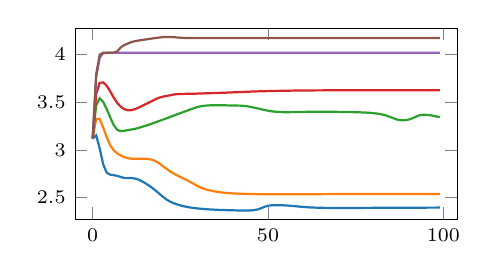
\begin{tikzpicture}

\definecolor{crimson2143940}{RGB}{214,39,40}
\definecolor{darkgray176}{RGB}{176,176,176}
\definecolor{darkorange25512714}{RGB}{255,127,14}
\definecolor{forestgreen4416044}{RGB}{44,160,44}
\definecolor{mediumpurple148103189}{RGB}{148,103,189}
\definecolor{sienna1408675}{RGB}{140,86,75}
\definecolor{steelblue31119180}{RGB}{31,119,180}

\begin{axis}[compar]
\addplot [thick, steelblue31119180]
table {%
0 3.11796808242798
1 3.15118432044983
2 3.01552939414978
3 2.84774732589722
4 2.75995588302612
5 2.73878240585327
6 2.73351860046387
7 2.72573399543762
8 2.71427464485168
9 2.70477652549744
10 2.70237755775452
11 2.70297002792358
12 2.69900965690613
13 2.68789911270142
14 2.67062258720398
15 2.64913964271545
16 2.62546396255493
17 2.59937429428101
18 2.57031655311584
20 2.50738406181335
21 2.4793426990509
22 2.4574179649353
23 2.44052267074585
24 2.42700123786926
25 2.41591334342957
26 2.40676498413086
27 2.39922213554382
28 2.39300632476807
29 2.38787364959717
30 2.38361406326294
32 2.37704825401306
34 2.37229657173157
36 2.36874318122864
39 2.36492252349854
42 2.36257195472717
44 2.36234927177429
45 2.36335945129395
46 2.36629676818848
47 2.37319493293762
48 2.38594627380371
49 2.40138411521912
50 2.41227293014526
51 2.41700339317322
52 2.41823697090149
54 2.41712141036987
55 2.41559243202209
56 2.41324472427368
58 2.40651035308838
60 2.39966654777527
62 2.39470195770264
64 2.39169883728027
66 2.3901059627533
69 2.38922643661499
75 2.38944745063782
99 2.39285945892334
};

\addplot [thick, darkorange25512714]
table {%
0 3.11796808242798
1 3.32535791397095
2 3.3224675655365
3 3.23482942581177
4 3.13118267059326
5 3.0477180480957
6 2.99429082870483
7 2.96304988861084
8 2.94067072868347
9 2.92288279533386
10 2.91210031509399
11 2.90701508522034
12 2.90518188476562
15 2.90581560134888
16 2.90258741378784
17 2.89445948600769
18 2.8795325756073
19 2.85680174827576
21 2.8011839389801
22 2.77524399757385
23 2.75248837471008
24 2.73251247406006
26 2.69666624069214
27 2.67861199378967
28 2.65926241874695
30 2.61770915985107
31 2.60020995140076
32 2.58697628974915
33 2.57683110237122
34 2.56862735748291
35 2.56180000305176
36 2.55609250068665
37 2.55135631561279
38 2.54747796058655
40 2.54188013076782
42 2.53842425346375
45 2.53533840179443
49 2.53283500671387
53 2.5319995880127
58 2.53272151947021
70 2.53503847122192
83 2.53560161590576
99 2.53566694259644
};
\addplot [thick, forestgreen4416044]
table {%
0 3.11796808242798
1 3.4686393737793
2 3.5406768321991
3 3.50344061851501
4 3.42863726615906
5 3.34067630767822
6 3.25861430168152
7 3.20941400527954
8 3.19578289985657
9 3.19926619529724
10 3.20650839805603
12 3.21937322616577
13 3.22884202003479
16 3.26350712776184
17 3.27625799179077
19 3.30341982841492
21 3.32977271080017
24 3.37187623977661
29 3.43887281417847
30 3.4503927230835
31 3.45823550224304
32 3.46309113502502
33 3.46610140800476
34 3.46790051460266
35 3.46873712539673
37 3.46801257133484
40 3.46501088142395
42 3.46394968032837
43 3.46171116828918
44 3.45720791816711
45 3.45082831382751
47 3.43512225151062
49 3.41795372962952
50 3.41029024124146
51 3.40455055236816
52 3.40044093132019
53 3.39748907089233
54 3.39571332931519
55 3.39501857757568
57 3.39576458930969
62 3.39940118789673
65 3.39978313446045
69 3.39886236190796
73 3.39677405357361
76 3.39388060569763
78 3.3905827999115
79 3.3881983757019
80 3.38505887985229
81 3.38084435462952
82 3.37508583068848
83 3.36713671684265
84 3.35630202293396
85 3.34250068664551
86 3.32768893241882
87 3.31598830223083
88 3.31031775474548
89 3.31077694892883
90 3.31670331954956
91 3.32823538780212
92 3.34492540359497
93 3.36041283607483
94 3.36738705635071
95 3.36783909797668
96 3.36432266235352
97 3.3579638004303
99 3.3426308631897
};
\addplot [thick, crimson2143940]
table {%
0 3.11796808242798
1 3.58576369285583
2 3.70367240905762
3 3.70745038986206
4 3.67220902442932
5 3.61500382423401
6 3.54777121543884
7 3.49231767654419
8 3.45297169685364
9 3.42684817314148
10 3.41456604003906
11 3.41643738746643
12 3.42613506317139
13 3.44117450714111
15 3.47795104980469
16 3.49490284919739
17 3.51290106773376
18 3.53240847587585
19 3.54803562164307
20 3.55762982368469
22 3.57209539413452
23 3.57982659339905
24 3.58468818664551
25 3.58658170700073
29 3.58927297592163
38 3.60024666786194
46 3.61276125907898
52 3.61830830574036
57 3.62173199653625
62 3.6237211227417
69 3.62495470046997
82 3.6255362033844
99 3.62563323974609
};
\addplot [thick, mediumpurple148103189]
table {%
0 3.11796808242798
1 3.76111364364624
2 3.96444940567017
3 4.01592350006104
4 4.01859855651855
16 4.0185546875
99 4.0185546875
};
\addplot [thick, sienna1408675]
table {%
0 3.11796808242798
1 3.79262447357178
2 3.99938130378723
3 4.01962184906006
5 4.01985263824463
6 4.02090549468994
7 4.03304672241211
8 4.07537746429443
9 4.09999942779541
10 4.11583471298218
11 4.13082981109619
12 4.14075517654419
13 4.1471791267395
18 4.1749062538147
20 4.18352460861206
21 4.18583583831787
22 4.18560981750488
23 4.18328380584717
25 4.17733287811279
26 4.17544078826904
28 4.17417287826538
69 4.17432069778442
99 4.17432069778442
};
\end{axis}

\end{tikzpicture}
}
&
\multicolumn{4}{c}{% This file was created with tikzplotlib v0.10.1.
\begin{tikzpicture}

\definecolor{crimson2143940}{RGB}{214,39,40}
\definecolor{darkgray176}{RGB}{176,176,176}
\definecolor{darkorange25512714}{RGB}{255,127,14}
\definecolor{forestgreen4416044}{RGB}{44,160,44}
\definecolor{mediumpurple148103189}{RGB}{148,103,189}
\definecolor{sienna1408675}{RGB}{140,86,75}
\definecolor{steelblue31119180}{RGB}{31,119,180}

\begin{axis}[
height=\figheight,
tick align=outside,
tick pos=left,
width=\figwidth,
x grid style={darkgray176},
xmin=-4.95, xmax=103.95,
xtick style={color=black},
y grid style={darkgray176},
ymin=8.98000025749207, ymax=15.139999628067,
ytick style={color=black}
]
\addplot [semithick, steelblue31119180]
table {%
0 13.5699996948242
1 13.8599996566772
2 14.210000038147
3 14.4899997711182
4 14.5200004577637
5 14.4200000762939
6 14.3299999237061
9 14.1499996185303
10 14.1099996566772
11 14.0799999237061
12 14.0699996948242
13 14.0900001525879
17 14.25
18 14.3000001907349
19 14.3599996566772
21 14.5
22 14.5600004196167
24 14.6599998474121
25 14.6999998092651
26 14.7299995422363
27 14.75
28 14.7799997329712
29 14.789999961853
30 14.8100004196167
34 14.8500003814697
35 14.8500003814697
36 14.8599996566772
41 14.8599996566772
44 14.8299999237061
45 14.8100004196167
46 14.7700004577637
47 14.710000038147
48 14.6199998855591
49 14.5100002288818
50 14.4300003051758
51 14.3900003433228
52 14.3699998855591
55 14.3400001525879
58 14.3400001525879
61 14.3699998855591
62 14.3699998855591
63 14.3800001144409
69 14.3800001144409
70 14.3699998855591
73 14.3699998855591
74 14.3599996566772
77 14.3599996566772
78 14.3500003814697
81 14.3500003814697
82 14.3400001525879
88 14.3400001525879
89 14.3299999237061
97 14.3299999237061
98 14.3199996948242
99 12.8999996185303
};
\addplot [semithick, darkorange25512714]
table {%
0 13.210000038147
1 13.0500001907349
2 13.0600004196167
4 13.2799997329712
5 13.3400001525879
6 13.3699998855591
7 13.3800001144409
8 13.3599996566772
9 13.3199996948242
11 13.2799997329712
12 13.2799997329712
13 13.289999961853
14 13.3100004196167
16 13.3299999237061
17 13.3299999237061
18 13.3400001525879
19 13.3800001144409
22 13.5600004196167
24 13.6599998474121
26 13.7399997711182
28 13.8400001525879
30 13.960000038147
34 14.1199998855591
37 14.1800003051758
40 14.210000038147
50 14.210000038147
51 14.1999998092651
56 14.1999998092651
57 14.1899995803833
61 14.1899995803833
62 14.1800003051758
74 14.1800003051758
75 14.1700000762939
81 14.1700000762939
82 14.1800003051758
98 14.1800003051758
99 12.8699998855591
};
\addplot [semithick, forestgreen4416044]
table {%
0 12.8500003814697
1 12.3199996948242
2 12.1499996185303
3 12.1800003051758
4 12.2299995422363
6 12.3500003814697
7 12.3199996948242
8 12.210000038147
9 12.1300001144409
10 12.1000003814697
12 12.0600004196167
13 12.0299997329712
15 11.9499998092651
16 11.9200000762939
19 11.7700004577637
20 11.7399997711182
21 11.6999998092651
23 11.6400003433228
24 11.6000003814697
28 11.4799995422363
30 11.3999996185303
31 11.3800001144409
33 11.3599996566772
34 11.3599996566772
35 11.3500003814697
37 11.3500003814697
38 11.3599996566772
41 11.3599996566772
44 11.3900003433228
45 11.4200000762939
46 11.4399995803833
47 11.4700002670288
48 11.5100002288818
49 11.539999961853
50 11.5799999237061
52 11.6400003433228
53 11.6599998474121
54 11.6899995803833
57 11.7200002670288
64 11.7200002670288
65 11.710000038147
69 11.710000038147
70 11.6999998092651
79 11.6999998092651
80 11.710000038147
81 11.710000038147
83 11.7299995422363
84 11.75
86 11.7700004577637
88 11.7700004577637
89 11.7799997329712
90 11.7799997329712
92 11.8000001907349
93 11.8000001907349
94 11.789999961853
96 11.8100004196167
98 11.8500003814697
99 10.789999961853
};
\addplot [semithick, crimson2143940]
table {%
0 12.5100002288818
1 11.6700000762939
2 11.3999996185303
3 11.3599996566772
4 11.3900003433228
5 11.4300003051758
6 11.460000038147
7 11.5
8 11.5200004577637
9 11.5299997329712
11 11.4300003051758
12 11.3900003433228
13 11.3400001525879
14 11.2700004577637
17 11.1199998855591
18 11.0500001907349
19 10.9899997711182
20 10.9499998092651
22 10.8900003433228
23 10.8500003814697
24 10.8199996948242
25 10.8100004196167
26 10.789999961853
27 10.7799997329712
29 10.7399997711182
33 10.6999998092651
35 10.6999998092651
36 10.6899995803833
38 10.6899995803833
39 10.6800003051758
41 10.6800003051758
42 10.6700000762939
46 10.6700000762939
47 10.6599998474121
54 10.6599998474121
55 10.6499996185303
73 10.6499996185303
74 10.6400003433228
98 10.6400003433228
99 9.90999984741211
};
\addplot [semithick, mediumpurple148103189]
table {%
0 11.8400001525879
1 10.5600004196167
2 10.1099996566772
3 10
4 9.98999977111816
98 9.98999977111816
99 9.81999969482422
};
\addplot [semithick, sienna1408675]
table {%
0 11.6999998092651
1 10.3299999237061
2 9.88000011444092
3 9.82999992370605
5 9.82999992370605
6 9.81999969482422
7 9.77000045776367
8 9.59000015258789
9 9.48999977111816
10 9.4399995803833
11 9.40999984741211
12 9.39000034332275
13 9.38000011444092
14 9.35999965667725
15 9.35000038146973
16 9.32999992370605
17 9.31999969482422
18 9.30000019073486
19 9.28999996185303
20 9.28999996185303
21 9.27999973297119
23 9.27999973297119
24 9.28999996185303
32 9.28999996185303
33 9.27999973297119
98 9.27999973297119
99 9.26000022888184
};
\end{axis}

\end{tikzpicture}
}
\end{tabular}
    \caption{Comparaison de la PGD avec le résultat attendu (Target) après 100 itérations et avec différent pas --- initialisation $^tA(Ax)$, passe-bas gaussien ($\sigma=0.6$)}
\end{figure}




\newpage



\section{Conclusion}

Par manque de temps, il n'a pas été trop possible de trop rentrer dans la théorie mais au vue des résultats il est clair que qu'il y a quelque chose à voir.  
\\
Il a été fait le choix de de supposer $f_D$ inversible pour exprimer le fait que $f_D$ vienne qu'un auto-encodeur. Mais peut-être qu'une formalisation moins dur, pas exemple en terme de voisinage, de cette idée pourrait être moins restrictive. En particulier, avoir $\ d\big(\theta, \theta^*\big)=\big\|\theta-\theta^*\big\|_2\ $ plutôt qu'une égalité permettrait d'élargir le bassin $\Lambda_\beta$, ce qui serait plus cohérent avec les résultats
\\

A voir sur des images plus complexes mais \apriori, les modèles très résistant à l'aliasing




\newpage





\begin{annexe}
\section{Annexes}

\subsection{Auto-encodeur}\label{anx:AE}
\quad

Comme expliqué en début de rapport, section \ref{sec:forma2pb}, les auto-encodeurs utilisés, sont des réseaux MLP comptant une couche cachée de taille 1500 pour les parties encodage et décodage, et d'espace latent de taille respective 100, 200, 400 et 800. Pour reprendre ce qui a été fait par Peng \etal, tout les fonctions d'activations sont des sigmoïdes, ce qui, retrospectivement, n'était pas le plus judicieux (\cf section \ref{sec:article1/2}).
\\
Leur entraînement s'est fait sur le jeu de données MNIST sur 60 epochs avec des batchs de tailles 100.  Il est effectué par le code \texttt{training autoencoder.py} disponible sur le  \href{https://www.youtube.com/watch?v=dQw4w9WgXcQ&pp=ygUIcmlja3JvbGw%3D}{GitHub} et dont voici un résumé des performances :
\\
\begin{figure}[H]\centering
    \setlength{\tabcolsep}{3pt}
\begin{tabular}{ c c c c c c c c c }

\rotatebox[origin=lt]{90}{Input}
&
\includegraphics[width=0.115\textwidth]{resultats/auto-encoder/AE-100_1_input.png}
&
\includegraphics[width=0.115\textwidth]{resultats/auto-encoder/AE-100_2_input.png}
&
\includegraphics[width=0.115\textwidth]{resultats/auto-encoder/AE-100_3_input.png}
&
\includegraphics[width=0.115\textwidth]{resultats/auto-encoder/AE-100_4_input.png}
&
\includegraphics[width=0.115\textwidth]{resultats/auto-encoder/AE-100_5_input.png}
&
\includegraphics[width=0.115\textwidth]{resultats/auto-encoder/AE-100_6_input.png}
&
\includegraphics[width=0.115\textwidth]{resultats/auto-encoder/AE-100_7_input.png}
&
\includegraphics[width=0.115\textwidth]{resultats/auto-encoder/AE-100_8_input.png}

\\ %\hline

\rotatebox[origin=lt]{90}{\quad\ }
&
{\scriptsize PSNR=28.74}
&
{\scriptsize PSNR=29.68}
&
{\scriptsize PSNR=26.2}
&
{\scriptsize PSNR=29.65}
&
{\scriptsize PSNR=26.76}
&
{\scriptsize PSNR=28.69}
&
{\scriptsize PSNR=28.41}
&
{\scriptsize PSNR=27.76}

\\

\rotatebox[origin=lt]{90}{\ \ 100}
&
\includegraphics[width=0.115\textwidth]{resultats/auto-encoder/AE-100_1_PSNR=28.74_output.png}
&
\includegraphics[width=0.115\textwidth]{resultats/auto-encoder/AE-100_2_PSNR=29.68_output.png}
&
\includegraphics[width=0.115\textwidth]{resultats/auto-encoder/AE-100_3_PSNR=26.2_output.png}
&
\includegraphics[width=0.115\textwidth]{resultats/auto-encoder/AE-100_4_PSNR=29.65_output.png}
&
\includegraphics[width=0.115\textwidth]{resultats/auto-encoder/AE-100_5_PSNR=26.76_output.png}
&
\includegraphics[width=0.115\textwidth]{resultats/auto-encoder/AE-100_6_PSNR=28.69_output.png}
&
\includegraphics[width=0.115\textwidth]{resultats/auto-encoder/AE-100_7_PSNR=28.41_output.png}
&
\includegraphics[width=0.115\textwidth]{resultats/auto-encoder/AE-100_8_PSNR=27.76_output.png}

\\

\rotatebox[origin=lt]{90}{\quad\ }
&
{\scriptsize PSNR=29.64}
&
{\scriptsize PSNR=29.24}
&
{\scriptsize PSNR=27.29}
&
{\scriptsize PSNR=30.21}
&
{\scriptsize PSNR=28.16}
&
{\scriptsize PSNR=29.71}
&
{\scriptsize PSNR=30.85}
&
{\scriptsize PSNR=29.12}

\\

\rotatebox[origin=lt]{90}{\ \ 200}
&
\includegraphics[width=0.115\textwidth]{resultats/auto-encoder/AE-200_1_PSNR=29.64_output.png}
&
\includegraphics[width=0.115\textwidth]{resultats/auto-encoder/AE-200_2_PSNR=29.24_output.png}
&
\includegraphics[width=0.115\textwidth]{resultats/auto-encoder/AE-200_3_PSNR=27.29_output.png}
&
\includegraphics[width=0.115\textwidth]{resultats/auto-encoder/AE-200_4_PSNR=30.21_output.png}
&
\includegraphics[width=0.115\textwidth]{resultats/auto-encoder/AE-200_5_PSNR=28.16_output.png}
&
\includegraphics[width=0.115\textwidth]{resultats/auto-encoder/AE-200_6_PSNR=29.71_output.png}
&
\includegraphics[width=0.115\textwidth]{resultats/auto-encoder/AE-200_7_PSNR=30.85_output.png}
&
\includegraphics[width=0.115\textwidth]{resultats/auto-encoder/AE-200_8_PSNR=29.12_output.png}

\\

\rotatebox[origin=lt]{90}{\quad\ }
&
{\scriptsize PSNR=30.28}
&
{\scriptsize PSNR=30.76}
&
{\scriptsize PSNR=27.43}
&
{\scriptsize PSNR=30.53}
&
{\scriptsize PSNR=29.54}
&
{\scriptsize PSNR=29.83}
&
{\scriptsize PSNR=31.53}
&
{\scriptsize PSNR=31.3}

\\

\rotatebox[origin=lt]{90}{\ \ 400}
&
\includegraphics[width=0.115\textwidth]{resultats/auto-encoder/AE-400_1_PSNR=30.28_output.png}
&
\includegraphics[width=0.115\textwidth]{resultats/auto-encoder/AE-400_2_PSNR=30.76_output.png}
&
\includegraphics[width=0.115\textwidth]{resultats/auto-encoder/AE-400_3_PSNR=27.43_output.png}
&
\includegraphics[width=0.115\textwidth]{resultats/auto-encoder/AE-400_4_PSNR=30.53_output.png}
&
\includegraphics[width=0.115\textwidth]{resultats/auto-encoder/AE-400_5_PSNR=29.54_output.png}
&
\includegraphics[width=0.115\textwidth]{resultats/auto-encoder/AE-400_6_PSNR=29.83_output.png}
&
\includegraphics[width=0.115\textwidth]{resultats/auto-encoder/AE-400_7_PSNR=31.53_output.png}
&
\includegraphics[width=0.115\textwidth]{resultats/auto-encoder/AE-400_8_PSNR=31.3_output.png}

\end{tabular}
    \caption{Reconstruction par auto-encodeur des images Input en fonction de la taille de l'espace latent du dit auto-encodeur et avec les PSNR associés}
    \label{fig:AEapp}
\end{figure}
\begin{figure}[H]\centering
    \setlength{\tabcolsep}{0pt}
\begin{tabular}{r r r r r}

& &  Autoencoder 100{\color{white}bbbb}  &  Autoencoder 200{\color{white}bbbb}  &  Autoencoder 400{\color{white}bbbb}  

\\ \\

\rotatebox[origin=lt]{90}{{\color{white}bbbb}MSE}
& &
% This file was created with tikzplotlib v0.10.1.
\begin{tikzpicture}

\definecolor{darkgray176}{RGB}{176,176,176}
\definecolor{darkorange25512714}{RGB}{255,127,14}
\definecolor{steelblue31119180}{RGB}{31,119,180}

\begin{axis}[
height=\figheight,
log basis y={10},
tick align=outside,
tick pos=left,
width=\figwidth,
x grid style={darkgray176},
xmin=-2.95, xmax=61.95,
xtick style={color=black},
y grid style={darkgray176},
ymin=0.00165886754046576, ymax=0.0611124005692584,
ymode=log,
ytick style={color=black},
ytick={0.0001,0.001,0.01,0.1,1},
yticklabels={
  \(\displaystyle {10^{-4}}\),
  \(\displaystyle {10^{-3}}\),
  \(\displaystyle {10^{-2}}\),
  \(\displaystyle {10^{-1}}\),
  \(\displaystyle {10^{0}}\)
}
]
\addplot [semithick, steelblue31119180]
table {%
0 0.0518720038235188
1 0.02554801851511
2 0.0173378624022007
3 0.0133188515901566
4 0.0109316576272249
5 0.00939567107707262
6 0.00828651990741491
7 0.00748166767880321
8 0.00685237208381295
9 0.00635064486414194
10 0.00591443525627255
11 0.00555017963051796
12 0.00523966317996383
13 0.00495978863909841
14 0.00473269680514932
15 0.00453824829310179
17 0.00418460322543979
18 0.00404801033437252
19 0.00392276374623179
20 0.00379281048662961
21 0.00368099054321647
22 0.00356699386611581
23 0.00348103558644652
25 0.00329699576832354
26 0.00322135980241001
27 0.00314237107522786
29 0.00301361549645662
30 0.00294889183714986
31 0.00289292447268963
32 0.00283385463990271
33 0.00278664077632129
35 0.00268257665447891
37 0.00258983112871647
38 0.00255701458081603
40 0.00246976083144546
43 0.00236683199182153
44 0.00234519876539707
45 0.00229926710017025
48 0.00221881736069918
49 0.00219219038262963
50 0.00215819384902716
54 0.00206096656620502
55 0.00204216712154448
57 0.00199954304844141
58 0.0019717204850167
59 0.00195437553338706
};
\addplot [semithick, darkorange25512714]
table {%
0 0.0330518148839474
1 0.0198523905128241
2 0.0147118531167507
3 0.0115565303713083
4 0.00981095712631941
5 0.00865060556679964
6 0.00774995889514685
7 0.00707322917878628
8 0.00661052903160453
9 0.00609223870560527
10 0.00581139419227839
11 0.00543221551924944
12 0.00516849244013429
13 0.00497076008468866
15 0.00457627838477492
16 0.0044299834407866
17 0.00435137096792459
18 0.00418223068118095
19 0.00410104729235172
20 0.00395805621519685
21 0.00384121690876782
23 0.00369861349463463
24 0.00358767551369965
25 0.00353957526385784
26 0.00343360542319715
27 0.00338863302022219
28 0.00336424726992846
29 0.00330294319428504
30 0.00326295848935843
31 0.00318127800710499
33 0.00310822506435215
34 0.00310828490182757
35 0.0030126660130918
36 0.00301306950859725
37 0.00297222589142621
38 0.00297658750787377
39 0.00283884350210428
40 0.00284207612276077
41 0.00281827640719712
42 0.00277460599318147
43 0.00275322678498924
44 0.00274799601174891
45 0.00271018617786467
46 0.00267772865481675
47 0.00265605910681188
48 0.00262555666267872
49 0.0026655406691134
50 0.00257417652755976
51 0.00255639688111842
52 0.00255104713141918
53 0.00251109828241169
54 0.0024961472954601
55 0.00248667155392468
56 0.00245288014411926
57 0.0024546233471483
58 0.00243026949465275
59 0.0024220822378993
};
\end{axis}

\end{tikzpicture}

&
% This file was created with tikzplotlib v0.10.1.
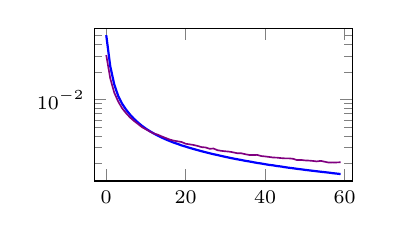
\begin{tikzpicture}

\definecolor{darkgray176}{RGB}{176,176,176}
\definecolor{darkorange25512714}{RGB}{255,127,14}
\definecolor{steelblue31119180}{RGB}{31,119,180}

\begin{axis}[speAE,
ymode=log,
ytick={0.0001,0.001,0.01,0.1,1},
yticklabels={
  \(\displaystyle {10^{-4}}\),
  \(\displaystyle {10^{-3}}\),
  \(\displaystyle {10^{-2}}\),
  \(\displaystyle {10^{-1}}\),
  \(\displaystyle {10^{0}}\)
}
]
\addplot [thick, blue]
table {%
0 0.0503827184438705
1 0.0231762751936913
2 0.014697564765811
3 0.0109478253871202
4 0.00899229943752289
5 0.00774224475026131
6 0.00684232404455543
7 0.00614844681695104
8 0.00560816191136837
9 0.00516596203669906
10 0.00480720214545727
11 0.00450789043679833
12 0.00425539258867502
13 0.00403159903362393
14 0.00384168932214379
15 0.00366993132047355
16 0.00352168921381235
17 0.00338485115207732
18 0.00327525730244815
19 0.00315655907616019
20 0.00306433159857988
21 0.00296860747039318
23 0.00280534545890987
24 0.00272952229715884
26 0.0025950912386179
27 0.00253195920959115
28 0.00247928220778704
29 0.00242134579457343
31 0.00231824209913611
33 0.00222833012230694
34 0.00218915846198797
35 0.00214463635347784
36 0.00211104960180819
38 0.00203325902111828
39 0.00200548488646746
40 0.00196877960115671
41 0.00193660240620375
42 0.00191451469436288
43 0.00188098242506385
44 0.00185941788367927
45 0.00182812963612378
46 0.00180087820626795
47 0.0017799154156819
48 0.00175378890708089
49 0.001733677694574
50 0.00170948228333145
54 0.00162926164921373
56 0.00159461738076061
57 0.00157220743130893
58 0.00155619683209807
59 0.00153788621537387
};
\addplot [semithick, violet]
table {%
0 0.0305683203041553
1 0.017071396112442
2 0.011926488019526
3 0.00952861737459898
4 0.0080207260325551
5 0.00709329778328538
6 0.00636689830571413
7 0.0058362390846014
8 0.00540540693327785
9 0.00499403430148959
11 0.0044674351811409
12 0.00425342144444585
13 0.00413477141410112
14 0.00395425315946341
16 0.00365695520304143
17 0.00355988088995218
18 0.0035015782341361
19 0.00343526271171868
20 0.0032912774477154
21 0.00324278487823904
22 0.00319049344398081
23 0.00311692943796515
24 0.00302586634643376
25 0.00299932225607336
26 0.00290136504918337
27 0.00292090233415365
28 0.00279996660538018
29 0.00275404471904039
30 0.00272374297492206
31 0.0027005102019757
32 0.00265146419405937
33 0.00259227468632162
34 0.00259035988710821
35 0.00253120018169284
36 0.00248397560790181
37 0.00248199491761625
38 0.0024878759868443
39 0.00241875112988055
40 0.00239369249902666
41 0.00236381567083299
42 0.00233046384528279
43 0.00232217158190906
44 0.00229623098857701
45 0.00228002434596419
46 0.00228015333414078
47 0.0022583685349673
48 0.00218693865463138
49 0.00219371449202299
50 0.00216764211654663
51 0.00215686019510031
52 0.00213886913843453
53 0.0021116673015058
54 0.00214252411387861
56 0.00205086614005268
57 0.00205984897911549
58 0.00205883500166237
59 0.00206905510276556
};
\end{axis}

\end{tikzpicture}

&
% This file was created with tikzplotlib v0.10.1.
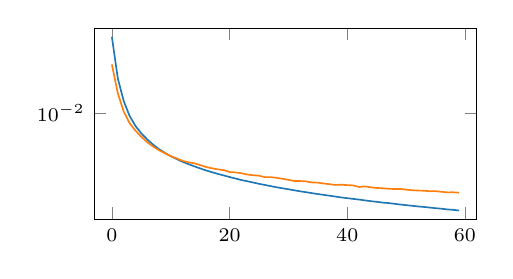
\begin{tikzpicture}

\definecolor{darkgray176}{RGB}{176,176,176}
\definecolor{darkorange25512714}{RGB}{255,127,14}
\definecolor{steelblue31119180}{RGB}{31,119,180}

\begin{axis}[compar,
	ymode=log]
\addplot [semithick, steelblue31119180]
table {%
0 0.0492035262286663
1 0.0207414887845516
2 0.0129387434571981
3 0.00945419538766146
4 0.00766767701134086
5 0.00656204577535391
6 0.00578529853373766
7 0.00518497824668884
8 0.00472294026985765
9 0.00436683231964707
10 0.00407265918329358
12 0.00362355192191899
14 0.00329436152242124
16 0.00302357808686793
18 0.0028144761454314
20 0.00263713044114411
22 0.00247619464062154
23 0.0024149629753083
25 0.00228715874254704
28 0.00212763133458793
30 0.00204079411923885
32 0.00195532198995352
35 0.00184639461804181
36 0.00181616784539074
37 0.00178282673005015
38 0.00175259064417332
39 0.00171963183674961
41 0.00166981155052781
42 0.00164510158356279
44 0.00159098510630429
45 0.00157107796985656
46 0.00154567917343229
47 0.00153023435268551
49 0.00148346740752459
50 0.00146513234358281
52 0.00142524391412735
53 0.00141107453964651
55 0.00137436343356967
56 0.00136018230114132
57 0.00134005874861032
58 0.00132755958475173
59 0.00130976806394756
};
\addplot [semithick, darkorange25512714]
table {%
0 0.0276999436318874
1 0.0152005106210709
2 0.0103711616247892
3 0.00814399775117636
4 0.00693845562636852
5 0.00611581327393651
6 0.00544816395267844
7 0.00498418230563402
8 0.00461689289659262
9 0.00433709705248475
10 0.0040805097669363
11 0.00389086711220443
12 0.00370007567107677
13 0.00358308735303581
14 0.00351104489527643
15 0.00338523765094578
16 0.00325000286102295
17 0.00316429394297302
18 0.00309449038468301
19 0.00304547790437937
20 0.00292374682612717
21 0.00290122651495039
22 0.00285399938002229
23 0.00277612800709903
24 0.00273615051992238
25 0.00271024717949331
26 0.00262898951768875
27 0.0026314384303987
28 0.00259054196067154
29 0.00254159467294812
30 0.00248572020791471
31 0.00242716423235834
32 0.00242336583323777
33 0.00240683532319963
34 0.0023516824003309
35 0.00234355125576258
36 0.00229976209811866
37 0.00226869224570692
38 0.00223404658026993
39 0.00224652979522943
40 0.00222630659118295
41 0.00221177469938993
42 0.00214156811125576
43 0.00216725165955722
44 0.00212531164288521
45 0.00209872331470251
46 0.0020835162140429
47 0.00206287042237818
48 0.0020514854695648
49 0.00205233367159963
50 0.00202494696713984
51 0.00200132979080081
52 0.00198752526193857
53 0.00198013707995415
54 0.00196109595708549
55 0.00196250132285058
57 0.00191261433064938
58 0.00191620655823499
59 0.00189937290269881
};
\end{axis}

\end{tikzpicture}


\\

\rotatebox[origin=lt]{90}{{\color{white}bbbb}PSNR}
& &
% This file was created with tikzplotlib v0.10.1.
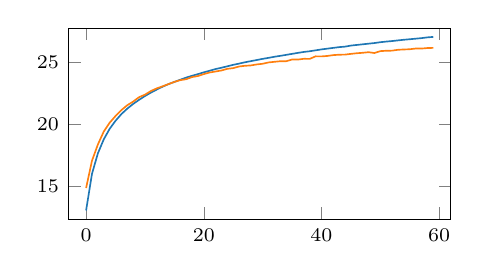
\begin{tikzpicture}

\definecolor{darkgray176}{RGB}{176,176,176}
\definecolor{darkorange25512714}{RGB}{255,127,14}
\definecolor{steelblue31119180}{RGB}{31,119,180}

\begin{axis}[compar]
\addplot [semithick, steelblue31119180]
table {%
0 12.9921646118164
1 15.9709796905518
2 17.6316299438477
3 18.7714214324951
4 19.6243877410889
5 20.2814331054688
6 20.825569152832
7 21.2693367004395
8 21.6509838104248
9 21.9818019866943
10 22.290246963501
11 22.5658435821533
12 22.8153610229492
13 23.0541896820068
14 23.2580280303955
15 23.4398918151855
17 23.7910099029541
18 23.9354858398438
19 24.0712852478027
20 24.2189025878906
21 24.3479061126709
22 24.4848308563232
23 24.5913696289062
25 24.826379776001
26 24.9274959564209
27 25.0352840423584
29 25.2175579071045
30 25.3115119934082
31 25.3935966491699
32 25.4829597473145
33 25.556453704834
36 25.7987403869629
37 25.8744373321533
38 25.9299793243408
40 26.0803718566895
43 26.2660179138184
44 26.3055362701416
45 26.3908996582031
48 26.5458984375
49 26.5972957611084
50 26.6657619476318
51 26.715425491333
52 26.7595901489258
54 26.8653030395508
55 26.9054412841797
57 26.9971542358398
58 27.0580635070801
59 27.0958271026611
};
\addplot [semithick, darkorange25512714]
table {%
0 14.8166589736938
1 17.0394096374512
2 18.3499698638916
3 19.4052104949951
4 20.12087059021
5 20.6666812896729
6 21.1473579406738
7 21.5459537506104
8 21.8410625457764
9 22.1983013153076
10 22.4017715454102
11 22.6959228515625
12 22.9133548736572
13 23.081262588501
15 23.4413452148438
16 23.5824241638184
17 23.658863067627
18 23.8318309783936
19 23.9167766571045
20 24.0732536315918
21 24.2038154602051
23 24.3677520751953
24 24.5024852752686
25 24.5585422515869
26 24.6924247741699
27 24.7486114501953
28 24.7782421112061
29 24.8595581054688
30 24.9125595092773
31 25.0220222473145
33 25.1214275360107
34 25.1195774078369
35 25.2583465576172
36 25.2555713653564
37 25.3172721862793
38 25.3094215393066
39 25.5182762145996
40 25.5110721588135
41 25.5484962463379
42 25.6167793273926
43 25.6492214202881
44 25.6571216583252
45 25.7165641784668
46 25.7686500549316
47 25.8048152923584
48 25.8545074462891
49 25.786994934082
50 25.9404563903809
51 25.9712791442871
52 25.9788265228271
53 26.0497512817383
54 26.0743026733398
55 26.0925235748291
56 26.1517753601074
57 26.1480541229248
58 26.1905174255371
59 26.2049503326416
};
\end{axis}

\end{tikzpicture}

&
% This file was created with tikzplotlib v0.10.1.
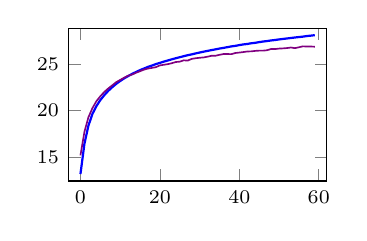
\begin{tikzpicture}

\definecolor{darkgray176}{RGB}{176,176,176}
\definecolor{darkorange25512714}{RGB}{255,127,14}
\definecolor{steelblue31119180}{RGB}{31,119,180}

\begin{axis}[speAE
]
\addplot [thick, blue]
table {%
0 13.141565322876
1 16.4121437072754
2 18.3559398651123
3 19.6229076385498
4 20.4739570617676
5 21.121940612793
6 21.6586933135986
7 22.1230201721191
8 22.5214576721191
9 22.8782615661621
10 23.190357208252
11 23.4693088531494
12 23.7187671661377
13 23.9537391662598
14 24.1627216339111
15 24.3614559173584
17 24.7117385864258
18 24.8552265167236
19 25.0149211883545
20 25.1446475982666
21 25.2817459106445
23 25.5281562805176
24 25.6464061737061
26 25.8652076721191
27 25.9728870391846
28 26.0626010894775
29 26.1668891906738
31 26.3553466796875
33 26.5267696380615
34 26.6037197113037
35 26.6926212310791
36 26.7621040344238
38 26.9245300292969
39 26.9842643737793
40 27.0646324157715
41 27.1359672546387
42 27.1858768463135
43 27.2623500823975
44 27.3123149871826
45 27.3857326507568
46 27.4515209197998
47 27.502025604248
48 27.5662307739258
49 27.6161918640137
50 27.6774291992188
54 27.8856678009033
56 27.9792156219482
57 28.0409603118896
58 28.0852375030518
59 28.1366901397705
};
\addplot [semithick, violet]
table {%
0 15.1579599380493
1 17.7009410858154
2 19.2677421569824
3 20.2477607727051
4 21.000602722168
5 21.5357780456543
6 22.0056056976318
7 22.3844528198242
8 22.7170639038086
9 23.0631332397461
11 23.5465240478516
12 23.761116027832
13 23.8813629150391
14 24.0759983062744
16 24.4174518585205
17 24.5327701568604
18 24.6020584106445
19 24.686107635498
20 24.8729763031006
22 25.0086402893066
23 25.1091575622559
24 25.2393856048584
25 25.2758560180664
26 25.4226875305176
27 25.3897819519043
28 25.5762500762939
29 25.6475467681885
30 25.6960620880127
31 25.7340679168701
32 25.8129272460938
33 25.9113426208496
34 25.9128532409668
35 26.0150375366211
36 26.0973606109619
37 26.0996189117432
38 26.0877342224121
39 26.2120475769043
40 26.2576656341553
41 26.3121719360352
42 26.3743019104004
43 26.388822555542
44 26.4381885528564
45 26.4681549072266
46 26.4669132232666
47 26.5092792510986
48 26.650764465332
49 26.6363906860352
50 26.6879081726074
51 26.709623336792
52 26.7456436157227
53 26.8024978637695
54 26.7362613677979
55 26.830005645752
56 26.9311370849609
57 26.9100170135498
58 26.911470413208
59 26.8904571533203
};
\end{axis}

\end{tikzpicture}

&
% This file was created with tikzplotlib v0.10.1.
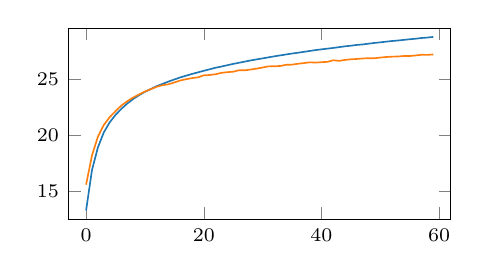
\begin{tikzpicture}

\definecolor{darkgray176}{RGB}{176,176,176}
\definecolor{darkorange25512714}{RGB}{255,127,14}
\definecolor{steelblue31119180}{RGB}{31,119,180}

\begin{axis}[compar]
\addplot [semithick, steelblue31119180]
table {%
0 13.2728042602539
1 16.8960628509521
2 18.9158535003662
3 20.2616062164307
4 21.1672916412354
5 21.8417053222656
6 22.3864879608154
7 22.8624649047852
8 23.2667961120605
9 23.6068515777588
10 23.9097938537598
12 24.4168853759766
14 24.8300304412842
16 25.2024040222168
18 25.5130214691162
20 25.7950820922852
22 26.0686435699463
23 26.1776180267334
25 26.4130954742432
28 26.7272052764893
30 26.9088249206543
32 27.0939693450928
35 27.3428802490234
36 27.413818359375
39 27.651948928833
40 27.7185516357422
42 27.8439426422119
44 27.9892120361328
45 28.0439777374268
46 28.1142082214355
47 28.157564163208
49 28.2926139831543
50 28.3467178344727
52 28.4665489196777
53 28.5100154876709
55 28.6242618560791
56 28.6696815490723
57 28.73388671875
58 28.7748146057129
59 28.8332748413086
};
\addplot [semithick, darkorange25512714]
table {%
0 15.5871000289917
1 18.2080001831055
2 19.8783931732178
3 20.9324569702148
4 21.6307258605957
5 22.1794261932373
6 22.6829452514648
7 23.0694847106934
8 23.4025821685791
10 23.9384956359863
11 24.1459331512451
12 24.3642425537109
13 24.5037326812744
14 24.5904636383057
15 24.7491874694824
16 24.9271564483643
17 25.0406379699707
18 25.1383953094482
19 25.2085819244385
20 25.3868732452393
21 25.417516708374
22 25.4887542724609
23 25.6104412078857
24 25.6722221374512
25 25.7123947143555
26 25.8468799591064
27 25.840425491333
28 25.910120010376
29 25.9917697906494
30 26.0894184112549
31 26.1942081451416
32 26.1996917724609
33 26.2298202514648
34 26.3323268890381
35 26.3461246490479
36 26.4279403686523
37 26.4865188598633
38 26.5542278289795
39 26.528959274292
40 26.5687160491943
41 26.5965518951416
42 26.738151550293
43 26.6855964660645
44 26.7709846496582
45 26.8254051208496
46 26.8574275970459
47 26.9000606536865
48 26.9245586395264
49 26.922248840332
50 26.9806575775146
51 27.0315456390381
52 27.0615119934082
53 27.0784149169922
54 27.1207332611084
55 27.1165866851807
57 27.2284736633301
58 27.2209587097168
59 27.2595596313477
};
\end{axis}

\end{tikzpicture}

\end{tabular}
    \caption{Évolution de la MSE et du PSNR par batch des auto-encodeurs au cours des epochs. En bleu sur le set d'entraînement et en violet sur celui de test}
    \label{fig:AEperf}
\end{figure}
%\\ \\



\subsection{Calcul pratique de $\bf{F}$ et de son gradient}\label{anx:gradF}
\quad

\begin{enonce}[Notation ({\normalfont pas sur qu'il y en ait besoin}]
Comme $A$ est linéaire, dans toute la suite elle sera assimilé à matrice la représentant. Là où l'opérateur $A$ prend pour entrée un image $\bf{x}\in\R^{n\times m}$, sa représentation matricielle elle prendre un vecteur $x\in\R^{nm}$. Par souci de lisibilité on notera dans toute la suite les images sous forme d'image en gras, leur version vectoriel en fin avec l'abus de notation :
\[A(\bf{x})=Ax\]

\emph{Ces notations seront également valable pour toute autre opérateur linéaire.}
\end{enonce}

Le fait de supposer $A$ linéaire permet de calcul explicitement le gradient de $F$ à moindre coût :
\begin{equation}\label{eq:gradient}
\forall x\in\R^{nm},\qquad \nabla F(x)=\,^tA\big(Ax-y\big)
\end{equation}{\color{white}l}
Si la formule (\ref{eq:gradient}) est mathématiquement très simple, dès que $n$ et $m$ seront un peu trop grand, la taille de $A$ va très vite ralentir tout algorithme de descente, voir rendre impossible son stockage en mémoire.

Pour y remédier, notons $\F$ (resp. $\F^{-1}$) la matrice associée à la transformée (resp. inverse) de Fourier discrète. En notant de plus $\hat{\bf{x}}=\F \bf{x}$ et $\odot$ le produit terme à terme de vecteur/matrice, $A$ s'écrit alors :
\begin{align*}\forall \bf{x}\in\R^{n\times m},\qquad A(\bf{x})=S\circ C_h(\bf{x})=S(\bf{h}*\bf{x})&=S\circ\F^{-1}\F(\bf{h}*\bf{x})\\
    &=S\circ\F^{-1}\big(\hat{\bf{h}}\odot\hat{\bf{x}}\big)\end{align*}
\\
La transformé de Fourier discrète étant symétrique\footnote{comme $x$ a été aplatie, $\F$ n'est pas diagonale à proprement parler, nous y revenons plus loin} et $D_h$ aussi (car diagonale), le gradient de $F$ se réécrire comme :
\begin{align*}\forall x\in\R^{nm},\qquad \nabla F(x)=\,^tA\big(Ax-y\big)&=\,^t\Big(S\F^{-1}D_h\F\Big)\big(S\F^{-1}D_h\F x-y\big)\\
    &=\,^t\F\,^tD_h\,^t\F^{-1}\,^tS\big(S\F^{-1}D_h\F x-y\big)\\
    &=\F D_h\F^{-1}\,^tS\big(S\F^{-1}D_h\F x-y\big)\end{align*}
\\
Sous cette forme et même s'il n'en n'a pas l'air, le gradient est bien plus simple à calculer et rapide à calculer.

D'abord, la projection $S$ est très peu coûteuse en temps de calcul puisqu'elle consiste à ne garder qu'un certain nombre de pixel de l'image. Par exemple, la  \figref{fig:Simg} ci-dessous représente une image $4\times 3$ sous-échantillonnée en une image $2\times2$  et du point de vu matricielle, $S$ prend la forme de la \figref{fig:Smat}.

Du point de vu python, cela revient simplement à ne conserver qu'une valeur sur deux dans le tableau que représente l'image. De façon plus générale, la projection $S$ se traduit par la commande : 
\[\forall x\in\R^{n\times m},\qquad S(x):=\texttt{Sx = x[::n//p, ::m//q]}\]
\begin{figure}[H]\centering
    %\input{figures/matrice S}
\end{figure}
\noindent
Avec ces représentation, on se convainc sans trop de difficulté qu'appliquer la transposé $^tS$ à une image $y\in\R^{p\times q}$ revient reprendre un antécédent de $y$ par $S$ et à remplacer les valeurs des pixels qui ne sont pas conserver par $S$ par des 0. Cette manipulation ne demande pas non plus de construire $^tS$, il suffit de produit une image $^tSy=$\pyt{tSy} de taille $(n,m)$ remplie de 0 et d'ensuite faire la modification :
\[\forall (i,j)\in\llbracket1,p\rrbracket\times\llbracket1,q\rrbracket,\qquad \texttt{tSy[i*n//p, j*p//q] = y[i,j]}\]
\\
Dans notre cas, $n=m=28$ et pour le moment $p=q=14$. Le code reste néanmoins relativement flexible de ce point de vue la puisqu'il devrait marcher tant que $p$ (resp. $q$) divise $n$ (resp. $m$), \emph{plus de détail dans le code}. La \figref{fig:sousechanti} ci-dessous montre les applications successives de $S$ et $^tS$ une image $x$.
\begin{figure}[H]\centering
    %\begin{tabular}{l c c c l c c c l}
$x$ & & & & $Sx$ & & & & $^tS(Sx)$
\\

\includegraphics[width=0.25\textwidth]{resultats/compare_filter/seed21-x.png}
& & & &
\includegraphics[width=0.25\textwidth]{resultats/compare_filter/seed21-Ax-filtre=s.png}
& & & &
\includegraphics[width=0.25\textwidth]{resultats/compare_filter/seed21-tA(Ax)-filtre=s.png}\end{tabular}
    \caption{SENSING MATRIX --- Application du sous-échantillonnage à une image, puis application sa transposé}
    \label{fig:sousechanti}
\end{figure}

\begin{figure}[H]\centering
    %\begin{tabular}{c c c c c c}

$\sigma=0.3$  &  $\sigma=0.4$  &  $\sigma=0.5$  &  $\sigma=0.6$  &  $\sigma=0.7$ & $\sigma=0.8$

\\

\includegraphics[width=0.14\textwidth]{resultats/compare_filter/seed21-f-filtre=g_param=0.3.png}
&
\includegraphics[width=0.14\textwidth]{resultats/compare_filter/seed21-f-filtre=g_param=0.4.png}
&
\includegraphics[width=0.14\textwidth]{resultats/compare_filter/seed21-f-filtre=g_param=0.5.png}
&
\includegraphics[width=0.14\textwidth]{resultats/compare_filter/seed21-f-filtre=g_param=0.6.png}
&
\includegraphics[width=0.14\textwidth]{resultats/compare_filter/seed21-f-filtre=g_param=0.7.png}
&
\includegraphics[width=0.14\textwidth]{resultats/compare_filter/seed21-f-filtre=g_param=0.8.png}

\\

\includegraphics[width=0.14\textwidth]{resultats/compare_filter/seed21-x.png}
&
\includegraphics[width=0.14\textwidth]{resultats/compare_filter/seed21-x.png}
&
\includegraphics[width=0.14\textwidth]{resultats/compare_filter/seed21-x.png}
&
\includegraphics[width=0.14\textwidth]{resultats/compare_filter/seed21-x.png}
&
\includegraphics[width=0.14\textwidth]{resultats/compare_filter/seed21-x.png}
&
\includegraphics[width=0.14\textwidth]{resultats/compare_filter/seed21-x.png}

\\

\includegraphics[width=0.14\textwidth]{resultats/compare_filter/seed21-Ax-filtre=g_param=0.3.png}
&
\includegraphics[width=0.14\textwidth]{resultats/compare_filter/seed21-Ax-filtre=g_param=0.4.png}
&
\includegraphics[width=0.14\textwidth]{resultats/compare_filter/seed21-Ax-filtre=g_param=0.5.png}
&
\includegraphics[width=0.14\textwidth]{resultats/compare_filter/seed21-Ax-filtre=g_param=0.6.png}
&
\includegraphics[width=0.14\textwidth]{resultats/compare_filter/seed21-Ax-filtre=g_param=0.7.png}
&
\includegraphics[width=0.14\textwidth]{resultats/compare_filter/seed21-Ax-filtre=g_param=0.8.png}

\\

\includegraphics[width=0.14\textwidth]{resultats/compare_filter/seed21-tA(Ax)-filtre=g_param=0.3.png}
&
\includegraphics[width=0.14\textwidth]{resultats/compare_filter/seed21-tA(Ax)-filtre=g_param=0.4.png}
&
\includegraphics[width=0.14\textwidth]{resultats/compare_filter/seed21-tA(Ax)-filtre=g_param=0.5.png}
&
\includegraphics[width=0.14\textwidth]{resultats/compare_filter/seed21-tA(Ax)-filtre=g_param=0.6.png}
&
\includegraphics[width=0.14\textwidth]{resultats/compare_filter/seed21-tA(Ax)-filtre=g_param=0.7.png}
&
\includegraphics[width=0.14\textwidth]{resultats/compare_filter/seed21-tA(Ax)-filtre=g_param=0.8.png}
\end{tabular}
    
    \caption{En première ligne la transformé du filtres  $\hat{\bf{h}}$ gaussien d'écart type $\sigma$, en deuxième l'image $\bf{x}$ ($28\times28$), en troisième le résultat $A(\bf{x})$ ($14\times14$) et en dernière ligne le produit $tA(A\bf{x})$ ($28\times28$).}
    \label{fig:passebas-g}
\end{figure}

\begin{figure}[H]\centering
    \begin{tabular}{c c c c c c}
$a=0.9$  &  $a=0.75$  &  $a=0.6$  &  $a=0.4$  &  $a=0.25$ & $a=0.1$

\\

\includegraphics[width=0.14\textwidth]{resultats/compare_filter/seed21-f-filtre=p_param=0.9.png}
&
\includegraphics[width=0.14\textwidth]{resultats/compare_filter/seed21-f-filtre=p_param=0.75.png}
&
\includegraphics[width=0.14\textwidth]{resultats/compare_filter/seed21-f-filtre=p_param=0.6.png}
&
\includegraphics[width=0.14\textwidth]{resultats/compare_filter/seed21-f-filtre=p_param=0.4.png}
&
\includegraphics[width=0.14\textwidth]{resultats/compare_filter/seed21-f-filtre=p_param=0.25.png}
&
\includegraphics[width=0.14\textwidth]{resultats/compare_filter/seed21-f-filtre=p_param=0.1.png}
\\ \\



\includegraphics[width=0.14\textwidth]{resultats/compare_filter/seed21-x.png}
&
\includegraphics[width=0.14\textwidth]{resultats/compare_filter/seed21-x.png}
&
\includegraphics[width=0.14\textwidth]{resultats/compare_filter/seed21-x.png}
&
\includegraphics[width=0.14\textwidth]{resultats/compare_filter/seed21-x.png}
&
\includegraphics[width=0.14\textwidth]{resultats/compare_filter/seed21-x.png}
&
\includegraphics[width=0.14\textwidth]{resultats/compare_filter/seed21-x.png}
\\ \\



\includegraphics[width=0.14\textwidth]{resultats/compare_filter/seed21-Ax-filtre=p_param=0.9.png}
&
\includegraphics[width=0.14\textwidth]{resultats/compare_filter/seed21-Ax-filtre=p_param=0.75.png}
&
\includegraphics[width=0.14\textwidth]{resultats/compare_filter/seed21-Ax-filtre=p_param=0.6.png}
&
\includegraphics[width=0.14\textwidth]{resultats/compare_filter/seed21-Ax-filtre=p_param=0.4.png}
&
\includegraphics[width=0.14\textwidth]{resultats/compare_filter/seed21-Ax-filtre=p_param=0.25.png}
&
\includegraphics[width=0.14\textwidth]{resultats/compare_filter/seed21-Ax-filtre=p_param=0.1.png}
\\ \\



\includegraphics[width=0.14\textwidth]{resultats/compare_filter/seed21-tA(Ax)-filtre=p_param=0.9.png}
&
\includegraphics[width=0.14\textwidth]{resultats/compare_filter/seed21-tA(Ax)-filtre=p_param=0.75.png}
&
\includegraphics[width=0.14\textwidth]{resultats/compare_filter/seed21-tA(Ax)-filtre=p_param=0.6.png}
&
\includegraphics[width=0.14\textwidth]{resultats/compare_filter/seed21-tA(Ax)-filtre=p_param=0.4.png}
&
\includegraphics[width=0.14\textwidth]{resultats/compare_filter/seed21-tA(Ax)-filtre=p_param=0.25.png}
&
\includegraphics[width=0.14\textwidth]{resultats/compare_filter/seed21-tA(Ax)-filtre=p_param=0.1.png}
\end{tabular}
    \caption{Idem qu'à la figure \ref{fig:passebas-g} avec cette fois $\hat{\bf{h}}$ qui est l'indicatrice de $[-a,a]\times[-a,a]$}
    \label{fig:passebas-p}
\end{figure}
%\\ \\




\subsection{Ancien résultats}

\begin{figure}[H]\centering
    %\begin{tabular}{c c c}

Image cible $\bf{x_0}$  &  Image reconstruite par PGD  &  Évolution de $F$

\\

\includegraphics[width=0.25\textwidth]{resultats (legacy)/PGD/no-h-target-pas=1e-20_filtre=s-None.png}
&
\includegraphics[width=0.25\textwidth]{resultats (legacy)/PGD/no-h-guess-pas=1e-20_filtre=s-None.png}&
% This file was created with tikzplotlib v0.10.1.
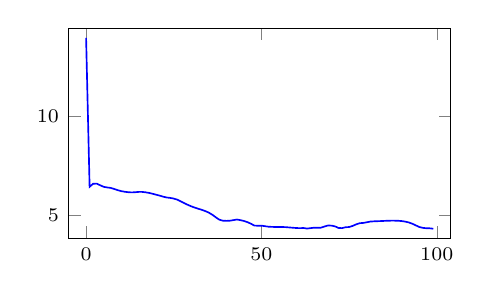
\begin{tikzpicture}

\definecolor{darkgray176}{RGB}{176,176,176}

\begin{axis}[standard, legend pos=north west]
\addplot [semithick, blue]
table {%
0 14.0099983215332
1 6.43522930145264
2 6.59043264389038
3 6.59941053390503
4 6.51600074768066
5 6.43675327301025
6 6.40419435501099
7 6.38027667999268
8 6.32742691040039
9 6.26683378219604
10 6.21821737289429
11 6.18551206588745
12 6.16198205947876
13 6.15156936645508
14 6.1617226600647
15 6.17761039733887
16 6.17704629898071
17 6.15684223175049
18 6.12322807312012
19 6.08116388320923
21 5.98693561553955
22 5.93357801437378
23 5.89308929443359
24 5.87161827087402
25 5.83802127838135
26 5.78176355361938
27 5.69534349441528
28 5.60409545898438
29 5.520188331604
30 5.44388818740845
31 5.37805986404419
33 5.26488447189331
34 5.20181274414062
35 5.12310218811035
36 5.01670932769775
37 4.88474035263062
38 4.7662467956543
39 4.7140417098999
40 4.70628833770752
41 4.71348333358765
43 4.77372455596924
44 4.74268054962158
45 4.70022630691528
46 4.64184999465942
47 4.56022310256958
48 4.46469259262085
49 4.45909929275513
50 4.46086502075195
52 4.40946865081787
53 4.39968776702881
54 4.39535903930664
56 4.3943042755127
57 4.38481044769287
59 4.35486078262329
60 4.34218454360962
61 4.33439064025879
62 4.34463787078857
63 4.31305122375488
65 4.3593430519104
66 4.35771656036377
67 4.35996007919312
68 4.41990423202515
69 4.47263622283936
70 4.46255826950073
71 4.42429113388062
72 4.3442554473877
73 4.33725786209106
74 4.38228511810303
75 4.39282178878784
76 4.4487681388855
77 4.5274224281311
78 4.58700895309448
79 4.60040712356567
80 4.63313817977905
81 4.66963052749634
82 4.68143701553345
84 4.69541025161743
86 4.71262836456299
87 4.716224193573
88 4.71557998657227
89 4.70952987670898
90 4.69506549835205
91 4.66848564147949
92 4.62566471099854
93 4.56127405166626
95 4.39467430114746
96 4.35059928894043
97 4.3303427696228
98 4.32735109329224
99 4.30526828765869
};
\end{axis}

\end{tikzpicture}


\\ \\

Image cible compressée $A(\bf{x_0})$  &  Initialisation de la PGD  & Évolution de PSNR

\\

\includegraphics[width=0.25\textwidth]{resultats (legacy)/PGD/no-h-comptarg-pas=1e-20_filtre=s-None.png}
&
\includegraphics[width=0.25\textwidth]{resultats (legacy)/PGD/no-h-init-pas=1e-20_filtre=s-None.png}
&
% This file was created with tikzplotlib v0.10.1.
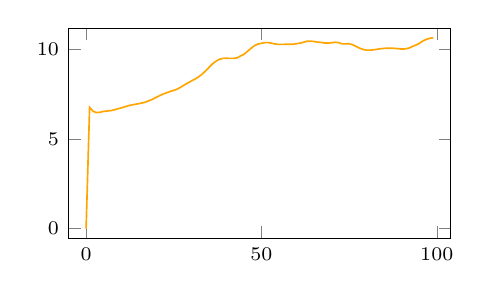
\begin{tikzpicture}

\definecolor{darkgray176}{RGB}{176,176,176}
\definecolor{orange}{RGB}{255,165,0}

\begin{axis}[standard]
\addplot [semithick, orange]
table {%
0 -0
1 6.76999998092651
2 6.53999996185303
3 6.46999979019165
4 6.48999977111816
5 6.53999996185303
7 6.57999992370605
8 6.61999988555908
9 6.67999982833862
10 6.73000001907349
12 6.84999990463257
13 6.90000009536743
14 6.92999982833862
16 7.01000022888184
17 7.05999994277954
19 7.21999979019165
21 7.42000007629395
22 7.51000022888184
24 7.65000009536743
25 7.71000003814697
26 7.78000020980835
27 7.8899998664856
28 8.01000022888184
30 8.22999954223633
31 8.32999992370605
32 8.44999980926514
33 8.60000038146973
34 8.77999973297119
36 9.18000030517578
37 9.32999992370605
38 9.4399995803833
39 9.48999977111816
40 9.5
41 9.48999977111816
42 9.48999977111816
43 9.52000045776367
45 9.72000026702881
46 9.88000011444092
47 10.0500001907349
48 10.1999998092651
49 10.289999961853
51 10.3699998855591
52 10.3699998855591
54 10.289999961853
55 10.2700004577637
56 10.2700004577637
57 10.2799997329712
59 10.2799997329712
61 10.3400001525879
62 10.3900003433228
63 10.4499998092651
64 10.4499998092651
65 10.4300003051758
66 10.3999996185303
67 10.3800001144409
68 10.3500003814697
69 10.3500003814697
70 10.3599996566772
71 10.3900003433228
72 10.3699998855591
73 10.3000001907349
74 10.3000001907349
75 10.3100004196167
76 10.25
77 10.1599998474121
78 10.0600004196167
79 9.98999977111816
80 9.94999980926514
81 9.94999980926514
82 9.97000026702881
84 10.0299997329712
85 10.0500001907349
86 10.0600004196167
87 10.0600004196167
88 10.0500001907349
90 10.0100002288818
91 10.0200004577637
92 10.0600004196167
93 10.1499996185303
94 10.2299995422363
95 10.3299999237061
96 10.460000038147
97 10.5500001907349
98 10.6099996566772
99 10.6400003433228
};
\end{axis}

\end{tikzpicture}


\end{tabular}
    \caption{Résultat de la PGD avec un pas de descente $\rho=10^{-20}$, sans filtre passe-bas}
\end{figure}

\begin{figure}[H]\centering
    %\begin{tabular}{c c c c c c}
Target  &  $(1)$  &  $(2)$  &  $(3)$  &  $(4)$

\\

\multirow{2}{0.3\textwidth}[0.125\textwidth]{\includegraphics[width=0.3\textwidth]{resultats (legacy)/LGD/comp-inits-s21-target-pas=0.05_filtre=s-None.png}}
&
\includegraphics[width=0.15\textwidth]{resultats (legacy)/LGD/comp-inits-s21_1-init-pas=0.05_filtre=s-None.png}
&
\includegraphics[width=0.15\textwidth]{resultats (legacy)/LGD/comp-inits-s21_2-init-pas=0.05_filtre=s-None.png}
&
\includegraphics[width=0.15\textwidth]{resultats (legacy)/LGD/comp-inits-s21_3-init-pas=0.05_filtre=s-None.png}
&
\includegraphics[width=0.15\textwidth]{resultats (legacy)/LGD/comp-inits-s21_4-init-pas=0.05_filtre=s-None.png}

\\


&
\includegraphics[width=0.15\textwidth]{resultats (legacy)/LGD/comp-inits-s21_1-guess-pas=0.05_filtre=s-None.png}
&
\includegraphics[width=0.15\textwidth]{resultats (legacy)/LGD/comp-inits-s21_2-guess-pas=0.05_filtre=s-None.png}
&
\includegraphics[width=0.15\textwidth]{resultats (legacy)/LGD/comp-inits-s21_3-guess-pas=0.05_filtre=s-None.png}
&
\includegraphics[width=0.15\textwidth]{resultats (legacy)/LGD/comp-inits-s21_4-guess-pas=0.05_filtre=s-None.png}

\\ \\



\multicolumn{2}{c}{Loss}  &  \multicolumn{3}{c}{PSNR}

\\

\multicolumn{2}{c}{% This file was created with tikzplotlib v0.10.1.
\begin{tikzpicture}

\definecolor{crimson2143940}{RGB}{214,39,40}
\definecolor{darkgray176}{RGB}{176,176,176}
\definecolor{darkorange25512714}{RGB}{255,127,14}
\definecolor{forestgreen4416044}{RGB}{44,160,44}
\definecolor{steelblue31119180}{RGB}{31,119,180}

\begin{axis}[
height=\figheight,
tick align=outside,
tick pos=left,
width=\figwidth,
x grid style={darkgray176},
xmin=-4.95, xmax=103.95,
xtick style={color=black},
y grid style={darkgray176},
ymin=-0.0579753056168557, ymax=7.15792880803347,
ytick style={color=black}
]
\addplot [semithick, steelblue31119180]
table {%
0 4.00298118591309
1 3.36831521987915
2 2.91190457344055
3 2.6143946647644
4 2.37283110618591
5 2.21564602851868
6 2.13336992263794
7 2.10726809501648
9 2.07294702529907
10 2.04974746704102
11 2.01104927062988
13 1.88066112995148
14 1.85316371917725
15 1.83743119239807
18 1.80224740505219
20 1.78404426574707
25 1.74990999698639
26 1.73262751102448
27 1.69542860984802
28 1.61424350738525
29 1.53965759277344
30 1.52243995666504
32 1.50793087482452
34 1.49561297893524
35 1.4866818189621
36 1.47224199771881
37 1.44414126873016
38 1.37981784343719
39 1.25765383243561
40 1.19188845157623
41 1.17538917064667
42 1.16487073898315
44 1.15114760398865
49 1.12455713748932
50 1.11573159694672
51 1.10193777084351
52 1.07663822174072
53 1.02107536792755
54 0.887021899223328
55 0.695062041282654
56 0.630431175231934
57 0.610252141952515
58 0.599629878997803
60 0.588108777999878
63 0.579365730285645
68 0.571701526641846
78 0.562842726707458
94 0.548416376113892
99 0.539865612983704
};
\addplot [semithick, darkorange25512714]
table {%
0 6.82993316650391
1 4.85147428512573
2 3.59235715866089
3 2.99921369552612
4 2.50282120704651
5 2.10352516174316
6 1.8378643989563
7 1.66291701793671
8 1.50895118713379
9 1.42252147197723
10 1.38319051265717
11 1.35853028297424
12 1.34072363376617
14 1.31554388999939
17 1.28877627849579
19 1.27126836776733
20 1.26034200191498
21 1.24583005905151
22 1.22438085079193
23 1.19003450870514
24 1.13679373264313
25 1.07734978199005
26 1.04335224628448
27 1.03015375137329
29 1.01952707767487
32 1.01207756996155
38 1.00419449806213
48 0.997184753417969
65 0.990990161895752
98 0.984931945800781
99 0.984782338142395
};
\addplot [semithick, forestgreen4416044]
table {%
0 2.26342844963074
1 1.13021111488342
2 0.828698635101318
3 0.721487760543823
4 0.657673120498657
7 0.489104747772217
8 0.439910650253296
9 0.401624798774719
10 0.37336790561676
11 0.35236668586731
12 0.336367011070251
13 0.323922157287598
15 0.306454539299011
17 0.295873522758484
20 0.287751317024231
25 0.282615065574646
37 0.277874231338501
64 0.272974610328674
99 0.270020365715027
};
\addplot [semithick, crimson2143940]
table {%
0 4.15597200393677
1 3.87473487854004
2 3.60465502738953
3 3.36457109451294
4 3.16414904594421
5 2.99086809158325
7 2.66685509681702
8 2.50774812698364
9 2.35596394538879
10 2.21620440483093
11 2.08985352516174
12 1.97613954544067
13 1.87381160259247
14 1.78178215026855
15 1.69908845424652
16 1.62474489212036
17 1.55773675441742
18 1.49709582328796
19 1.44196903705597
20 1.39163422584534
21 1.34548795223236
22 1.30302202701569
23 1.26380217075348
24 1.22745263576508
26 1.16207575798035
28 1.10465502738953
30 1.05340123176575
32 1.00689303874969
35 0.943720817565918
38 0.886392593383789
41 0.833761096000671
44 0.785638093948364
47 0.742311000823975
50 0.70404589176178
53 0.670785188674927
56 0.642127752304077
60 0.610037565231323
64 0.583585500717163
69 0.556546330451965
74 0.534505605697632
80 0.512871503829956
87 0.492423892021179
96 0.471413254737854
99 0.465391278266907
};
\end{axis}

\end{tikzpicture}
}
&
\multicolumn{3}{c}{% This file was created with tikzplotlib v0.10.1.
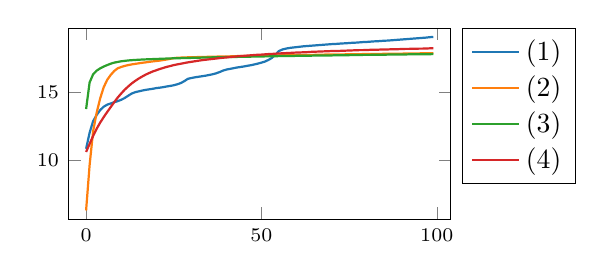
\begin{tikzpicture}

\definecolor{crimson2143940}{RGB}{214,39,40}
\definecolor{darkgray176}{RGB}{176,176,176}
\definecolor{darkorange25512714}{RGB}{255,127,14}
\definecolor{forestgreen4416044}{RGB}{44,160,44}
\definecolor{steelblue31119180}{RGB}{31,119,180}

\begin{axis}[compar, legend pos=outer north east]
\addplot [thick, steelblue31119180]
table {%
0 10.8299999237061
1 12.0100002288818
2 12.8599996566772
3 13.3100004196167
4 13.6700000762939
5 13.9200000762939
6 14.0699996948242
8 14.25
9 14.3299999237061
10 14.4300003051758
11 14.5600004196167
12 14.7299995422363
13 14.8900003433228
14 14.9899997711182
16 15.1099996566772
17 15.1599998474121
19 15.2399997711182
20 15.289999961853
21 15.3199996948242
22 15.3599996566772
23 15.4099998474121
24 15.4499998092651
25 15.5
26 15.5699996948242
27 15.6599998474121
28 15.8000001907349
29 15.9700002670288
30 16.0300006866455
31 16.0799999237061
34 16.2000007629395
36 16.2999992370605
37 16.3700008392334
38 16.4599990844727
39 16.5699996948242
40 16.6499996185303
43 16.7999992370605
45 16.8799991607666
46 16.9300003051758
47 16.9699993133545
49 17.0900001525879
50 17.1599998474121
51 17.2399997711182
52 17.3600006103516
53 17.5100002288818
54 17.75
55 18.0100002288818
56 18.1299991607666
57 18.1900005340576
58 18.2399997711182
62 18.3600006103516
70 18.5200004577637
71 18.5300006866455
73 18.5699996948242
74 18.5799999237061
76 18.6200008392334
77 18.6299991607666
79 18.6700000762939
80 18.6800003051758
82 18.7199993133545
83 18.7299995422363
85 18.7700004577637
86 18.7800006866455
97 19
98 19.0300006866455
99 19.0499992370605
};
\addlegendentry{$(1)$}
\addplot [thick, darkorange25512714]
table {%
0 6.30000019073486
1 9.63000011444092
2 12.1199998855591
3 13.4700002670288
4 14.5200004577637
5 15.3400001525879
6 15.8900003433228
7 16.25
8 16.5400009155273
9 16.7399997711182
10 16.8400001525879
11 16.9200000762939
12 16.9799995422363
13 17.0300006866455
16 17.1499996185303
17 17.1800003051758
18 17.2199993133545
21 17.3099994659424
23 17.3899993896484
25 17.4899997711182
26 17.5200004577637
30 17.5599994659424
31 17.5599994659424
33 17.5799999237061
34 17.5799999237061
35 17.5900001525879
36 17.5900001525879
38 17.6100006103516
39 17.6100006103516
40 17.6200008392334
41 17.6200008392334
43 17.6399993896484
44 17.6399993896484
45 17.6499996185303
46 17.6499996185303
47 17.6599998474121
48 17.6599998474121
49 17.6700000762939
50 17.6700000762939
51 17.6800003051758
53 17.6800003051758
54 17.6900005340576
55 17.6900005340576
56 17.7000007629395
57 17.7000007629395
58 17.7099990844727
60 17.7099990844727
61 17.7199993133545
62 17.7199993133545
63 17.7299995422363
65 17.7299995422363
66 17.7399997711182
67 17.7399997711182
68 17.75
70 17.75
71 17.7600002288818
73 17.7600002288818
74 17.7700004577637
75 17.7700004577637
76 17.7800006866455
78 17.7800006866455
79 17.7900009155273
81 17.7900009155273
82 17.7999992370605
84 17.7999992370605
85 17.8099994659424
87 17.8099994659424
88 17.8199996948242
90 17.8199996948242
91 17.8299999237061
93 17.8299999237061
94 17.8400001525879
95 17.8400001525879
96 17.8500003814697
98 17.8500003814697
99 17.8600006103516
};
\addlegendentry{$(2)$}
\addplot [thick, forestgreen4416044]
table {%
0 13.75
1 15.6999998092651
2 16.2999992370605
3 16.5699996948242
4 16.7399997711182
5 16.8700008392334
6 16.9799995422363
7 17.0799999237061
8 17.1599998474121
10 17.2600002288818
12 17.3199996948242
14 17.3600006103516
15 17.3700008392334
16 17.3899993896484
25 17.4799995422363
26 17.4799995422363
28 17.5
29 17.5
31 17.5200004577637
32 17.5200004577637
33 17.5300006866455
34 17.5300006866455
36 17.5499992370605
37 17.5499992370605
38 17.5599994659424
39 17.5599994659424
40 17.5699996948242
41 17.5699996948242
42 17.5799999237061
43 17.5799999237061
44 17.5900001525879
45 17.5900001525879
46 17.6000003814697
47 17.6000003814697
48 17.6100006103516
50 17.6100006103516
51 17.6200008392334
52 17.6200008392334
53 17.6299991607666
54 17.6299991607666
55 17.6399993896484
57 17.6399993896484
58 17.6499996185303
59 17.6499996185303
60 17.6599998474121
62 17.6599998474121
63 17.6700000762939
64 17.6700000762939
65 17.6800003051758
67 17.6800003051758
68 17.6900005340576
70 17.6900005340576
71 17.7000007629395
73 17.7000007629395
74 17.7099990844727
75 17.7099990844727
76 17.7199993133545
78 17.7199993133545
79 17.7299995422363
81 17.7299995422363
82 17.7399997711182
85 17.7399997711182
86 17.75
88 17.75
89 17.7600002288818
91 17.7600002288818
92 17.7700004577637
94 17.7700004577637
95 17.7800006866455
98 17.7800006866455
99 17.7900009155273
};
\addlegendentry{$(3)$}
\addplot [thick, crimson2143940]
table {%
0 10.6000003814697
1 11.1899995803833
2 11.7700004577637
3 12.3000001907349
4 12.75
5 13.1499996185303
6 13.5299997329712
8 14.25
9 14.5900001525879
10 14.8900003433228
11 15.1700000762939
12 15.4099998474121
13 15.6300001144409
14 15.8199996948242
15 15.9899997711182
16 16.1399993896484
17 16.2800006866455
18 16.3999996185303
19 16.5100002288818
21 16.6900005340576
23 16.8500003814697
24 16.9099998474121
25 16.9799995422363
29 17.1800003051758
33 17.3400001525879
39 17.5200004577637
40 17.5400009155273
41 17.5699996948242
42 17.5900001525879
43 17.6200008392334
49 17.7399997711182
50 17.75
52 17.7900009155273
53 17.7999992370605
54 17.8199996948242
55 17.8299999237061
56 17.8500003814697
58 17.8700008392334
59 17.8899993896484
63 17.9300003051758
64 17.9500007629395
71 18.0200004577637
72 18.0200004577637
78 18.0799999237061
79 18.0799999237061
82 18.1100006103516
83 18.1100006103516
85 18.1299991607666
86 18.1299991607666
88 18.1499996185303
89 18.1499996185303
91 18.1700000762939
92 18.1700000762939
93 18.1800003051758
94 18.1800003051758
95 18.1900005340576
96 18.1900005340576
98 18.2099990844727
99 18.2099990844727
};
\addlegendentry{$(4)$}
\end{axis}

\end{tikzpicture}
}
\end{tabular}
    \caption{ PGD --- En première lignes différentes initialisation avec en dessous le résultats de la PGD après 100 itérations --- $\rho=10^{-20}$ sans passe-bas}
    \label{fig:1}
\end{figure}

\begin{figure}[H]\centering
    %\begin{tabular}{c c c c c c}
Aléatoire  &  Aléat + AE  &  $^tA(\bf{y_0})$  & $\bf{x_0}+$bruit ($0.01$)  & $\bf{x_0}+$bruit ($0.001$)  & $\bf{x_0}+$bruit ($0.0001$) 

\\


%% This file was created with tikzplotlib v0.10.1.
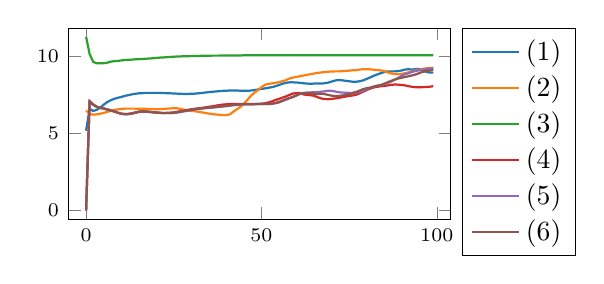
\begin{tikzpicture}

\definecolor{crimson2143940}{RGB}{214,39,40}
\definecolor{darkgray176}{RGB}{176,176,176}
\definecolor{darkorange25512714}{RGB}{255,127,14}
\definecolor{forestgreen4416044}{RGB}{44,160,44}
\definecolor{mediumpurple148103189}{RGB}{148,103,189}
\definecolor{sienna1408675}{RGB}{140,86,75}
\definecolor{steelblue31119180}{RGB}{31,119,180}

\begin{axis}[compar, legend pos=outer north east]
\addplot [thick, steelblue31119180]
table {%
0 5.15999984741211
1 6.57999992370605
2 6.44000005722046
3 6.51000022888184
4 6.65000009536743
5 6.84000015258789
6 7.01000022888184
7 7.13000011444092
8 7.21999979019165
9 7.28999996185303
10 7.34000015258789
11 7.40999984741211
13 7.51000022888184
14 7.55000019073486
15 7.57999992370605
16 7.59000015258789
17 7.6100001335144
21 7.6100001335144
28 7.53999996185303
29 7.53999996185303
31 7.55999994277954
33 7.59999990463257
35 7.65999984741211
39 7.73999977111816
42 7.76999998092651
45 7.73999977111816
46 7.73999977111816
47 7.76000022888184
48 7.78999996185303
49 7.82999992370605
50 7.8600001335144
53 7.98000001907349
54 8.03999996185303
56 8.19999980926514
57 8.26000022888184
58 8.28999996185303
59 8.28999996185303
60 8.27999973297119
61 8.26000022888184
62 8.22999954223633
63 8.21000003814697
64 8.19999980926514
65 8.21000003814697
67 8.21000003814697
68 8.22999954223633
69 8.27000045776367
71 8.40999984741211
72 8.4399995803833
73 8.42000007629395
76 8.32999992370605
77 8.32999992370605
78 8.35999965667725
79 8.42000007629395
80 8.51000022888184
82 8.71000003814697
83 8.80000019073486
85 8.96000003814697
86 9
88 9
89 9.02000045776367
90 9.0600004196167
91 9.11999988555908
92 9.14000034332275
93 9.10999965667725
94 9.15999984741211
95 9.14999961853027
97 8.97000026702881
98 8.92000007629395
99 8.92000007629395
};
\addlegendentry{$(1)$}
\addplot [thick, darkorange25512714]
table {%
0 6.46999979019165
1 6.23999977111816
2 6.19999980926514
3 6.21999979019165
4 6.26000022888184
5 6.30999994277954
6 6.38000011444092
8 6.5
9 6.53999996185303
10 6.57000017166138
11 6.59000015258789
14 6.59000015258789
15 6.57999992370605
17 6.57999992370605
20 6.55000019073486
22 6.57000017166138
23 6.59000015258789
24 6.59999990463257
25 6.61999988555908
26 6.6100001335144
27 6.57000017166138
28 6.51000022888184
29 6.46999979019165
30 6.44000005722046
31 6.42000007629395
32 6.3899998664856
35 6.26999998092651
37 6.21000003814697
39 6.17000007629395
40 6.17000007629395
41 6.21999979019165
42 6.3899998664856
43 6.55000019073486
44 6.69999980926514
45 6.90999984741211
46 7.15999984741211
47 7.42000007629395
48 7.61999988555908
49 7.78999996185303
50 7.98000001907349
51 8.13000011444092
52 8.1899995803833
53 8.22000026702881
55 8.30000019073486
56 8.36999988555908
57 8.43000030517578
58 8.53999996185303
59 8.60000038146973
60 8.64000034332275
61 8.6899995803833
62 8.72999954223633
63 8.77999973297119
66 8.89999961853027
67 8.93000030517578
68 8.94999980926514
69 8.97999954223633
71 9
72 9
73 9.01000022888184
76 9.06999969482422
77 9.07999992370605
78 9.11999988555908
79 9.14000034332275
80 9.14000034332275
81 9.13000011444092
83 9.09000015258789
84 9.0600004196167
85 9.02000045776367
86 8.93000030517578
87 8.86999988555908
88 8.82999992370605
89 8.81999969482422
90 8.82999992370605
91 8.89000034332275
92 8.9399995803833
93 9.01000022888184
94 9.06999969482422
95 9.10999965667725
96 9.15999984741211
97 9.19999980926514
98 9.22000026702881
99 9.22000026702881
};
\addlegendentry{$(2)$}
\addplot [thick, forestgreen4416044]
table {%
0 11.2299995422363
1 10.1300001144409
2 9.61999988555908
3 9.52000045776367
4 9.52000045776367
5 9.52999973297119
6 9.5600004196167
7 9.63000011444092
8 9.65999984741211
9 9.67000007629395
10 9.71000003814697
12 9.75
13 9.76000022888184
14 9.77999973297119
16 9.80000019073486
17 9.81999969482422
18 9.82999992370605
21 9.89000034332275
22 9.89999961853027
23 9.92000007629395
24 9.93000030517578
25 9.94999980926514
28 9.97999954223633
29 9.97999954223633
31 10
32 10
33 10.0100002288818
35 10.0100002288818
36 10.0200004577637
38 10.0200004577637
39 10.0299997329712
44 10.0299997329712
45 10.039999961853
99 10.039999961853
};
\addlegendentry{$(3)$}
\addplot [thick, crimson2143940]
table {%
0 -0
1 7.05999994277954
2 6.84999990463257
3 6.71999979019165
4 6.6399998664856
5 6.59999990463257
6 6.53999996185303
7 6.46999979019165
8 6.40999984741211
9 6.32999992370605
10 6.26000022888184
11 6.23000001907349
12 6.23000001907349
13 6.26000022888184
14 6.30999994277954
15 6.36999988555908
16 6.3899998664856
17 6.3899998664856
20 6.32999992370605
22 6.30999994277954
24 6.32999992370605
25 6.34999990463257
30 6.55000019073486
34 6.67000007629395
35 6.71000003814697
36 6.73999977111816
38 6.82000017166138
39 6.84999990463257
41 6.8899998664856
44 6.8899998664856
45 6.88000011444092
46 6.8899998664856
49 6.8899998664856
50 6.90999984741211
51 6.94000005722046
52 6.98999977111816
53 7.05999994277954
54 7.15000009536743
55 7.21999979019165
57 7.38000011444092
58 7.48000001907349
59 7.57000017166138
60 7.59000015258789
61 7.59999990463257
62 7.51000022888184
63 7.46999979019165
64 7.46000003814697
65 7.42000007629395
66 7.32999992370605
67 7.25
68 7.21000003814697
69 7.19999980926514
70 7.21999979019165
72 7.28000020980835
73 7.32999992370605
75 7.40999984741211
76 7.44000005722046
77 7.48999977111816
78 7.57999992370605
79 7.67999982833862
80 7.78999996185303
81 7.88000011444092
82 7.96000003814697
84 8.03999996185303
85 8.0600004196167
86 8.09000015258789
87 8.13000011444092
88 8.14999961853027
89 8.14000034332275
90 8.11999988555908
91 8.09000015258789
92 8.03999996185303
93 8
94 7.96999979019165
95 7.96999979019165
97 7.98999977111816
98 8.01000022888184
99 8.03999996185303
};
\addlegendentry{$(4)$}
\addplot [thick, mediumpurple148103189]
table {%
0 0
1 7.05999994277954
2 6.84999990463257
3 6.71000003814697
4 6.6399998664856
5 6.59999990463257
7 6.48000001907349
8 6.40999984741211
9 6.32999992370605
10 6.26999998092651
11 6.23999977111816
12 6.25
13 6.28000020980835
15 6.40000009536743
16 6.42000007629395
17 6.42000007629395
18 6.3899998664856
20 6.34999990463257
21 6.32000017166138
22 6.30000019073486
24 6.30000019073486
26 6.34000015258789
31 6.53999996185303
33 6.59999990463257
38 6.69999980926514
39 6.73000001907349
40 6.75
42 6.80999994277954
45 6.86999988555908
46 6.86999988555908
47 6.88000011444092
48 6.88000011444092
49 6.8899998664856
52 6.8899998664856
53 6.90000009536743
54 6.94000005722046
55 6.98999977111816
58 7.26000022888184
59 7.34000015258789
61 7.53999996185303
62 7.59999990463257
63 7.59000015258789
64 7.6399998664856
66 7.65999984741211
67 7.67999982833862
68 7.71000003814697
69 7.75
70 7.73999977111816
71 7.69999980926514
72 7.65000009536743
73 7.63000011444092
75 7.6100001335144
76 7.6100001335144
77 7.63000011444092
78 7.67000007629395
79 7.73999977111816
81 7.94000005722046
82 8.01000022888184
83 8.06999969482422
84 8.10999965667725
86 8.25
87 8.34000015258789
89 8.57999992370605
90 8.72000026702881
91 8.82999992370605
92 8.88000011444092
93 8.97000026702881
94 9.02999973297119
96 9.10999965667725
97 9.14000034332275
99 9.22000026702881
};
\addlegendentry{$(5)$}
\addplot [thick, sienna1408675]
table {%
0 0
1 7.05999994277954
2 6.84999990463257
3 6.71000003814697
4 6.6399998664856
5 6.59999990463257
7 6.48000001907349
8 6.40999984741211
9 6.32999992370605
10 6.26000022888184
11 6.23999977111816
12 6.25
13 6.28000020980835
14 6.34000015258789
15 6.3899998664856
16 6.42000007629395
17 6.40999984741211
18 6.3899998664856
19 6.3600001335144
22 6.30000019073486
24 6.30000019073486
25 6.32000017166138
26 6.34999990463257
31 6.55000019073486
33 6.6100001335144
36 6.67000007629395
37 6.69999980926514
39 6.73999977111816
42 6.82999992370605
44 6.86999988555908
45 6.88000011444092
48 6.88000011444092
49 6.8899998664856
52 6.8899998664856
53 6.90999984741211
54 6.96000003814697
55 7.01999998092651
57 7.19999980926514
59 7.3600001335144
61 7.55999994277954
62 7.59000015258789
63 7.63000011444092
64 7.59999990463257
65 7.53999996185303
66 7.53999996185303
67 7.55000019073486
68 7.53000020980835
70 7.42999982833862
71 7.40000009536743
72 7.40999984741211
73 7.44000005722046
74 7.48000001907349
75 7.53000020980835
77 7.67000007629395
79 7.84999990463257
80 7.90999984741211
81 7.94000005722046
82 8.01000022888184
83 8.06999969482422
84 8.10999965667725
85 8.19999980926514
86 8.30000019073486
87 8.39000034332275
88 8.47000026702881
89 8.53999996185303
93 8.73999977111816
94 8.80000019073486
95 8.89000034332275
96 8.97000026702881
97 9.02000045776367
98 9.05000019073486
99 9.09000015258789
};
\addlegendentry{$(6)$}
\end{axis}

\end{tikzpicture}

\includegraphics[width=0.15\textwidth]{resultats (legacy)/PGD/comp-inits_1-init-pas=1e-20_filtre=g-0.5.png}
&
\includegraphics[width=0.15\textwidth]{resultats (legacy)/PGD/comp-inits_2-init-pas=1e-20_filtre=g-0.5.png}
&
\includegraphics[width=0.15\textwidth]{resultats (legacy)/PGD/comp-inits_3-init-pas=1e-20_filtre=g-0.5.png}
&
\includegraphics[width=0.15\textwidth]{resultats (legacy)/PGD/comp-inits_4-init-pas=1e-20_filtre=g-0.5.png}
&
\includegraphics[width=0.15\textwidth]{resultats (legacy)/PGD/comp-inits_5-init-pas=1e-20_filtre=g-0.5.png}
&
\includegraphics[width=0.15\textwidth]{resultats (legacy)/PGD/comp-inits_6-init-pas=1e-20_filtre=g-0.5.png}

\\ \\



%\includegraphics[width=0.15\textwidth]{resultats (legacy)/PGD/comp-inits-target-pas=1e-20_filtre=g-0.5.png}
\includegraphics[width=0.15\textwidth]{resultats (legacy)/PGD/comp-inits_1-guess-pas=1e-20_filtre=g-0.5.png}
&
\includegraphics[width=0.15\textwidth]{resultats (legacy)/PGD/comp-inits_2-guess-pas=1e-20_filtre=g-0.5.png}
&
\includegraphics[width=0.15\textwidth]{resultats (legacy)/PGD/comp-inits_3-guess-pas=1e-20_filtre=g-0.5.png}
&
\includegraphics[width=0.15\textwidth]{resultats (legacy)/PGD/comp-inits_4-guess-pas=1e-20_filtre=g-0.5.png}
&
\includegraphics[width=0.15\textwidth]{resultats (legacy)/PGD/comp-inits_5-guess-pas=1e-20_filtre=g-0.5.png}
&
\includegraphics[width=0.15\textwidth]{resultats (legacy)/PGD/comp-inits_6-guess-pas=1e-20_filtre=g-0.5.png}
\end{tabular}
    \caption{ PGD --- En première lignes différentes initialisation avec en dessous le résultats de la PGD après 100 itérations --- $\rho=10^{-20}$ avec passe-bas gaussien ($\sigma=0.6$)}
    \label{fig:2}
\end{figure}

\end{annexe}

\newpage

\bibliography{zrefs}{}
\bibliographystyle{siam}
\end{document}